\documentclass[11pt,a4paper]{article}

% ---- Packages ----
\usepackage[T1]{fontenc}
\usepackage[utf8]{inputenc}
\usepackage{mathptmx}
\usepackage[margin=2.5cm]{geometry}
\usepackage{graphicx}
\usepackage{booktabs}
\usepackage{amsmath,amssymb}
\usepackage{xcolor}
\usepackage{xr-hyper}
\usepackage{hyperref}
\usepackage{cleveref}
\usepackage[authoryear,round]{natbib}
\usepackage{caption}
\usepackage{subcaption}
\usepackage{multirow}
\usepackage{float}
\usepackage{url}
\usepackage{lineno}

\hypersetup{colorlinks=true,linkcolor=blue!60!black,citecolor=blue!60!black,urlcolor=blue!60!black}
\captionsetup{font=small,labelfont=bf}
\graphicspath{{figures/}}
\externaldocument[]{supplement}
\InputIfFileExists{references_supp_keys}{}{}

% Script-generated numbers (numbers.tex, written by make_paper_assets.py from the analysis tables)
\InputIfFileExists{numbers.tex}{}{}

\title{%
  Latent Truth Without a Gold Standard:\\
  Multi-Reference Credibility Modeling and Claim Governance\\
  for Gene-Regulatory-Network Benchmarking%
}
\author{%
  Ihor Kendiukhov\textsuperscript{*}\\[4pt]
  {\normalsize Department of Computer Science, University of T\"ubingen, T\"ubingen, Germany}\\[2pt]
  {\normalsize \texttt{kenduhov.ig@gmail.com}}\\[2pt]
  {\small ORCID: \url{https://orcid.org/0000-0001-5342-1499}}
}
\date{}

\begin{document}
\linenumbers
\maketitle
\noindent\textsuperscript{*}Corresponding author: Ihor Kendiukhov, Department of Computer Science, University of T\"ubingen, Sand 14, 72076 T\"ubingen, Germany (kenduhov.ig@gmail.com).\\
\noindent\textbf{Running title:} Multi-reference credibility for GRN benchmarking

\begin{abstract}
Benchmarks of inferred gene regulatory networks rely on incomplete, mutually dependent, unevenly curated references.
We formulate multi-reference evaluation as Bayesian latent-class estimation: \nNAnnotHeldin{} public transcription factor (TF)--target resources, grouped by evidence modality, are imperfect annotators of a latent true edge, with family-specific dependence and hierarchical pooling (Family-HB), fitted by posterior-mode search and Hamiltonian Monte Carlo.
Family-HB is no more robust to resource dropout than a Dawid--Skene model and does not outperform simple combination rules on held-out ChIP-seq references and \nCohN{} CRISPR screens (\nRepPassAllD{} studies evaluable).
Its posterior is bimodal, and in tissue universes literature consensus and copying are only weakly distinguishable.
Post hoc analyses show that coverage is not missing at random, which an informative-observation model does not repair.
Precision gains in context-matched universes reflect prevalence.
Label-free claim tiers controlling the posterior expected false discovery rate are nonetheless enriched for held-out binding (\nGovOeEnetMin{}- to \nGovOeEnetMax{}-fold on a specific ChIP network, TF-matched) and show, in \nRepPassPowD{} adequately powered screens (global universe), a modest TF-specific association with perturbation response.
For scGPT and Geneformer attention in three tissues, almost no top-ranked scGPT edge qualifies as a supported claim, and scGPT attention largely reflects the number of genes expressed per cell.

\end{abstract}

\noindent\textbf{Keywords:} latent class model; reference standard; conditional dependence; false discovery rate; gene regulatory networks; benchmarking

\section{Introduction}\label{sec:intro}

Single-cell foundation models such as scGPT~\citep{cui2024scgpt} and Geneformer~\citep{theodoris2023transfer} are increasingly used to propose gene-regulatory-network (GRN) edges, most often by ranking transcription factor (TF)--target pairs by attention weights.
Whether such edges are correct can only be judged against prior knowledge, and that prior knowledge is a patchwork: literature-curated interaction databases, motif-based predictions, coexpression-derived regulons and ChIP-seq occupancy maps, each incomplete, each biased toward well-studied genes, and many of them partly derived from one another~\citep{garcia2019benchmark,mullerdott2023collectri}.
The usual practice of declaring one of these resources the ground truth makes method rankings depend on the reference chosen~\citep{pratapa2020benchmarking}, and treats agreement between resources that copy each other as independent confirmation.

Statistically, this is the problem of evaluating classifiers when no gold standard exists and the available imperfect raters are dependent, which has a long history in diagnostic testing and crowd-sourced annotation~\citep{dawid1979maximum,hui1980estimating,dendukuri2001bayesian,albert2004cautionary}.
It suggests replacing the single reference by a latent-class model in which every resource is a noisy annotator of an unobserved true regulatory status, so that each candidate edge receives a posterior probability of being real: its \emph{credibility}.
This paper develops that idea for GRN benchmarking and, equally importantly, tests how far it can be trusted.

We make four contributions.
\begin{enumerate}
  \item \textbf{A fully specified latent-class model of reference agreement.} In the hierarchical Bayesian model we formulate (Family-HB), \nNAnnotHeldin{} public TF--target resources, grouped into evidence-modality families, report edges with annotator-specific sensitivity and false-positive rates; family-specific ``burst'' classes capture correlated false reports within a family, and annotator parameters are partially pooled within families. Inference is by multi-start posterior-mode search and Hamiltonian Monte Carlo, with convergence and identifiability diagnostics, simulation checks of calibration and of mode selection, and a complexity analysis (\Cref{sec:methods}).
  \item \textbf{A held-out evaluation design.} All evidence that enters the model is separated from all evidence used to judge it. The model is fitted to literature, motif and coexpression resources only; ChIP-seq references and \nCohN{} CRISPR perturbation cohorts from \nCohStudies{} studies are held out. Interval estimates resample TFs, not edges; every estimator is compared with standard meta-analytic combination rules and established integration schemes, and Family-HB in the tissue universes also with expression-based network inference (\Cref{sec:data,sec:eval} and \Cref{fig:design}).
  \item \textbf{Universe-aware evaluation.} Credibility is estimated in a reference-scale universe and in tissue-specific universes of edges that scGPT and Geneformer can score. We decompose differences in raw precision between universes into a prevalence component and a ranking component and calibrate them against prevalence-matched random universes (\Cref{sec:res-universe}).
  \item \textbf{Label-free claim governance.} Credibility is converted into claim tiers by controlling the posterior expected false discovery rate, with tier boundaries placed only between blocks of tied edges and with a consistency requirement across the two universes. The tiers are checked against held-out data, their sensitivity to every threshold is mapped, and a design-based power analysis fixes in advance which perturbation studies can replicate them (\Cref{sec:governance,sec:res-governance,sec:res-replication}).
\end{enumerate}

The empirical picture that emerges is more qualified than the latent-class literature might lead one to expect, and we report it as such.
The model can be fitted to convergence, and its claim tiers are enriched for held-out binding and, in the global universe, for perturbation evidence.
However, the hierarchical model with dependence is not more stable than a plain Dawid--Skene model, does not outperform simple combination rules on held-out data, and its posterior is bimodal because literature consensus and literature copying are only weakly distinguishable.
The most consequential finding, from post hoc analyses, concerns an assumption shared by all these estimators: which edges a resource covers is itself informative about regulation, so treating uncovered edges as missing at random misranks them.
An extension that models coverage explicitly does not repair this (\Cref{sec:obsmodel,sec:res-obs}).
Applied to foundation-model attention in immune, kidney and lung tissue, the framework shows that almost none of the edges ranked highest by scGPT attention qualify as supported claims, and that scGPT attention is largely explained by the number of genes expressed per cell.

% generated by src/r2/paper_assets (make_paper_assets.py figures); do not edit by hand
% provenance: fig1_design generated by src/r2/paper_assets on 2026-10-15 04:07 from data/r2/tables/
%   source_table.csv (modified 2026-10-14 19:27): held_out (False = held-in annotator; True = held-out ChIP); family
%   evidence_summary.csv (modified 2026-10-14 19:28): variant = mask = prespecified_cc, annotator = __ALL__
%   universe_panels.csv (modified 2026-10-14 19:27): all rows (tissue universes)
%   heldout_chip_table.csv (modified 2026-10-14 19:28): all rows
%   cohort_table.csv (modified 2026-10-14 19:28): all rows
%   gov_tiers.csv (modified 2026-10-14 20:11): scope = dual, tier = Promoted; q_strong, q_moderate
%   gov_tier_validation.csv (modified 2026-10-14 20:11): universe = global, reference = encode, tier in {Strong, Moderate, Promoted}
%   (constants): topk_per_tf from r2.common.PRESPECIFIED
\begin{figure}[tbp]
  \centering
  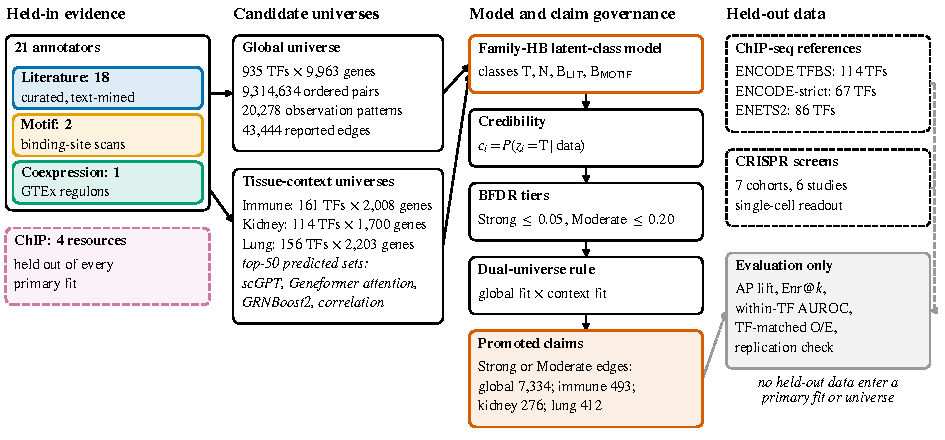
\includegraphics[width=\textwidth]{fig1_design.pdf}
  \caption{\textbf{Study design.} 21 held-in annotators in three evidence families (literature 18, motif 2, coexpression 1) report TF--target edges; the ChIP family (4 resources) is held out of every primary fit. The global universe contains 935 literature-covered TFs $\times$ 9{,}963 genes (9{,}314{,}634 ordered pairs, 20{,}278 distinct observation patterns, 43{,}444 edges with at least one report); the tissue-context universes contain the pairs both foundation models can score (immune 323{,}127, kidney 193{,}686, lung 343{,}512 pairs), in which scGPT and Geneformer attention, GRNBoost2 and correlation define predicted sets (top 50 targets per TF). Family-HB assigns every edge a credibility; BFDR tiers (Strong: BFDR $\leq 0.05$; Moderate: $\leq 0.20$) and, in the tissue universes, the dual-universe rule turn credibilities into graded claims; Strong and Moderate edges are promoted (global 7{,}334; immune 493, kidney 276, lung 412). Held-out ChIP-seq references (ENCODE TFBS, 114 TFs; ENCODE-strict, 67; ENETS2, 86) and 7 CRISPR perturbation cohorts from 6 studies enter no primary fit, universe definition or choice of the primary analysis (dashed: evaluation only); the tuning-optimism analysis uses perturbation labels only to measure what tuning on them would gain, and nothing it selects is used elsewhere.}
  \label{fig:design}
\end{figure}


\section{Related Work}\label{sec:related}

\paragraph{Benchmarking regulatory networks.}
Expression-based network inference methods such as GENIE3 \citep{huynh2010inferring}, GRNBoost2 \citep{moerman2019grnboost2} and SCENIC \citep{aibar2017scenic} are routinely benchmarked against curated or ChIP-derived reference networks, and the resulting method rankings depend strongly on the reference, the candidate set and the metric \citep{pratapa2020benchmarking}.
The same evaluation practice has been carried over to networks read out of single-cell foundation models such as scGPT \citep{cui2024scgpt} and Geneformer \citep{theodoris2023transfer}, typically by ranking TF--target pairs by attention weights.
Restricting the candidate set to pairs with reference coverage inflates precision-type metrics through the denominator alone \citep{kendiukhov2025universe}; we build on this observation by reporting base-rate-normalised quantities throughout and by decomposing any cross-universe difference into base-rate and ranking components.

\paragraph{Integrated regulatory resources.}
Curated TF--target resources are themselves integrations of heterogeneous primary evidence. DoRothEA assigns confidence levels A--E to edges according to the number and type of supporting lines of evidence (literature curation, ChIP-seq, motif scanning, coexpression inference) \citep{garcia2019benchmark}; CollecTRI aggregates literature-derived signed interactions from a dozen resources \citep{mullerdott2023collectri}; OmniPath distributes both together with the per-edge provenance of every primary resource \citep{turei2021omnipath}.
These integration rules are deterministic vote or tier schemes. They do not estimate the reliability of each resource, nor do they account for resources that copy one another, which is the gap a latent-class formulation addresses. We use the DoRothEA levels and CollecTRI membership, recomputed from the held-in evidence only, as established-integration baselines.

\paragraph{Latent-class models without a gold standard.}
Estimating the accuracy of several imperfect classifiers without a reference standard is a classical problem: \citet{dawid1979maximum} introduced maximum-likelihood estimation of observer error rates by the expectation--maximisation (EM) algorithm, \citet{hui1980estimating} the latent-class approach for diagnostic tests, and \citet{raykar2010learning} its Bayesian treatment for crowd-sourced labels. When annotators share sources of error, the conditional-independence assumption fails and accuracy estimates become biased; random-effects and Bayesian latent-class models with conditional dependence between tests were proposed to address this \citep{qu1996random,dendukuri2001bayesian}, and \citet{albert2004cautionary} showed that the choice of dependence structure can matter even when it is not identifiable from the data. Identifiability of latent-class models with many binary indicators is established generically by \citet{allman2009identifiability}. Our family-specific burst classes are a parsimonious latent-class version of conditional dependence, tied to an external grouping of the annotators (evidence modality), and our hierarchical prior pools annotator reliabilities within families.

\paragraph{Combining evidence and controlling false claims.}
Meta-analytic combination rules such as Fisher's and Stouffer's methods, and simple union or majority-vote rules, are standard ways to merge evidence across studies \citep{tseng2012comprehensive}; we include them as baselines. For turning posterior probabilities into claims we use the posterior expected false discovery rate \citep{newton2004detecting}, which, unlike rank budgets, gives tier boundaries a direct error-rate interpretation without reference to validation data.

\paragraph{Perturbation-grounded validation.}
Pooled CRISPR screens with single-cell readout \citep{dixit2016perturb,adamson2016multiplexed,shifrut2018genome,norman2019exploring,papalexi2021characterizing,replogle2022mapping} provide causal, though partly indirect, evidence on TF--target relations that is independent of all curated resources; ChIP-seq occupancy maps from ENCODE \citep{encode2012integrated,gerstein2012architecture} provide binding evidence of a different modality. We use both only for validation.

\section{Methods}\label{sec:methods}

\begin{table}[!t]
  \centering
  \caption{Glossary of terms specific to this paper.}
  \label{tab:glossary}
  \small
  \begin{tabular}{@{}p{0.24\textwidth}p{0.72\textwidth}@{}}
    \toprule
    Term & Meaning \\
    \midrule
    Universe & Set of ordered TF--target pairs under consideration: \emph{global} (literature-covered TFs $\times$ genes) or \emph{tissue-context} (pairs both foundation models can score in a tissue). \\
    Annotator; family & A primary evidence resource; its evidence modality (literature, motif, coexpression; ChIP held out). \\
    Observation pattern & For one edge, which annotators observe it and which of those report it. Edges with equal patterns form a tie block. \\
    Credibility & Posterior probability that an edge is a true regulatory edge, \cref{eq:credibility}. \\
    Burst class & Latent class of non-edges co-reported at an elevated rate within one family. \\
    Predicted set & A method's \nTopK{} highest-scoring targets per TF. \\
    Held-in; held out & Evidence that enters the fit (literature, motif, coexpression annotators); evidence used only for evaluation (ChIP references, perturbation screens). \\
    Curated-conditional observation model & Motif and coexpression annotators observe only edges with held-in literature-curated support; a literature annotator observes the pairs of its TFs and target genes. \\
    MAP; NUTS & Posterior-mode (maximum a posteriori) estimate; No-U-Turn Hamiltonian Monte Carlo sampler. \\
    EM baseline & Two-class Dawid--Skene latent-class model with conditionally independent annotators. \\
    Mode switch & A dropout fit whose selected optimum is not the continuation of the full-data posterior mode. \\
    Design-faithful simulator & Simulation from the fitted model that keeps the real literature masks and rebuilds the curated-conditional masks from the simulated reports. \\
    Evaluable edge & Edge for which a held-out reference can provide a label. \\
    AP lift; $\mathrm{Enr}@k$ & Average precision, or precision of the top $k$ edges, divided by the positive rate of the evaluable edges. \\
    O/E; stratified enrichment & Observed over expected positives under a null with TF effects (TF-matched) or with TF and target-degree effects (stratified). \\
    Composition-adjusted AP lift & AP lift divided by its expectation under random ordering of the edges within each TF. \\
    BFDR & Posterior expected false discovery rate of a set, \cref{eq:bfdr}. \\
    Tier & Strong, Moderate (and, for dual-universe tiers, Conditional, Exploratory): claim grades defined by BFDR thresholds. \\
    Dual-universe tier & Tier combining the levels under the global fit and the tissue-context fit. \\
    Promotion & Reporting an edge as a supported claim (tier Strong or Moderate). \\
    Governance & The rule set mapping credibilities to tiers and promoted claims. \\
    Over-promotion index & Share of selected edges in a TF group divided by the share of held-out positives in that group. \\
    Support floor & Smallest number of promoted evaluable edges giving \nRepPowerPct{}\% power in a study. \\
    L1O, L2O, L3O & Leave-one-, two-, three-study-out refits of the pooled replication model. \\
    \bottomrule
  \end{tabular}
\end{table}

Terms that are specific to this paper are collected in \Cref{tab:glossary}.

\subsection{Notation and observation model}\label{sec:notation}
Let $\mathcal{U}=\{i=(t,g)\}$ be a candidate \emph{universe} of ordered pairs of a transcription factor (TF) $t$ and a target gene $g\neq t$, and let $j=1,\dots,K$ index evidence \emph{annotators}: public primary resources that report TF--target edges (\Cref{sec:data-annotators}).
Each annotator belongs to an evidence-modality \emph{family} $f(j)\in\mathcal{F}$ (literature, motif, coexpression).
An annotator can only be informative about edges it could have reported. We encode this by an observation indicator $o_{ij}\in\{0,1\}$ and, when $o_{ij}=1$, a report $r_{ij}\in\{0,1\}$ ($r_{ij}=1$ if annotator $j$ lists edge $i$).
Under the curated-conditional observation model (\Cref{sec:data-annotators}) a literature annotator observes $(t,g)$ when it covers $t$ and $g$ occurs in it, and a motif or coexpression annotator observes $(t,g)$ when it covers $t$ and the edge has held-in literature-curated support.
The estimators of \Cref{sec:model,sec:ladder} treat the observation indicators as ignorable (missing at random given the design); \Cref{sec:obsmodel} relaxes this assumption.

\subsection{Hierarchical latent-class model with family-specific dependence}\label{sec:model}
Each edge carries a latent class $z_i\in\mathcal{C}=\{\mathrm{T},\mathrm{N}\}\cup\{\mathrm{B}_f: f\in\mathcal{F},\ |f|\ge 2\}$: a true regulatory edge (T), a clean non-edge (N), or a \emph{family-$f$ burst} non-edge ($\mathrm{B}_f$), that is, a non-edge that the annotators of family $f$ co-report at an elevated rate because of a shared artefact such as a copied literature claim or a promiscuous motif.
Burst classes are defined only for families with at least two annotators, because a single annotator cannot distinguish a burst from its own false-positive rate; with the annotators used here these are the literature and motif families.
The generative model, which we call Family-HB, is
\begin{align}
  z_i \mid \mathbf{w} &\sim \mathrm{Categorical}(\mathbf{w}), & \mathbf{w}&\sim\mathrm{Dirichlet}(1,\dots,1), \label{eq:class}\\
  r_{ij}\mid z_i=c,\ o_{ij}=1 &\sim \mathrm{Bernoulli}(\theta_{jc}) \quad\text{independently over } j, \label{eq:emission}
\end{align}
with annotator-specific reporting rates
\begin{equation}
  \theta_{j\mathrm{N}}=\beta_j=\sigma(b_j),\quad
  \theta_{j\mathrm{T}}=\alpha_j=\beta_j+(1-\beta_j)\,\sigma(a_j),\quad
  \theta_{j\mathrm{B}_f}=\begin{cases}\gamma_j=\beta_j+(1-\beta_j)\,\sigma(g_j), & f(j)=f,\\ \beta_j, & f(j)\neq f,\end{cases}
  \label{eq:rates}
\end{equation}
where $\sigma$ is the logistic function.
The parametrisation enforces $\alpha_j>\beta_j$, the usual condition that every annotator reports true edges more often than clean non-edges, and $\gamma_j>\beta_j$.
The true class differs from a burst class in that it raises reporting in \emph{every} family, whereas $\mathrm{B}_f$ raises it only within family $f$. Latent-class models with many conditionally independent binary indicators are generically identifiable up to relabelling~\citep{allman2009identifiability}; how well the data separate T from the literature burst in practice is examined in \Cref{sec:res-fit}.
Annotator parameters are pooled hierarchically within families: for $q\in\{b,a,g\}$,
\begin{equation}
  q_j \sim \mathcal{N}\big(\mu^{q}_{f(j)},\tau_q^2\big),\qquad
  \mu^{q}_{f}\sim\mathcal{N}\big(\mu^{q}_0,\omega_q^2\big),\qquad
  \mu^{q}_0\sim\mathcal{N}(m_q,2^2),\qquad
  \tau_q,\omega_q\sim\mathrm{HalfNormal}(1),
  \label{eq:hier}
\end{equation}
with $m_b=\operatorname{logit}(0.01)$ and $m_a=m_g=0$, implemented in non-centred form.
The quantity reported for every edge is its \emph{credibility}, the posterior probability of the true class,
\begin{equation}
  c_i=P(z_i=\mathrm{T}\mid \mathbf{o}_i,\mathbf{r}_i,\Theta)=
  \frac{w_{\mathrm{T}}\prod_{j:o_{ij}=1}\theta_{j\mathrm{T}}^{r_{ij}}(1-\theta_{j\mathrm{T}})^{1-r_{ij}}}
       {\sum_{c\in\mathcal{C}} w_c\prod_{j:o_{ij}=1}\theta_{jc}^{r_{ij}}(1-\theta_{jc})^{1-r_{ij}}}.
  \label{eq:credibility}
\end{equation}
Under full Bayesian inference we report the posterior mean $\bar c_i=E[c_i\mid\text{data}]$ and a 95\% credible interval.

\paragraph{Pattern collapse.}
The credibility and the likelihood contribution of edge $i$ depend on the data only through its \emph{observation pattern} $(\mathbf{o}_i,\mathbf{r}_i)$. The model is therefore evaluated over the $P$ distinct patterns weighted by their edge counts $n_p$:
\begin{equation}
  \log p(\text{data}\mid\Theta)=\sum_{p=1}^{P} n_p \log\sum_{c\in\mathcal{C}} w_c \prod_{j:o_{pj}=1}\theta_{jc}^{r_{pj}}(1-\theta_{jc})^{1-r_{pj}}.
  \label{eq:collapsed}
\end{equation}
Edges with the same pattern receive identical credibility. All ranking-based procedures below treat such \emph{tie blocks} as indivisible, or average over uniformly random orderings within a block.

\subsection{Estimator ladder and baselines}\label{sec:ladder}
Five latent-class estimators are compared; all are special cases of one implementation:
(1) the \emph{EM baseline}, a two-class Dawid--Skene model~\citep{dawid1979maximum} with independent $\mathcal{N}(m_q,3^2)$ priors on the annotator parameters (named after the expectation--maximisation algorithm of the original proposal; here it is fitted by the same posterior-mode search as the other estimators);
(2) a \emph{dependence-aware} model with one global burst class whose rates satisfy $\beta_j<\gamma_j<\alpha_j$ for every annotator;
(3) a \emph{multifactor} model with two ordered global burst classes ($\beta_j<\gamma_{j1}<\gamma_{j2}<\alpha_j$);
(4) a \emph{family-regularized} model, the two-class model with the hierarchical prior \eqref{eq:hier}; and
(5) \emph{Family-HB}, the full model \eqref{eq:class}--\eqref{eq:hier}.
Burst classes are the latent-class analogue of the conditional-dependence terms used for diagnostic tests without a gold standard~\citep{qu1996random,dendukuri2001bayesian,albert2004cautionary}.

The estimators are compared with three kinds of baseline.
\emph{Combination rules} computed from the observation pattern: union (any report), majority (at least two reports), number and fraction of reporting annotators, number of reporting families, and Fisher's and Stouffer's methods~\citep{fisher1932statistical,stouffer1949american}. For the last two, each annotator contributes the mid-$p$ value of a one-sided binary test whose null reporting probability is the annotator's observed positive rate $\hat\rho_j$ ($p=\hat\rho_j/2$ for a report, $(1+\hat\rho_j)/2$ otherwise); the statistics are $-2\sum_j\log p_{ij}$, referred to $\chi^2_{2|O_i|}$, and $\sum_j\Phi^{-1}(1-p_{ij})/\sqrt{|O_i|}$, where $O_i$ is the set of annotators observing edge $i$. Edges observed by no annotator receive the lowest score.
\emph{Established integration schemes}, recomputed from the held-in evidence only: the DoRothEA confidence level (A to D) and CollecTRI membership with its curation effort.
\emph{Expression-based inference} in the tissue universes (GRNBoost2, GENIE3, correlation; \Cref{sec:data-universes}).

\subsection{Informative-observation extension}\label{sec:obsmodel}
The models above assume that whether an annotator observes an edge carries no information about the edge's class.
Posterior predictive checks reject this assumption (\Cref{sec:res-fit}), so we also examine a selection-model extension in which observation by a literature annotator is itself an emission.
A literature annotator $j$ is \emph{eligible} for edge $(t,g)$ if it covers $t$, and observes the edge if, in addition, $g$ occurs in it. For eligible entries,
\begin{equation}
  o_{ij}\mid z_i=c \sim \mathrm{Bernoulli}(\eta_{jc}),\qquad \eta_{jc}=\begin{cases}\eta_{j\mathrm{T}}, & c=\mathrm{T},\\ \eta_{j\bar{\mathrm{T}}}, & c\neq \mathrm{T},\end{cases}
  \label{eq:obs}
\end{equation}
followed by \eqref{eq:emission} when $o_{ij}=1$; the logits of $\eta_{j\mathrm{T}}$ and $\eta_{j\bar{\mathrm{T}}}$ receive the same hierarchical prior as the other rates, with no ordering imposed.
Observation by motif and coexpression annotators is a deterministic function of the held-in literature records under the curated-conditional model and is conditioned on.
Setting $\eta_{j\mathrm{T}}=\eta_{j\bar{\mathrm{T}}}$ recovers the ignorable model.
We fit this extension to the Dawid--Skene model and to Family-HB.
Because eligibility is a property of the TF whereas occurrence in an annotator is a property of the gene, the observation indicator of one gene is replicated over all eligible TFs; as a sensitivity analysis we also fit a composite likelihood in which the observation term of annotator $j$ is weighted by the reciprocal of the number of TFs eligible for $j$.
This extension was designed after the held-out results had been examined and is reported as a secondary, post hoc analysis; Family-HB with ignorable observation remains the primary model.

\subsection{Inference and convergence diagnostics}\label{sec:inference}
\paragraph{Posterior mode.} We maximise the log posterior density (maximum a posteriori, MAP, estimation), \eqref{eq:collapsed} plus the log prior, in the unconstrained parametrisation (logit rates, log scales, stick-breaking class weights; the Jacobian keeps the mode away from the boundary of the hierarchical scales) with L-BFGS-B and exact gradients from automatic differentiation, from \nMapRestartsHb{} (Family-HB) or \nMapRestartsOther{} (other estimators) starting points drawn uniformly on $[-2,2]$ in every unconstrained coordinate, followed by Newton steps with the exact Hessian. A start has converged when the largest absolute gradient component is below \nGradTol{} at a positive-definite Hessian. Starts are grouped into distinct optima, and the approximate posterior mass of each optimum is obtained by Laplace's method and, for Family-HB, by bridge sampling~\citep{meng1996simulating,gronau2017tutorial} on posterior draws within each mode.

\paragraph{Full posterior.} The posterior of Family-HB is sampled with the No-U-Turn sampler (NUTS) of Hamiltonian Monte Carlo~\citep{hoffman2014nuts} in NumPyro~\citep{phan2019numpyro}: \nNutsChains{} chains of \nNutsWarmup{} warm-up and \nNutsDraws{} retained iterations, target acceptance \nNutsTargetAccept{}, initialised around the dominant mode, with the latent classes marginalised analytically. Convergence is assessed by the rank-normalised split-$\widehat{R}$ and by bulk and tail effective sample sizes~\citep{vehtari2021rank} for every parameter, and by the number of divergent transitions.

\paragraph{Model checking.} Estimators are compared without validation labels by \nCvFolds{}-fold cross-validated held-out log-likelihood with folds formed by TF, and by posterior predictive checks of the number of reporting annotators per edge, of pairwise co-reporting odds ratios within and between families, and of reporting rates.

\paragraph{Simulation from the fitted model.} We simulate data sets from the fitted Family-HB model and refit them with the same multi-start search. The \emph{design-faithful} simulator keeps the real observation masks of the literature annotators, draws latent classes and literature reports from the fitted model, and then rebuilds the curated-conditional masks of the motif and coexpression annotators from the simulated literature records exactly as the evidence builder does for the real data, before drawing their reports. The literature masks themselves are kept, because the fitted reporting rates, applied to the pairs whose target gene a literature annotator does not contain, would generate more reports there than the literature annotators contain in total. Because the fitted model under-predicts literature reports on well-covered edges (\Cref{sec:res-fit}), the simulated data contain only \nSimInfoPctMin{}--\nSimInfoPctMax{}\% of the real number of motif- or coexpression-observed edges, the edges that carry the informative observations (under the curated-conditional model every such edge has a literature report); a variant whose class weights depend on the stratum of literature masks reproduces the real literature report counts and contains \nSimInfoStratPctMin{}--\nSimInfoStratPctMax{}\% of them. Data are generated both from the dominant optimum of the real fit and, for the immune design, from its second optimum. We compare estimated with true parameters, calibrate credibility against the simulated classes, record whether the selected optimum is the true one, and compute the realised false discovery rate of the resulting claim tiers. A simulator that keeps every mask fixed at the real one, which is inconsistent with the simulated literature reports, is reported as a sensitivity analysis in the Supplement. All simulations were defined after the held-out data had been examined (post hoc); they use no held-out data.

\paragraph{Hub-bias simulation (post hoc).} To ask whether concentration of promoted edges on well-studied TFs is a property of the estimators or of the evidence, we simulate universes with known truth (\nSimHubNrep{} replicates per scenario, each of \nSimHubTfs{} TFs and \nSimHubGenes{} target genes).
Each TF has a popularity (study intensity) $u_t$ with $\log u_t\sim\mathcal{N}(0,\nSimHubLogPopSd{}^2)$; popularity deciles are equal-count deciles of $u_t$.
True edges are drawn with a TF degree that is independent of popularity (scenarios \emph{independent} and \emph{copying}) or increases mildly with it (\emph{biological hubs}), and a non-edge is a copied literature claim with a small probability that is constant, except in the \emph{copying} scenario, where it increases with $u_t$.
Simulated literature annotators cover a TF with a probability that increases with $u_t$ and report true and copied edges with popularity-dependent rates, so that their reports are correlated through popularity even given the class; two motif annotators share a TF-level burst of promiscuous-motif false positives, and one coexpression annotator reports independently.
Observation follows the curated-conditional rules of the real data, and rates are calibrated loosely to the real global fit.
Every latent-class estimator is fitted by multi-start MAP, and the combination rules are evaluated at the size of the Family-HB BFDR set.
The \emph{oracle} is the posterior probability of a true edge under the true generative reporting model, with the observation mask treated as ignorable; it shows how much hub concentration the evidence itself supports.
The over-promotion index (\Cref{sec:governance}) is computed relative to the true edges, for the top popularity decile and, to mirror the real-data index, for the top quintile of TFs by number of literature-reported targets.

\paragraph{Complexity.} One evaluation of \eqref{eq:collapsed} and its gradient costs $O(PKS)$ operations with $S=|\mathcal{C}|$ and $P\le\min(N,3^K)$; memory is $O(PK+N)$ including the edge-to-pattern index; pattern compression is one streaming pass of cost $O(NK)$. Measured scaling is reported in \Cref{sec:res-compute}.

\subsection{Held-out evaluation}\label{sec:eval}
\paragraph{Evaluable edges.}
For a ChIP reference, an edge $(t,g)$ of a universe is \emph{evaluable} if the reference assayed $t$ and $g$ belongs to its gene universe; it is positive if the reference contains it.
For a perturbation cohort, an edge is evaluable if the cohort tested the pair and the pair is not excluded as a same-band pair; it is positive if the pair is a positive of the cohort (\Cref{sec:data-heldout}).
The pooled perturbation reference contains every pair evaluable in at least one cohort, positive if positive in at least one.

\paragraph{Metrics.}
Let $b$ be the positive rate among the $N$ evaluable edges, and $\mathrm{P}@k$ the precision of the $k$ highest-ranked evaluable edges.
The \emph{AP lift} is the average precision, computed with whole tie blocks as thresholds, divided by $b$; it equals 1 in expectation for a random ranking.
The \emph{enrichment at $k$} is $\mathrm{Enr}@k=\mathrm{P}@k/b$, where a tie block cut by position $k$ contributes its positive rate to $\mathrm{P}@k$.
Both equal 1 in expectation for a random ranking at any prevalence; unlike raw precision and $F_1$ they do not rise with the positive rate, although their attainable maximum, $1/b$, does.
Because TFs differ greatly in their number of positives, we add two measures that remove TF composition: the \emph{within-TF AUROC}, the mean over TFs of the area under the ROC curve computed within the TF, and the \emph{stratified enrichment}, the ratio of observed positives in a selected set to the number expected from a null in which the probability that $(t,g)$ is positive is $\operatorname{expit}(a_t+d_{\mathrm{bin}(g)})$, with a TF effect and an effect of the decile of the target's in-degree in the reference computed leaving the pair's own TF out. Dropping the target term gives the \emph{TF-matched} expectation.
The \emph{composition-adjusted AP lift} (post hoc, descriptive) divides the AP lift by its exact expectation when the labels are permuted within TFs, so that it equals 1 in expectation for any ranking that orders edges at random within each TF, whatever its ordering between TFs.

\paragraph{Inference.}
Edges of the same TF are not independent, so interval estimates treat the TF as the unit: confidence intervals are percentile intervals of a bootstrap that resamples TFs, and differences between two scores are tested by a paired TF bootstrap.
The exceptions are tests that condition on TF strata: $p$-values for a single score come from permuting scores within TFs, and the stratified trend test and the exact stratified tests of \Cref{sec:governance,sec:replication} condition on the margins of each TF, (TF, target-degree) or (cohort, TF) stratum. These tests treat the edges within a stratum as exchangeable; under dependence between the targets of a TF they are anti-conservative, so we use them as screens and base inference on the TF-cluster bootstrap intervals.
The primary comparison family (post hoc), for each universe and reference, is Family-HB against the EM baseline, Fisher, Stouffer, the vote count, and the DoRothEA and CollecTRI schemes, on AP lift, with Holm adjustment~\citep{holm1979simple}; all other contrasts are descriptive.
This family was fixed after the first held-out results had been seen and is identified as such in the released decision log; no analysis in this paper was pre-registered.

\paragraph{Universe-aware comparison.}
For two universes $A$ and $B$ and a precision-type metric, the ratio of raw values factorises as
\begin{equation}
  \frac{\mathrm{P}@k(A)}{\mathrm{P}@k(B)}=\frac{b_A}{b_B}\times\frac{\mathrm{Enr}@k(A)}{\mathrm{Enr}@k(B)},
  \label{eq:decomp}
\end{equation}
a prevalence ratio times a ranking ratio.
To calibrate a raw difference between a context universe and the global universe we draw random sub-universes of the global universe with the same number of evaluable edges and exactly the same number of positives as the context universe (prevalence-matched null), by sampling edges and, post hoc, by sampling whole TF blocks matched to the context's per-TF sizes, and compare the context value with the null distribution.

\subsection{Robustness to annotator dropout}\label{sec:robustness}
Every estimator and combination rule is refitted after removing one annotator at a time (source dropout), one modality family at a time (family dropout), or all annotators that reached us through one integrator (lineage dropout).
Latent-class models are refitted from the full-data optimum and from random starts, adding starts until at least two random starts reach the best mode found.
Two kinds of stability are measured.
\emph{Method-ranking stability.} Each method $m$ of the tissue universes is scored against a credibility vector $c$ by the posterior-weighted $F_1$ of its predicted set $\mathcal{P}_m$ over all universe edges, $F_1=2\sum_{i\in\mathcal{P}_m}c_i/(|\mathcal{P}_m|+\sum_i c_i)$. For the full-data credibility $c$ and a dropout credibility $c'$, the \emph{rank disagreement} is the fraction of method pairs, among those not tied under either, whose order differs:
\begin{equation}
  D(c,c')=\frac{\big|\{(m,m'):\ \operatorname{sign}\Delta_{mm'}(c)\neq\operatorname{sign}\Delta_{mm'}(c'),\ \Delta_{mm'}(c)\Delta_{mm'}(c')\neq 0\}\big|}{\big|\{(m,m'):\ \Delta_{mm'}(c)\Delta_{mm'}(c')\neq 0\}\big|},
  \label{eq:rankdisagreement}
\end{equation}
with $\Delta_{mm'}(c)=F_1(m;c)-F_1(m';c)$.
\emph{Edge-level stability.} The Spearman correlation between $c$ and $c'$ over edges still observed by some annotator, and the Jaccard index of the sets selected at a fixed size and at a fixed posterior expected false discovery rate.
Summaries are means over dropout configurations with bootstrap intervals over configurations. Paired differences between estimators are means over configurations with intervals from a bootstrap that resamples the dropped sources; these contrasts, the Jaccard index at equal set size and the decomposition by posterior-mode switches (a dropout optimum that is not the continuation of the full-data mode) were defined after the held-out data had been examined (post hoc), and all their intervals are unadjusted.

\subsection{Claim governance}\label{sec:governance}
\emph{Governance} denotes the rule set that turns credibilities into graded claims.
For a set $A$ of edges with posterior mean credibilities $\bar c_i$, the posterior expected false discovery rate is~\citep{newton2004detecting}
\begin{equation}
  \mathrm{BFDR}(A)=\frac{1}{|A|}\sum_{i\in A}(1-\bar c_i).
  \label{eq:bfdr}
\end{equation}
Within a universe, tie blocks are ordered by decreasing credibility; an edge is \emph{Strong} if it lies in the largest prefix of whole blocks with $\mathrm{BFDR}\le \nBfdrStrong{}$, and \emph{Moderate} if it lies in the largest prefix with $\mathrm{BFDR}\le \nBfdrModerate{}$ but is not Strong.
No validation data enter these definitions, and no tie block is ever split.
In a tissue-context universe each edge has two credibilities, one from the fit to the global universe and one from the fit to the context universe itself. The \emph{dual-universe tier} combines the two levels: \emph{Strong} if Strong under both fits; \emph{Moderate} if at least Moderate under both but not Strong under both; \emph{Conditional} if at least Moderate under exactly one; \emph{Exploratory} otherwise.
An edge is \emph{promoted}, that is, reported as a supported claim, if its dual-universe tier is Strong or Moderate; a method's promoted predictions are the promoted edges within its predicted set.
In the global universe, which has a single fit, tiers are the single-fit levels.
Sensitivity of the promoted set is examined over a grid of the two thresholds, over rules shifted by one tier in either direction, for single-fit tiers, for rank budgets in place of error-rate thresholds, and for promotion by simple rules.
The shifted rules order the pairs of single-fit levels of an edge (Strong above Moderate above below Moderate) by the lower and then the higher of the two levels and move every tier boundary by one step: the \emph{lenient} rule also calls an edge Strong if it is Strong under one fit and Moderate under the other, and Moderate if it is Strong under one fit and below Moderate under the other; the \emph{strict} rule calls an edge that is Moderate under both fits Conditional, and an edge that is Moderate under one fit and below Moderate under the other Exploratory.
Whether held-out enrichment declines across the dual tiers is tested by Mantel's extension test for a linear trend~\citep{mantel1963chisquare}, a stratified form of the Cochran--Armitage trend test~\citep{cochran1954some,armitage1955tests}: the association of the held-out label with the ordinal tier score (from Exploratory, lowest, to Strong, highest) over all evaluable edges, stratified by TF or by TF and decile of target degree, conditional on the positive count of each stratum, one-sided for an increasing trend, with Holm adjustment over the tissues and references. Like the exact tests below, it treats the edges within a stratum as exchangeable and is therefore anti-conservative under dependence between the targets of a TF (\Cref{sec:eval}).
Whether a method's predicted set contains fewer promoted edges than expected from its TFs is tested exactly (post hoc): conditional on, for each TF, the number of its universe edges, of its promoted edges and of its predicted edges, the number of promoted predicted edges is a sum of independent hypergeometric counts.
\emph{Concentration} of a promoted set is described by the share of its edges belonging to the most frequent TF or two TFs, the number of TFs, and Pielou's evenness~\citep{pielou1966measurement}. A \emph{deconcentrated} subset of a given size is selected greedily by $\operatorname{logit}(\min(\bar c_i^{\mathrm{glob}},\bar c_i^{\mathrm{ctx}}))-\lambda\, n_{t(i)}$, where $n_t$ counts the edges of TF $t$ already selected; the size and $\lambda$ are chosen without validation data by maximising the harmonic mean of the min--max normalised mean credibility and TF diversity over a grid. This rule, like the threshold grid and the shifted rules, uses no held-out data, but it was fixed when held-out results of other analyses already existed.
The \emph{over-promotion index} of a selected set with respect to a group of TFs is the share of the selected edges that belong to the group divided by the share of held-out positives that do.

\subsection{Cross-cohort replication check}\label{sec:replication}
The replication check asks whether, within a perturbed TF, promoted edges are more often perturbation positives than the TF's other evaluable edges.
The unit of replication is the study.
Let stratum $s$ be a (cohort, TF) pair with $N_s$ evaluable edges, $n_s$ of them promoted and $K_s$ positive, and $X_s$ promoted positives.
The test statistic is $T=\sum_s X_s$, referred to its exact conditional null distribution given all margins (independent hypergeometric $X_s$; the exact Cochran--Mantel--Haenszel test~\citep{mantel1959statistical}); effect sizes are the stratified enrichment $T/\sum_s n_sK_s/N_s$, with a bootstrap interval that resamples TFs within the study, and the Mantel--Haenszel odds ratio.
Because the test treats the edges of a stratum as exchangeable, its $p$-values are anti-conservative when targets of one TF are dependent (\Cref{sec:eval}).
A study \emph{passes} if the stratified enrichment is at least \nRepEndpoint{} with one-sided $p\le\nRepAlpha{}$; pass rates are reported with Wilson intervals~\citep{wilson1927probable}.

\emph{Power and support floor.} Before any replication outcome was computed, the power of this test to detect a \nRepTrueEnrFold{} enrichment at $\alpha=\nRepAlpha{}$ was calculated for every study from its design alone (the $N_s$ and $n_s$ and the overall positive rate), together with the minimum detectable enrichment at \nRepPowerPct{}\% power and a \emph{support floor}, the smallest number of promoted evaluable edges giving \nRepPowerPct{}\% power; the design and the results of this step were stored with a time stamp and a checksum before the outcome step was run.
Studies below the floor are reported as underpowered, not as failures, although they remain in the denominator of the pass rate over all evaluable studies, and studies in which the margins make an enrichment of \nRepEndpoint{} unattainable are identified.

\emph{Pooling.} Per-study effects are combined in a Bayesian random-effects logistic model for the edges of study $u$ and stratum $s$, $\operatorname{logit}P(\text{positive})=a_{u,s}+\theta_u\cdot\mathbb{1}[\text{promoted}]$, with study effects $\theta_u\sim\mathcal{N}(\mu,\sigma^2)$, $\mu\sim\mathcal{N}(0,1)$ and $\sigma\sim\mathrm{HalfNormal}(0.5)$, and stratum intercepts $a_{u,s}\sim\mathcal{N}(m_u,s_u^2)$ with $m_u\sim\mathcal{N}(-4,3^2)$ and $s_u\sim\mathrm{HalfNormal}(2)$ (centred for strata with many positives and non-centred otherwise), fitted by NUTS; the dependence of the conclusions on the priors of $\mu$ and $\sigma$ is reported for \nRepNPriors{} prior specifications, and a variant with TF-specific slopes $\theta_u+\tau\varepsilon_s$, $\tau\sim\mathrm{HalfNormal}(0.5)$, is a post hoc sensitivity analysis.
\emph{Leave-$k$-out.} L1O, L2O and L3O denote refits of the pooled model after removing every subset of one, two or three studies; we report the resulting changes in $\mu$ and in the per-study posterior probabilities of passing.
With few independent studies this analysis is a replication check of limited power, not a validation.

\section{Data}\label{sec:data}

\Cref{fig:design} summarises the design: the evidence that enters the model, the held-out evidence that judges it, and the universes in which both are used.

\subsection{Candidate universes}\label{sec:data-universes}
\paragraph{Tissue-context universes.}
We analyse three tissues of the Tabula Sapiens atlas~\citep{tabula2022}: an immune subset (\nTsCellsImm{} cells), kidney (\nTsCellsKid{} cells, \nTsDonorsKid{} donor) and lung (\nTsCellsLung{} cells).
For each tissue $t$, the \emph{panel} is the set of genes that both foundation models can score: genes present in the scGPT attention matrix (the 5{,}000 most variable genes intersected with the scGPT vocabulary) and in the Geneformer attention matrix, after normalisation to approved HGNC symbols~\citep{seal2023hgnc}.
The \emph{tissue-context universe} $\mathcal{U}_{\mathrm{ctx}}(t)$ consists of all ordered pairs of a panel gene that is a human TF according to \citet{lambert2018human} and a different panel gene (\Cref{tab:universes}).
Its definition uses expression data and model vocabularies only.

\paragraph{Global universe.}
The \emph{global universe} $\mathcal{U}_{\mathrm{glob}}$ contains every TF covered by at least one held-in literature annotator (\nGlobTfs{} TFs) paired with every gene that is a target in at least one held-in literature annotator or belongs to one of the three panels (\nGlobGenes{} genes): \nGlobEdges{} ordered pairs.
It is the universe in which the estimators are compared, because it contains most TFs assayed by the held-out references; every context edge whose TF is covered by a literature annotator is also a global edge with the same observation pattern.
Neither universe is defined with reference to any validation resource.

\paragraph{Method scores.}
For every context edge we record the following scores (\Cref{tab:universes}).
\emph{scGPT attention}: attention weights of the whole-human scGPT checkpoint, averaged over all layers and heads and over the cells in which both genes are input tokens (TF as query, target as key; the transposed direction is kept as a separate score), extracted from the first \nScgptCells{} cells of each processed tissue file. These cells are not a random sample: \nScgptSmartPctLung{}\% of them were profiled by Smart-seq2 in lung (from \nScgptDonorsLung{} donors), and \nScgptSmartPctImm{}\% and \nScgptSmartPctKid{}\% in immune and kidney, against at most \nOtherSmartPctMax{}\% of the randomly sampled cells used for Geneformer and the expression baselines. Smart-seq2 cells typically have more detected genes than droplet-based cells, so the selection may affect the attention results of \Cref{sec:res-governance}, which depend on the number of genes expressed per cell.
\emph{Geneformer attention}: the same quantity for Geneformer V2-104M~\citep{chen2026geneformer}, extracted from a random sample of \nGfCellsImmLung{} (immune, lung) or \nGfCellsKid{} (kidney) cells.
For both models we also compute the attention an edge would receive if every cell spread its attention uniformly over its $L$ input genes (the mean of $1/L$ over co-observing cells; ``uniform null''), and the ratio of observed to uniform attention (``normalised attention'').
\emph{Expression baselines}: GRNBoost2~\citep{moerman2019grnboost2} with the panel TFs as regulators and, for the immune tissue, GENIE3~\citep{huynh2010inferring}, together with absolute Pearson and Spearman correlation, all computed on one random sample of \nExprCells{} cells per tissue; and a uniform random score.
A method's \emph{predicted set} is its \nTopK{} highest-scoring targets per TF; pairs a method cannot score are not predicted, and ties at the \nTopK{}th position are broken by a fixed random key.
Pairs co-observed in few cells dominate the attention rankings (over all pairs of a universe, scored or not, the median number of co-observing cells is \nCoobsScMin{} to \nCoobsScMax{} for scGPT and \nCoobsGfMax{} for Geneformer, and only \nCoobsFiveScPctMin{}--\nCoobsFiveScPctMax{}\% and \nCoobsFiveGfPctMin{}--\nCoobsFiveGfPctMax{}\% of the pairs are co-observed in at least \nFmMinCoobs{} cells), so we additionally report how attention rankings change when they are restricted to pairs co-observed in at least \nFmMinCoobs{} cells, and predicted sets of \nTopKSensLo{} and \nTopKSensHi{} targets per TF (Supplementary Table~\ref{tab:S-fm-sens}).

% provenance: paper/r2/tables/tab_universes.tex generated by src/r2/paper_assets on 2026-10-15 04:06 from data/r2/tables/
%   evidence_summary.csv (modified 2026-10-14 19:28): variant == prespecified_cc & annotator == __ALL__; number of held-in annotators: variant == prespecified_cc & universe == global & annotator != __ALL__
%   fm_universe_summary.csv (modified 2026-10-14 20:43): all tissues
%   grn_baseline_runtime.csv (modified 2026-10-14 19:28): variant == grnboost2 (primary)
\begin{table}[tbp]
\centering
\small
\setlength{\tabcolsep}{3pt}
\caption{Candidate universes. Edges are ordered TF--target pairs; observation patterns are the distinct (observed, reported) vectors over the 21 held-in annotators under the curated-conditional observation model; method coverage is the share of universe edges a method scores.}
\label{tab:universes}
\begin{tabular}{@{}lrrrrrrrrrr@{}}
\toprule
Universe & TFs & Genes & Edges & Patterns & Observed & Reported & \multicolumn{4}{c}{Method coverage (\%)} \\
\cmidrule(lr){8-11}
 & & & & $P$ & (\%) & edges & scGPT & Geneformer & Correlation & GRNBoost2 \\
\midrule
Immune & 161 & 2{,}008 & 323{,}127 & 3{,}388 & 39.6 & 2{,}216 & 50.5 & 20.5 & 82.9 & 42.7 \\
Kidney & 114 & 1{,}700 & 193{,}686 & 2{,}440 & 41.6 & 1{,}439 & 69.7 & 37.2 & 91.2 & 65.6 \\
Lung & 156 & 2{,}203 & 343{,}512 & 3{,}170 & 44.2 & 2{,}178 & 66.7 & 19.8 & 82.4 & 51.6 \\
\midrule
Global & 935 & 9{,}963 & 9{,}314{,}634 & 20{,}278 & 54.6 & 43{,}444 & -- & -- & -- & -- \\
\bottomrule
\end{tabular}
\par\smallskip
\begin{minipage}{\linewidth}\footnotesize
Observed: share of edges observed by at least one held-in annotator. Reported: edges with at least one held-in report. Correlation: Pearson and Spearman correlation (identical coverage). GRNBoost2: share of universe edges returned by the unfiltered primary run. Method scores exist only for the tissue-context universes (--).
\end{minipage}
\end{table}


\subsection{Evidence annotators}\label{sec:data-annotators}
The evidence annotators are primary TF--target resources as integrated by DoRothEA~\citep{garcia2019benchmark} and CollecTRI~\citep{mullerdott2023collectri} and distributed with per-edge provenance by OmniPath~\citep{turei2021omnipath}, together with TRRUST~v2~\citep{han2018trrust}.
Each edge record is assigned to the primary resource that reported it; the same resource reached through both integrators is merged; integrator-level confidence tags are not used as annotators.
Resources are grouped by evidence modality into four families (\Cref{tab:sources}; the full list with versions or access dates, citations and URLs is given in Supplementary Table~\ref{tab:S-sources}, and the family-assignment criterion of every resource in the source table of the code repository):
\emph{literature} (\nNAnnotLit{} annotators: curated and text-mined interactions~\citep{han2018trrust,vazquez2022extri,huang2019geredb,jiang2007tred,essaghir2010tfacts,bovolenta2012htridb,perfetto2016signor,chu2021curation,portales2009pazar,kanehisa2012kegg,carrascopro2018cytreg,orchard2014intact,huntley2015goa,lesurf2016oreganno,yusuf2012tfe,fantom2009transcriptional,kawaji2011fantom,gronostajski2011nfi}),
\emph{motif} (HOCOMOCO~\citep{kulakovskiy2018hocomoco} and JASPAR~\citep{khan2018jaspar} binding-site scans),
\emph{coexpression} (ARACNe~\citep{margolin2006reverse} regulons inferred from GTEx data), and
\emph{ChIP} (ReMap~\citep{cheneby2018remap}, the high-throughput part of PAZAR~\citep{portales2009pazar}, and two ENCODE-derived sets~\citep{gerstein2012architecture}).
The ChIP family is held out of every primary fit because the validation references are ChIP-seq data.
All annotators are public resources; none was constructed from the candidate edges, from model outputs or from the validation data.

\paragraph{Observation model.}
OmniPath distributes DoRothEA confidence levels A to D only, and every such record has literature or ChIP support.
Motif and coexpression records for edges without literature support therefore exist in our data only because a held-out ChIP resource also supports them.
To keep held-out information out of the fit, the \emph{curated-conditional} observation model lets motif and coexpression annotators observe an edge only if the edge has held-in literature-curated support in DoRothEA; a literature annotator observes $(t,g)$ if it covers $t$ and $g$ occurs in it.
A TF is covered by an annotator if the annotator has at least one record for it.
Under this model \nGlobUnobsPct{}\% of the global universe is observed by no annotator and \nGlobReported{} edges carry at least one report; the \nGlobEdgesMio{} million edges collapse to \nGlobPatterns{} distinct observation patterns.
Alternative observation models (motif and coexpression treated as genome-wide; both endpoints required to occur in the annotator), alternative literature panels (without nine very large regulons; without the four annotators that may contain ChIP-derived records; with the two most overlapping text-mining annotators merged; literature only) and a fit that includes the ChIP family are used as sensitivity analyses (\Cref{sec:res-sensitivity}).
So are three alternative family definitions: integrator lineage (CollecTRI, DoRothEA, or both), every annotator its own family (which removes the burst classes and the pooling within families), and data-driven families obtained by average-linkage clustering of the annotators on one minus the phi coefficient of co-reporting among co-observed edges, cut into three clusters, the number of held-in modality families; the agreement of this clustering with the modality families is measured by the adjusted Rand index on the full data, over the cross-validation training folds and over bootstrap resamples of TFs (post hoc).

% provenance: paper/r2/tables/tab_sources.tex generated by src/r2/paper_assets on 2026-10-15 04:06 from data/r2/tables/
%   source_table.csv (modified 2026-10-14 19:27): all rows, grouped by family
\begin{table}[tbp]
\centering
\small
\setlength{\tabcolsep}{4pt}
\caption{Evidence annotators summarised by modality family (full list with versions, access dates and citations in Supplementary Table~\ref{tab:S-sources}).}
\label{tab:sources}
\begin{tabular}{@{}lrrrllp{4.1cm}@{}}
\toprule
Family & $n$ & Edge records & TFs per annotator & Lineage & Role & Annotators \\
\midrule
Literature & 18 & 71{,}074 & 191 (7--841) & C\,7, D\,7, C+D\,4 & held in & \parbox[t]{4.1cm}{\raggedright ExTRI, NTNU.Curated, GEREDB, TRRUST, TRED, TFactS, HTRIdb, SIGNOR, Pavlidis2021, PAZAR, KEGG, CytReg, IntAct, GOA, ORegAnno, TFe, FANTOM4, other literature} \\
Motif & 2 & 17{,}810 & 251 (248--254) & D\,2 & held in & \parbox[t]{4.1cm}{\raggedright HOCOMOCO, JASPAR} \\
Coexpression & 1 & 10{,}931 & 337 & D\,1 & held in & \parbox[t]{4.1cm}{\raggedright ARACNe-GTEx} \\
ChIP & 4 & 278{,}934 & 76.5 (24--296) & D\,2, O\,2 & held out & \parbox[t]{4.1cm}{\raggedright PAZAR-HT, ReMap, ENCODE-proximal, ENCODE-distal} \\
\bottomrule
\end{tabular}
\par\smallskip
\begin{minipage}{\linewidth}\footnotesize
Edge records are summed over the annotators of a family (an edge reported by two annotators counts twice). TFs: median (range) over annotators. Lineage: integrator through which the records reached us (C, CollecTRI; D, DoRothEA; C+D, both; O, OmniPath TF--target interactions); TRRUST records were also read from its own file. Other literature: the DoRothEA curated reviews and NFIRegulomeDB, merged because each has few records. The ChIP family is held out of every primary fit because the validation references are ChIP-seq data.
\end{minipage}
\end{table}


\subsection{Held-out validation data}\label{sec:data-heldout}
\paragraph{ChIP-seq references.}
\emph{ENCODE TFBS} (transcription-factor binding sites): the gene-set library of ENCODE transcription-factor binding profiles distributed by Harmonizome~\citep{rouillard2016harmonizome,encode2012integrated}, restricted to the five main cell lines (union over cell lines and replicates; \nEncTfs{} TFs after restriction to \citet{lambert2018human} TFs). It is permissive: \nEncDensityPct{}\% of all TF--gene pairs are positives.
\emph{ENCODE-strict}: the subset bound in at least \nEncStrictMinLines{} of the five cell lines, for TFs assayed in at least \nEncStrictMinLines{}.
\emph{ENETS2} (named after its distribution file): the filtered proximal regulatory network of \citet{gerstein2012architecture} (\nEnetTfs{} TFs; \nEnetDensityPct{}\% of pairs positive), the specific reference.
A TF is evaluable against a reference only if the reference assayed it, and a gene only if it belongs to the reference's gene universe (\Cref{tab:chip}).

\paragraph{Perturbation cohorts.}
\nCohNCap{} pooled CRISPR screens with single-cell readout from \nCohStudies{} studies provide perturbation evidence (\Cref{tab:cohorts}): \citet{dixit2016perturb} (two time points), \citet{adamson2016multiplexed}, \citet{shifrut2018genome}, \citet{norman2019exploring}, \citet{papalexi2021characterizing} and \citet{replogle2022mapping}, the first five as distributed by scPerturb~\citep{peidli2024scperturb} or with the original cell annotations.
For each perturbed gene with at least \nDeMinCells{} cells we test every gene expressed in at least \nDeMinFracPct{}\% of perturbed or control cells for differential expression against the cohort's non-targeting controls (Welch $t$-test on log-normalised counts; Benjamini--Hochberg adjustment within perturbation~\citep{benjamini1995controlling}).
For the two cohorts with replicate or donor-by-stimulation structure the test is stratified by that structure.
For the genome-scale screen of \citet{replogle2022mapping} we use the published pseudobulk profiles and a normal approximation to the mean $z$-normalised expression.
A pair (perturbed TF, gene) is a \emph{positive} if the adjusted $p<\nDeFdr{}$ and $|\log_2 \text{fold change}|>\nDeMinLfc{}$; pairs in which the gene lies in the same cytogenetic band as the perturbed TF are excluded from both positives and negatives because CRISPR interference and activation can act on neighbouring genes.
Positives include indirect effects of the perturbation.
The two Dixit time points are treated as one study; the Adamson screen perturbed no TF and is therefore not evaluable for TF--target edges.
None of the cohorts enters any fit, universe definition or choice of the primary analysis; the tuning-optimism analysis of \Cref{sec:res-sensitivity} uses them only to measure what tuning on them would gain.

% provenance: paper/r2/tables/tab_chip.tex generated by src/r2/paper_assets on 2026-10-15 04:06 from data/r2/tables/
%   heldout_chip_table.csv (modified 2026-10-14 19:28): all rows
%   heldout_chip_coverage.csv (modified 2026-10-14 19:28): all rows
\begin{table}[tbp]
\centering
\small
\setlength{\tabcolsep}{4pt}
\caption{Held-out ChIP-seq references and the edges they can label (evaluable edges) in each universe.}
\label{tab:chip}
\begin{tabular}{@{}lrrrlrrrr@{}}
\toprule
\multicolumn{4}{c}{Reference} & \multicolumn{5}{c}{Evaluable in universe} \\
\cmidrule(lr){1-4}\cmidrule(lr){5-9}
 & TFs & Edges & Density (\%) & Universe & TFs & Edges & Positives & Density (\%) \\
\midrule
ENCODE TFBS & 114 & 896{,}426 & 35.7 & Global & 107 & 1{,}037{,}801 & 395{,}408 & 38.1 \\
{\footnotesize (permissive)} &  &  &  & Immune & 24 & 46{,}224 & 10{,}985 & 23.8 \\
 &  &  &  & Kidney & 20 & 32{,}860 & 11{,}929 & 36.3 \\
 &  &  &  & Lung & 17 & 36{,}295 & 7{,}156 & 19.7 \\
\addlinespace[2pt]
ENCODE-strict & 67 & 361{,}456 & 24.5 & Global & 65 & 630{,}437 & 165{,}151 & 26.2 \\
{\footnotesize (intermediate)} &  &  &  & Immune & 12 & 23{,}112 & 2{,}548 & 11.0 \\
 &  &  &  & Kidney & 10 & 16{,}430 & 2{,}450 & 14.9 \\
 &  &  &  & Lung & 6 & 12{,}810 & 857 & 6.7 \\
\addlinespace[2pt]
ENETS2 & 86 & 21{,}038 & 1.3 & Global & 82 & 755{,}798 & 10{,}826 & 1.4 \\
{\footnotesize (specific)} &  &  &  & Immune & 21 & 36{,}729 & 511 & 1.4 \\
 &  &  &  & Kidney & 17 & 26{,}503 & 376 & 1.4 \\
 &  &  &  & Lung & 16 & 31{,}616 & 347 & 1.1 \\
\bottomrule
\end{tabular}
\par\smallskip
\begin{minipage}{\linewidth}\footnotesize
Density: positives as a percentage of the reference's TF $\times$ gene grid (reference) or of the evaluable edges (universe). An edge is evaluable if the reference assayed its TF and its target lies in the reference gene universe.

Sources. ENCODE TFBS: \url{https://maayanlab.cloud/static/hdfs/harmonizome/data/encodetf/gene_set_library_crisp.gmt.gz} (Harmonizome dataset updated 2015-04-06 (file Last-Modified 2020-08-03); accessed 2026-10-07); ENETS2: \url{http://encodenets.gersteinlab.org/enets2.Proximal_filtered.txt} (file Last-Modified 2012-03-06 (Nature 2012 supplementary data); accessed 2026-10-07). ENCODE-strict is derived from the ENCODE TFBS file.
\end{minipage}
\end{table}

% provenance: paper/r2/tables/tab_cohorts.tex generated by src/r2/paper_assets on 2026-10-15 04:06 from data/r2/tables/
%   cohort_table.csv (modified 2026-10-14 19:28): all cohorts
%   cohort_universe_overlap.csv (modified 2026-10-14 19:28): universe == global
\begin{table}[tbp]
\centering
\small
\setlength{\tabcolsep}{1.8pt}
\caption{Perturbation cohorts (Dixit d13, Dixit d7, \citet{dixit2016perturb}; Adamson, \citet{adamson2016multiplexed}; Shifrut, \citet{shifrut2018genome}; Norman, \citet{norman2019exploring}; Papalexi, \citet{papalexi2021characterizing}; Replogle, \citet{replogle2022mapping}). Positives: |log$_2$ fold change| and adjusted $p$ thresholds of the primary differential-expression design (Section~\ref{sec:data-heldout}); same-band cis pairs excluded.}
\label{tab:cohorts}
\begin{tabular}{@{}lrrrrrrr@{}}
\toprule
 & Dixit d13 & Dixit d7 & Adamson & Shifrut & Norman & Papalexi & Replogle \\
\midrule
Cell type & K562 & K562 & K562 & \begin{tabular}[t]{@{}r@{}}primary T\\cell\end{tabular} & K562 & \begin{tabular}[t]{@{}r@{}}THP-1\\monocyte\end{tabular} & K562 \\
Modality & CRISPR KO & CRISPR KO & CRISPRi & CRISPR KO & CRISPRa & CRISPR KO & CRISPRi \\
Accession & {\footnotesize GSE90063} & {\footnotesize GSE90063} & {\footnotesize\begin{tabular}[t]{@{}r@{}}GSE90546\\GSM2406681\end{tabular}} & {\footnotesize GSE119450} & {\footnotesize GSE133344} & {\footnotesize GSE153056} & {\footnotesize\begin{tabular}[t]{@{}r@{}}figshare\\20029387\end{tabular}} \\
DE design & pooled $t$ & pooled $t$ & pooled $t$ & stratified $t$ & pooled $t$ & stratified $t$ & pseudobulk $z$ \\
Cells & 15{,}849 & 28{,}034 & 49{,}657 & 25{,}094 & 56{,}971 & 20{,}725 & 310{,}385 \\
Control cells & 3{,}491 & 5{,}381 & 4{,}588 & 3{,}541 & 9{,}702 & 2{,}386 & 10{,}691 \\
Perturbations & 10 & 10 & 82 & 20 & 105 & 25 & 2{,}021 \\
Perturbed TFs & 10 & 10 & 0 & 2 & 44 & 12 & 93 \\
TF positive edges & 9 & 39 & 0 & 1 & 61{,}016 & 8{,}091 & 22{,}278 \\
\addlinespace[3pt]
\multicolumn{8}{@{}l}{\emph{Global universe}} \\
Perturbed TFs & 10 & 10 & 0 & 2 & 39 & 12 & 56 \\
Evaluable pairs & 42{,}490 & 44{,}734 & 0 & 8{,}165 & 176{,}941 & 60{,}396 & 228{,}705 \\
Positive pairs & 3 & 27 & 0 & 0 & 31{,}264 & 4{,}650 & 11{,}187 \\
TFs with a positive & 3 & 3 & 0 & 0 & 39 & 7 & 47 \\
\bottomrule
\end{tabular}
\par\smallskip
\begin{minipage}{\linewidth}\footnotesize
Dixit d13, Dixit d7: essentially no positives at $|\log_2\mathrm{FC}|$ > 0.25 under Cas9 knockout.

TF perturbations whose positives are not robust to the DE design (Jaccard index of the non-cis positives of the pooled and the stratified test < 0.3): Shifrut (MEF2D; 1 of 2 perturbed TFs) and Papalexi (ATF2, IRF7, POU2F2, SPI1, STAT3; 5 of 12 perturbed TFs).

Accession: GEO series (GSE) or sample (GSM), or figshare record; the Adamson labels were re-derived from the GEO cell identities, and the Replogle data are the published pseudobulk profiles. GEM group: one 10x Genomics library (gel bead-in-emulsion batch).

DE design: pooled $t$, Welch $t$-test of the perturbed cells against the non-targeting (or intergenic-guide) controls; stratified $t$, the same test stratified by replicate, or by donor $\times$ stimulation; pseudobulk $z$, approximate $z$-test on the published pseudobulk $z$-scores against controls of the same GEM group (no replicate structure available).
\end{minipage}
\end{table}


\subsection{Software and hardware}\label{sec:data-compute}
All statistical analyses were run with Python~\nPythonVersion{} (NumPy, SciPy, pandas, JAX and NumPyro) on an Apple M2~Pro laptop (\nHwCores{} cores, \nHwRamGiB{}~GiB RAM) without a GPU, starting from previously extracted attention matrices; the hardware and run time of the attention extraction were not recorded and are not part of the reported costs.
Wall-clock time and peak memory per pipeline stage are reported in \Cref{sec:res-compute}.

\section{Results}\label{sec:results}

\subsection{The model can be fitted to convergence, but its posterior is bimodal}\label{sec:res-fit}

\paragraph{Convergence.}
The first question is whether the estimators can be fitted to convergence and whether their posteriors are identified (\Cref{tab:fit}).
Every posterior-mode fit converged: after Newton polishing the largest gradient component of any stored optimum is \nMapGradMax{} and the smallest Hessian eigenvalue is \nMapHessMin{}, so every optimum is a strict local maximum.
The dominant-mode NUTS fits of Family-HB converge for every quantity the likelihood identifies (class weights, annotator rates, credibilities): maximum $\widehat{R}$ \nNutsRhatIdMin{}--\nNutsRhatIdMax{} and minimum bulk effective sample size \nNutsEssIdMin{}--\nNutsEssIdMax{} across the four universes, with at most \nNutsDivMax{} divergent transition.
The only sites with $\widehat{R}$ above \nRhatFlag{} are coordinates of the hierarchical prior in the global fit, family means and non-centred annotator offsets (maximum \nNutsRhatAllGlob{}, bulk ESS \nNutsEssAllGlob{}), which the likelihood constrains only through the annotator rates they combine into; no identified quantity is flagged, and among the per-mode runs used for bridge sampling below only that of the global second mode, whose posterior probability is negligible, is flagged on identified quantities.
Posterior-mode and posterior-mean credibilities agree closely (Spearman correlation at least \nMvnSpMin{}; Jaccard index of the Strong sets \nMvnJacMin{}--\nMvnJacMax{}), and the posterior-mode credibility of every edge lies inside its 95\% credible interval.
Posterior uncertainty nevertheless matters at the margin (post hoc summary): of the edges with posterior mean credibility above 0.5, \nNutsStradGlob{} of \nNutsGtHalfGlob{} in the global universe and \nNutsStradImm{} of \nNutsGtHalfImm{} in the immune universe have a 95\% credible interval that includes 0.5.
% provenance: paper/r2/tables/tab_fit.tex generated by src/r2/paper_assets on 2026-10-15 04:06 from data/r2/tables/
%   fit_convergence.csv (modified 2026-10-14 19:28): fit_id in {family_hb, family_hb_nuts}
%   fit_map_optima.csv (modified 2026-10-14 19:28): fit_id == family_hb & optimum == 1
%   modes_bridge.csv (modified 2026-10-14 20:11): role == primary_estimate & mode == 1; role == raw_noncentred_coordinates (bridge check in the non-centred coordinates)
%   fit_class_weights.csv (modified 2026-10-14 19:28): fit_id == family_hb_nuts & class_name == T
\begin{table}[tbp]
\centering
\small
\setlength{\tabcolsep}{4pt}
\caption{Family-HB fit diagnostics per universe: posterior-mode search, mass of the second optimum, convergence of the dominant-mode NUTS run and the class weight of true edges.}
\label{tab:fit}
\begin{tabular}{@{}lrrrr@{}}
\toprule
 & Global & Immune & Kidney & Lung \\
\midrule
\multicolumn{5}{@{}l}{\emph{Posterior mode (multi-start MAP)}} \\
Observation patterns $P$ & 20{,}278 & 3{,}388 & 2{,}440 & 3{,}170 \\
Restarts & 50 & 50 & 50 & 50 \\
Distinct optima & 2 & 2 & 3 & 4 \\
Restarts at the best optimum & 27 & 29 & 29 & 12 \\
Gap to second optimum (log post.) & 108.3 & 7.5 & 7.9 & 11.6 \\
Second-mode prob., Laplace & $3.9\times 10^{-46}$ & 0.0016 & 0.0073 & $8.9\times 10^{-5}$ \\
Second-mode prob., bridge sampling$^{\dagger}$ & \begin{tabular}[t]{@{}c@{}}$1.8\times 10^{-46}$\\[-1pt]{\scriptsize [$1.1\times 10^{-46}$, $3.1\times 10^{-46}$]}\end{tabular} & \begin{tabular}[t]{@{}c@{}}0.0044\\[-1pt]{\scriptsize [0.0028, 0.0069]}\end{tabular} & \begin{tabular}[t]{@{}c@{}}0.0029\\[-1pt]{\scriptsize [0.0018, 0.0048]}\end{tabular} & \begin{tabular}[t]{@{}c@{}}$6.3\times 10^{-5}$\\[-1pt]{\scriptsize [$3.9\times 10^{-5}$, $1.0\times 10^{-4}$]}\end{tabular} \\
\quad range (draw sets, proposals)$^{\dagger}$ & \begin{tabular}[t]{@{}r@{}}$1.8\times 10^{-46}$--\\$2.1\times 10^{-46}$\end{tabular} & \begin{tabular}[t]{@{}r@{}}0.0044--\\0.0085\end{tabular} & \begin{tabular}[t]{@{}r@{}}0.0022--\\0.0041\end{tabular} & \begin{tabular}[t]{@{}r@{}}$6.3\times 10^{-5}$--\\$7.3\times 10^{-5}$\end{tabular} \\
\addlinespace[3pt]
\multicolumn{5}{@{}l}{\emph{Full posterior (NUTS, dominant mode; 4 chains $\times$ 1{,}000 draws)}} \\
Max.\ $\widehat{R}$, all sites & 1.016 & 1.009 & 1.009 & 1.007 \\
Max.\ $\widehat{R}$, identified sites & 1.004 & 1.003 & 1.004 & 1.006 \\
Min.\ bulk ESS, all sites & 300 & 752 & 848 & 649 \\
Min.\ bulk ESS, identified sites & 1{,}951 & 1{,}676 & 1{,}921 & 1{,}710 \\
Divergent transitions & 0 & 0 & 1 & 1 \\
Class weight $w_{\mathrm{T}}$ [95\% CrI] & \begin{tabular}[t]{@{}c@{}}0.0031\\[-1pt]{\scriptsize [0.0029, 0.0032]}\end{tabular} & \begin{tabular}[t]{@{}c@{}}0.0065\\[-1pt]{\scriptsize [0.0056, 0.0076]}\end{tabular} & \begin{tabular}[t]{@{}c@{}}0.0065\\[-1pt]{\scriptsize [0.0050, 0.0080]}\end{tabular} & \begin{tabular}[t]{@{}c@{}}0.0050\\[-1pt]{\scriptsize [0.0040, 0.0060]}\end{tabular} \\
Expected true edges (observed) & \begin{tabular}[t]{@{}c@{}}15{,}662\\[-1pt]{\scriptsize [15{,}043, 16{,}252]}\end{tabular} & \begin{tabular}[t]{@{}c@{}}836\\[-1pt]{\scriptsize [738, 947]}\end{tabular} & \begin{tabular}[t]{@{}c@{}}522\\[-1pt]{\scriptsize [412, 625]}\end{tabular} & \begin{tabular}[t]{@{}c@{}}751\\[-1pt]{\scriptsize [619, 895]}\end{tabular} \\
Expected true edges (all)$^{\dagger}$ & \begin{tabular}[t]{@{}c@{}}28{,}690\\[-1pt]{\scriptsize [27{,}525, 29{,}797]}\end{tabular} & \begin{tabular}[t]{@{}c@{}}2{,}113\\[-1pt]{\scriptsize [1{,}838, 2{,}417]}\end{tabular} & \begin{tabular}[t]{@{}c@{}}1{,}256\\[-1pt]{\scriptsize [973, 1{,}525]}\end{tabular} & \begin{tabular}[t]{@{}c@{}}1{,}700\\[-1pt]{\scriptsize [1{,}387, 2{,}048]}\end{tabular} \\
\bottomrule
\end{tabular}
\par\smallskip
\begin{minipage}{\linewidth}\footnotesize
Second-mode probability: approximate posterior mass of the second-best optimum relative to all optima (Laplace) or to the two best modes (bridge sampling on per-mode NUTS draws; Monte-Carlo 95\% interval of the bridge estimate, which covers the within-run error only; range: smallest to largest bridge estimate over the draw sets and proposals that were run, i.e. Gaussian and Student-$t$ proposals and, in the tissue universes, a second set of dominant-mode draws). Likelihood-identified sites: class weights, annotator rates and credibilities. Expected true edges: posterior class weight $w_{\mathrm{T}}$ times the number of edges observed by at least one annotator (observed) or of all universe edges (all), with 95\% credible interval.

A further bridge-sampling check in the raw non-centred sampling coordinates$^{\dagger}$ was too imprecise to be informative (relative error of every estimate at least 0.8) and is not shown.

$^{\dagger}$\,Post hoc: defined after the held-out data had been examined.
\end{minipage}
\end{table}


\paragraph{Two modes.}
Family-HB is not unimodal.
Its \nMapRestartsHb{} random starts converge to \nHbNoptGlobImm{} (global, immune), \nHbNoptKid{} (kidney) or \nHbNoptLung{} (lung) distinct optima.
In every universe the credibilities of the runner-up optimum correlate with those of the best optimum (Spearman \nHbSpTwoMin{}--\nHbSpTwoMax{}), but its Strong set shares essentially no edge with the best one (Jaccard at most \nHbJacTwoMax{}); in the global and immune universes the runner-up exchanges the weights of the true class and the literature burst.
The two readings correspond to two explanations of the same data: edges reported by several literature resources are either well-supported regulatory edges or claims that those resources copied from one another.
Only the motif and coexpression annotators, which report true edges more often than burst edges, can distinguish the two, and under the curated-conditional observation model they observe few edges.
The data favour one labelling clearly in the global universe (log-posterior gap \nHbGapGlob{} nats; posterior probability of the second mode by bridge sampling, a post hoc analysis, \nBridgePGlob{}) and moderately in the tissue universes (gaps \nHbGapTisMin{}--\nHbGapTisMax{} nats; second-mode probability \nBridgePImm{} in immune, with Monte Carlo interval [\nBridgePImmLo{}, \nBridgePImmHi{}], \nBridgePKid{} in kidney and \nBridgePLung{} in lung; \Cref{fig:model}b).
The ranges of these estimates over posterior draw sets and bridge proposals are given in \Cref{tab:fit}; a further check in the raw non-centred sampling coordinates (post hoc) was too imprecise to be informative (relative error of every estimate at least \nBridgeNcReMin{}) and is not used.
NUTS chains started at random do not move between the modes ($\widehat{R}$ \nRandRhatMin{}--\nRandRhatMax{}), so the primary posterior is the dominant-mode posterior, and the second mode is assessed separately.
Mixing the second mode into the credibilities at its bridge-sampling weight (post hoc) leaves the tissue tiers essentially unchanged (Strong-set Jaccard with the primary at least \nMgJacBridgeMin{}), but the Strong tier would shrink to \nMgStrongFiveMin{}--\nMgStrongFiveMax{} edges per tissue if the second mode had probability \nMgPFive{}; the promoted set would then remain largely intact (Jaccard at least \nMgPromFiveMin{}, or \nMgPromFiveSameMin{} if the global fit is mixed at the same probability).
Whether the multi-start search selects the right mode was checked in data simulated from the fitted model with the design-faithful simulator of \Cref{sec:inference} (post hoc).
When the data are generated from the real dominant optimum, the dominant optimum of the refit is the true one in a fraction \nSimPdomImm{} [\nSimPdomImmLo{}, \nSimPdomImmHi{}] of \nSimNImm{} immune-design replicates and in \nSimCorrectGlob{} of \nSimNGlob{} global-design replicates, and the Laplace approximation overstates the risk (mean second-mode probability \nSimLapFwd{} against a misselection rate of \nSimMissFwd{}).
When they are generated from the real second optimum, the fraction falls to \nSimPdomRev{} [\nSimPdomRevLo{}, \nSimPdomRevHi{}] of \nSimNRev{} replicates and the Laplace approximation understates the risk (\nSimLapRev{} against \nSimMissRev{}): how often the wrong mode is chosen depends on which reading generated the data.
In both directions wrong selections occur only at small gaps: over both directions and both variants of the simulator (\nSimNFaithful{} replicates) the largest gap at a wrong selection is \nSimWrongGapMax{} nats, smaller than every real gap (\nHbGapTisMin{}--\nHbGapGlob{} nats), and all \nSimNGeReal{} replicates with a gap at least as large as the real immune gap (\nHbGapImm{} nats) selected the true optimum. The fixed-mask sensitivity simulator has \nSimFixedWrongN{} exception: a replicate in which no restart reached the true mode selected the wrong one at a gap of \nSimFixedWrongGapMax{} nats.
Most of these replicates come from the global design or from the variant with stratum-dependent class weights, however: in the primary simulator, \nSimNGeRealImmCc{} of the \nSimNImm{} immune-design replicates generated from the dominant optimum and none of the \nSimNRev{} generated from the second optimum reach the real immune gap, which lies at the \nSimGapPctImm{} percentile of the simulated immune-design gaps (\nSimGapPctImmStrat{} with stratum-dependent class weights).
A gap of that size is therefore typical of the dominant reading but only weak evidence against the other one: the Wilson upper bound for reaching it from the second optimum (\nSimRevGeHi{}) lies inside the interval for reaching it from the dominant optimum (\nSimFwdGe{} [\nSimFwdGeLo{}, \nSimFwdGeHi{}]).
When the wrong mode is selected, the Strong and Moderate tiers are almost entirely false (realised false discovery rate of the Strong tier \nSimFdrWrong{} in both directions) while their nominal BFDR gives no warning (Supplementary Table~\ref{tab:S-modes-sim}).
\emph{Implication:} the claim tiers are conditional on the dominant mode; we report the bridge-sampling evidence for that mode and the sensitivity of the tiers to its mass, but neither protects against selecting the wrong mode, and identifiability of the literature burst is the main statistical weakness of the model.
% generated by src/r2/paper_assets (make_paper_assets.py figures); do not edit by hand
% provenance: fig2_model generated by src/r2/paper_assets on 2026-10-15 04:07 from data/r2/tables/
%   fit_source_parameters.csv (modified 2026-10-14 19:28): universe = global, fit_id = family_hb_nuts, parameter in {alpha, beta}
%   modes_bridge.csv (modified 2026-10-14 20:11): role = primary_estimate, mode = 1 (second mode); coords = centred, proposal = mvn
%   modes_simulation_replicates.csv (modified 2026-10-14 20:12): simulator = faithful_cc (design-faithful); dominant_is_truth, dominant_strong_realised_fdr
%   modes_simulation.csv (modified 2026-10-14 20:12): stratum in {dominant_is_truth, dominant_not_truth, all}; quantity in {dominant_strong_realised_fdr_mean, dominant_strong_claimed_bfdr_mean, p_dominant_is_truth}; simulator = faithful_cc (primary); faithful_cc_strat and fixed_masks (sensitivity, caption only)
%   modes_faithful_design.csv (modified 2026-10-14 20:12): quantity = n_edges_cc_observed, sim_label in {immune_cc, global_cc}: ratio_sim_mean_to_real (share of the real motif/coexpression-observed edges)
%   fit_modes.csv (modified 2026-10-14 19:29): w_T and w_2 (= class B_LIT; class order T, N, B_LIT, B_MOTIF as in fit_class_weights) of optimum 0 and 1
\begin{figure}[tbp]
  \centering
  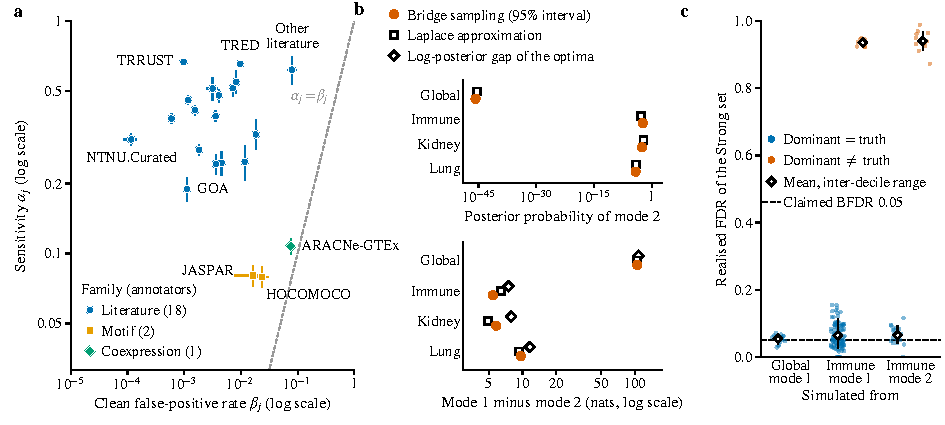
\includegraphics[width=\textwidth]{fig2_model.pdf}
  \caption{\textbf{Family-HB parameters and posterior modes.} (a) Annotator sensitivity $\alpha_j$ against clean false-positive rate $\beta_j$ (posterior means with 95\% credible intervals, global universe, NUTS) for the 21 held-in annotators (18 literature); the dashed diagonal is $\alpha_j=\beta_j$, which the parametrisation excludes. Sensitivities range from 0.08 to 0.67 and false-positive rates from 0.00012 to 0.079. (b) Mode 1 is the dominant posterior mode of each universe fit and mode 2 the second (in the global and immune fits, whose class weights are stored for both modes, mode 2 approximately exchanges the weights of the true class and the literature-burst class). Top: posterior probability of mode 2 by bridge sampling (filled; Monte Carlo 95\% interval) and by Laplace's method (open squares). Bottom: mode 1 minus mode 2 in log posterior mass (bridge sampling, filled; Laplace's method, open squares) and the log-posterior gap of the two optima (diamonds). Values and ranges in Table~\ref{tab:fit}. (c) Mode-selection simulation from the fitted model with the design-faithful simulator (data simulated at the parameters of the indicated mode with the real literature observation masks and the motif/coexpression masks rebuilt from the simulated literature reports, as in the evidence builder; the simulated data contain 59\% (immune) and 62\% (global) of the real number of motif- or coexpression-observed edges; refitted by multi-start MAP): realised false discovery rate of the Strong set for replicates whose dominant mode is or is not the truth mode (points: replicates; diamonds: mean with inter-decile range over replicates; dashed line: claimed BFDR 0.05); global universe, truth = mode 1: dominant mode is the truth mode in all 20 replicates, mean realised FDR 0.05; immune universe, truth = mode 1: dominant mode is the truth mode in 93 of 100 replicates, mean realised FDR 0.06 when it is and 0.94 when it is not; immune universe, truth = mode 2: dominant mode is the truth mode in 18 of 30 replicates, mean realised FDR 0.06 when it is and 0.94 when it is not. Sensitivity, probability that the dominant mode is the truth mode with every observation mask fixed at the real one: global universe 0.70, immune universe 0.68, immune universe (truth = mode 2) 0.77; with class weights that depend on the literature-mask stratum: global universe 1.00, immune universe 1.00, immune universe (truth = mode 2) 0.97 (Supplementary Table~\ref{tab:S-modes-sim}). The bridge-sampling estimates in (b) and panel (c) are post hoc (defined after the held-out data had been examined; no held-out data are used).}
  \label{fig:model}
\end{figure}


\paragraph{Which annotators carry information.}
Under the global fit the most diagnostic annotators, measured by the likelihood ratio of a report under the true class against the mixture of all non-true classes (post hoc summaries of the global NUTS fit), are SIGNOR (\nLrSignor{} [\nLrSignorLo{}, \nLrSignorHi{}]), TRRUST (\nLrTrrust{} [\nLrTrrustLo{}, \nLrTrrustHi{}]) and HTRIdb (\nLrHtridb{} [\nLrHtridbLo{}, \nLrHtridbHi{}]); motif and coexpression reports are only weakly diagnostic (Supplementary Table~\ref{tab:S-annotator-params}).
NTNU.Curated, which would look most diagnostic if only clean negatives were considered, ranks \nLrNtnuRank{} (\nLrNtnu{} [\nLrNtnuLo{}, \nLrNtnuHi{}]) because it reports burst edges more often than true edges ($\alpha/\gamma=\nAgNtnu{}$ [\nAgNtnuLo{}, \nAgNtnuHi{}]): about \nNtnuInExtriPct{}\% of its edges are also reported by the text-mining resource ExTRI.
The EM baseline, which assumes conditional independence, counts such co-reports as independent confirmation, and its Strong set is \nStrongRatioGlob{} times larger than that of Family-HB in the global universe (\nStrongEmGlob{} versus \nStrongHbGlob{} edges, posterior-mode credibilities).
In data simulated from the fitted Family-HB model (design-faithful simulator; \nRecNImm{} immune-design and \nRecNGlob{} global-design replicates) the EM Strong set has a realised false discovery rate of \nRecFdrEmMin{}--\nRecFdrEmMax{}, against \nRecFdrHbTruth{} for Family-HB when its fit selects the true mode; the immune value over all replicates, \nRecFdrHbImm{}, includes the \nRecNCompImm{} replicates whose fit selected the competing mode (Supplementary Table~\ref{tab:S-recovery}).
Because these data are generated with the dependence structure that Family-HB estimates, the comparison favours Family-HB by construction; it shows what ignoring the dependence costs if the dependence is as Family-HB estimates, not that the real data have this structure.

\paragraph{Label-free model checking.}
Without using any validation label, \nCvFolds{}-fold cross-validation with folds formed by TF prefers the burst models: the held-out log-likelihood per observed edge of the EM baseline is lower than that of Family-HB by \nCvEmGlob{} ($\pm$\nCvEmGlobSe{}) nats in the global universe and \nCvEmImm{} ($\pm$\nCvEmImmSe{}) in the immune universe, in all \nCvFoldsHbBetter{} folds of the two universes.
Posterior predictive checks reveal a misfit that all five estimators share: the probability that an edge is reported by at least one literature resource rises much faster with the number of literature resources that cover it than any model predicts (Supplementary Fig.~\ref{fig:S-ppc}; observed \nPpcObsOne{} versus predicted \nPpcRepOne{} for edges covered by one resource; observed \nPpcObsEight{} versus predicted \nPpcRepEight{} for edges covered by eight or more).
Well-studied gene pairs are covered by many resources and reported by many of them, a dependence on study intensity that none of the latent-class models represents.
This misfit is the first sign of the failure examined in \Cref{sec:res-heldout}.


\subsection{Family-HB is not more robust to annotator dropout than simpler estimators}\label{sec:res-robustness}

Removing one annotator at a time barely changes how any estimator ranks the \nRobNMethodsImm{} (immune) or \nRobNMethodsKidLung{} (kidney, lung) inference methods of the tissue universes (\Cref{tab:robustness}, \Cref{fig:robustness}).
Pooled over tissues and the \nRobNconf{} source-dropout configurations, the mean rank disagreement $D$ is \nRobDUnion{} for union, \nRobDVote{} for vote fraction, \nRobDEm{} for the EM baseline, \nRobDMaj{} for majority, \nRobDHb{} for Family-HB, \nRobDDep{} for the dependence-aware model, \nRobDSto{} for Stouffer, \nRobDFis{} for Fisher and \nRobDMf{} for the multifactor model.
Paired against EM over the same configurations (source-clustered, unadjusted 95\% intervals), every model with a burst class is less stable than EM: Family-HB slightly, by \nRobCtHbEm{} [\nRobCtHbEmLo{}, \nRobCtHbEmHi{}] (the interval only just excludes 0; \Cref{tab:robustness}), and, in post hoc contrasts with EM, the dependence-aware model by \nRobCtDepEm{} [\nRobCtDepEmLo{}, \nRobCtDepEmHi{}] and the multifactor model by \nRobCtMfEm{} [\nRobCtMfEmLo{}, \nRobCtMfEmHi{}].
Fisher, Stouffer and majority are also less stable than EM (post hoc; differences \nRobCtRuleEmMin{}--\nRobCtRuleEmMax{}), whereas union and vote fraction are not distinguishable from it.
% provenance: paper/r2/tables/tab_robustness.tex generated by src/r2/paper_assets on 2026-10-15 04:06 from data/r2/tables/
%   rob_method_ranking.csv (modified 2026-10-14 19:32): tissue == all_tissues & metric == f1 & subset in {all, no_fhb_mode_switch}; lineage: subset == excl_uninformative (configurations in which Family-HB is identified, the same for every estimator)
%   rob_estimator_contrasts.csv (modified 2026-10-14 19:32): scope == all_tissues & metric == D_f1 & reference == family_hb & protocol == source & subset in {all, no_fhb_mode_switch}
%   rob_edge_stability.csv (modified 2026-10-14 19:32): universe == global & protocol == source & subset == all
%   robustness.py.csv: NEAR_BEST (log-posterior distance counted as the same mode)
\begin{table}[tbp]
\centering
\small
\caption{Robustness to annotator dropout. (a) Rank disagreement $D$ of the tissue-method ranking (posterior-weighted $F_1$), three tissue universes pooled, with and without the configurations in which Family-HB switches posterior mode. (b) Edge-level stability in the global universe under single-source dropout (21 configurations): full-data sets against dropout sets.}
\label{tab:robustness}
{
\footnotesize
\setlength{\tabcolsep}{4pt}
\par\noindent\emph{(a) Method ranking, tissue universes}\par\smallskip
\begin{tabular}{@{}lcccccc@{}}
\toprule
 & \multicolumn{2}{c}{Source dropout (63)} & \multicolumn{2}{c}{Without mode switches (61)$^{\dagger}$} & Family (9) & Lineage (6)$^{\dagger}$ \\
\cmidrule(lr){2-3}\cmidrule(lr){4-5}
Estimator & $D$ & $\Delta D$ & $D$ & $\Delta D$ & $D$ & $D$ \\
\midrule
\multicolumn{7}{@{}l}{\emph{Latent-class estimators}} \\
EM baseline & \begin{tabular}[t]{@{}c@{}}0.008\\[-1pt]{\scriptsize [0.003, 0.015]}\end{tabular} & \begin{tabular}[t]{@{}c@{}}$-$0.008\\[-1pt]{\scriptsize [$-$0.017, $-$0.0001]}\end{tabular} & \begin{tabular}[t]{@{}c@{}}0.008\\[-1pt]{\scriptsize [0.003, 0.015]}\end{tabular} & \begin{tabular}[t]{@{}c@{}}$-$0.004\\[-1pt]{\scriptsize [$-$0.009, 0.001]}\end{tabular} & \begin{tabular}[t]{@{}c@{}}0.220\\[-1pt]{\scriptsize [0.000, 0.660]}\end{tabular} & \begin{tabular}[t]{@{}c@{}}0.065\\[-1pt]{\scriptsize [0.032, 0.098]}\end{tabular} \\
Dependence-aware & \begin{tabular}[t]{@{}c@{}}0.017\\[-1pt]{\scriptsize [0.009, 0.025]}\end{tabular} & \begin{tabular}[t]{@{}c@{}}0.000\\[-1pt]{\scriptsize [$-$0.009, 0.008]}\end{tabular} & \begin{tabular}[t]{@{}c@{}}0.016\\[-1pt]{\scriptsize [0.009, 0.025]}\end{tabular} & \begin{tabular}[t]{@{}c@{}}0.004\\[-1pt]{\scriptsize [$-$0.002, 0.010]}\end{tabular} & \begin{tabular}[t]{@{}c@{}}0.220\\[-1pt]{\scriptsize [0.000, 0.647]}\end{tabular} & \begin{tabular}[t]{@{}c@{}}0.153$^{b}$\\[-1pt]{\scriptsize [0.100, 0.206]}\end{tabular} \\
Multifactor & \begin{tabular}[t]{@{}c@{}}0.058\\[-1pt]{\scriptsize [0.039, 0.080]}\end{tabular} & \begin{tabular}[t]{@{}c@{}}0.041\\[-1pt]{\scriptsize [0.023, 0.059]}\end{tabular} & \begin{tabular}[t]{@{}c@{}}0.058\\[-1pt]{\scriptsize [0.038, 0.079]}\end{tabular} & \begin{tabular}[t]{@{}c@{}}0.046\\[-1pt]{\scriptsize [0.029, 0.065]}\end{tabular} & \begin{tabular}[t]{@{}c@{}}0.309\\[-1pt]{\scriptsize [0.061, 0.712]}\end{tabular} & \begin{tabular}[t]{@{}c@{}}0.176$^{b}$\\[-1pt]{\scriptsize [0.166, 0.186]}\end{tabular} \\
Family-regularized & \begin{tabular}[t]{@{}c@{}}0.009\\[-1pt]{\scriptsize [0.003, 0.015]}\end{tabular} & \begin{tabular}[t]{@{}c@{}}$-$0.008\\[-1pt]{\scriptsize [$-$0.017, 0.000]}\end{tabular} & \begin{tabular}[t]{@{}c@{}}0.009\\[-1pt]{\scriptsize [0.004, 0.015]}\end{tabular} & \begin{tabular}[t]{@{}c@{}}$-$0.004\\[-1pt]{\scriptsize [$-$0.009, 0.001]}\end{tabular} & \begin{tabular}[t]{@{}c@{}}0.218\\[-1pt]{\scriptsize [0.000, 0.654]}\end{tabular} & \begin{tabular}[t]{@{}c@{}}0.065\\[-1pt]{\scriptsize [0.032, 0.098]}\end{tabular} \\
Family-HB & \begin{tabular}[t]{@{}c@{}}0.017\\[-1pt]{\scriptsize [0.009, 0.025]}\end{tabular} & -- & \begin{tabular}[t]{@{}c@{}}0.012\\[-1pt]{\scriptsize [0.007, 0.017]}\end{tabular} & -- & \begin{tabular}[t]{@{}c@{}}0.227\\[-1pt]{\scriptsize [0.000, 0.449]}\end{tabular} & \begin{tabular}[t]{@{}c@{}}0.120$^{b}$\\[-1pt]{\scriptsize [0.090, 0.151]}\end{tabular} \\
\addlinespace[3pt]
\multicolumn{7}{@{}l}{\emph{Combination rules}} \\
Union & \begin{tabular}[t]{@{}c@{}}0.005\\[-1pt]{\scriptsize [0.002, 0.009]}\end{tabular} & \begin{tabular}[t]{@{}c@{}}$-$0.012\\[-1pt]{\scriptsize [$-$0.021, $-$0.003]}\end{tabular} & \begin{tabular}[t]{@{}c@{}}0.005\\[-1pt]{\scriptsize [0.002, 0.008]}\end{tabular} & \begin{tabular}[t]{@{}c@{}}$-$0.007\\[-1pt]{\scriptsize [$-$0.012, $-$0.003]}\end{tabular} & \begin{tabular}[t]{@{}c@{}}0.037\\[-1pt]{\scriptsize [0.000, 0.111]}\end{tabular} & \begin{tabular}[t]{@{}c@{}}0.035\\[-1pt]{\scriptsize [0.023, 0.048]}\end{tabular} \\
Majority ($\geq$2) & \begin{tabular}[t]{@{}c@{}}0.014\\[-1pt]{\scriptsize [0.008, 0.019]}\end{tabular} & \begin{tabular}[t]{@{}c@{}}$-$0.003\\[-1pt]{\scriptsize [$-$0.012, 0.004]}\end{tabular} & \begin{tabular}[t]{@{}c@{}}0.013\\[-1pt]{\scriptsize [0.008, 0.019]}\end{tabular} & \begin{tabular}[t]{@{}c@{}}0.001\\[-1pt]{\scriptsize [$-$0.004, 0.006]}\end{tabular} & \begin{tabular}[t]{@{}c@{}}0.073\\[-1pt]{\scriptsize [0.006, 0.195]}\end{tabular} & \begin{tabular}[t]{@{}c@{}}0.066\\[-1pt]{\scriptsize [0.047, 0.085]}\end{tabular} \\
Vote fraction & \begin{tabular}[t]{@{}c@{}}0.007\\[-1pt]{\scriptsize [0.003, 0.012]}\end{tabular} & \begin{tabular}[t]{@{}c@{}}$-$0.009\\[-1pt]{\scriptsize [$-$0.018, $-$0.002]}\end{tabular} & \begin{tabular}[t]{@{}c@{}}0.006\\[-1pt]{\scriptsize [0.003, 0.010]}\end{tabular} & \begin{tabular}[t]{@{}c@{}}$-$0.006\\[-1pt]{\scriptsize [$-$0.011, $-$0.002]}\end{tabular} & \begin{tabular}[t]{@{}c@{}}0.059\\[-1pt]{\scriptsize [0.000, 0.160]}\end{tabular} & \begin{tabular}[t]{@{}c@{}}0.051\\[-1pt]{\scriptsize [0.036, 0.065]}\end{tabular} \\
Fisher & \begin{tabular}[t]{@{}c@{}}0.022\\[-1pt]{\scriptsize [0.014, 0.032]}\end{tabular} & \begin{tabular}[t]{@{}c@{}}0.005\\[-1pt]{\scriptsize [$-$0.006, 0.016]}\end{tabular} & \begin{tabular}[t]{@{}c@{}}0.022\\[-1pt]{\scriptsize [0.013, 0.032]}\end{tabular} & \begin{tabular}[t]{@{}c@{}}0.010\\[-1pt]{\scriptsize [0.002, 0.019]}\end{tabular} & \begin{tabular}[t]{@{}c@{}}0.100\\[-1pt]{\scriptsize [0.019, 0.250]}\end{tabular} & \begin{tabular}[t]{@{}c@{}}0.078\\[-1pt]{\scriptsize [0.038, 0.117]}\end{tabular} \\
Stouffer & \begin{tabular}[t]{@{}c@{}}0.019\\[-1pt]{\scriptsize [0.011, 0.029]}\end{tabular} & \begin{tabular}[t]{@{}c@{}}0.003\\[-1pt]{\scriptsize [$-$0.006, 0.012]}\end{tabular} & \begin{tabular}[t]{@{}c@{}}0.019\\[-1pt]{\scriptsize [0.011, 0.030]}\end{tabular} & \begin{tabular}[t]{@{}c@{}}0.007\\[-1pt]{\scriptsize [0.000, 0.015]}\end{tabular} & \begin{tabular}[t]{@{}c@{}}0.081\\[-1pt]{\scriptsize [0.006, 0.225]}\end{tabular} & \begin{tabular}[t]{@{}c@{}}0.063\\[-1pt]{\scriptsize [0.028, 0.098]}\end{tabular} \\
\bottomrule
\end{tabular}
}
\par\medskip
{
\footnotesize
\setlength{\tabcolsep}{5pt}
\par\noindent\emph{(b) Edges, global universe}\par\smallskip
\begin{tabular}{@{}lrccc@{}}
\toprule
 & & \multicolumn{2}{c}{Jaccard index [95\% CI]} &  \\
\cmidrule(lr){3-4}
Estimator & $|S|$ & BFDR\,$\le$\,0.05 set & Size-matched$^{\dagger}$ & Spearman \\
\midrule
\multicolumn{5}{@{}l}{\emph{Latent-class estimators}} \\
EM baseline & 18{,}873 & 0.92 [0.85, 0.98] & 0.88 [0.80, 0.95] & 0.980 \\
Dependence-aware & 3{,}842 & 0.84 [0.74, 0.92] & 0.88 [0.81, 0.93] & 0.972 \\
Multifactor & 223 & 0.80 [0.69, 0.90] & 0.80 [0.71, 0.87] & 0.965 \\
Family-regularized & 18{,}873 & 0.92 [0.85, 0.98] & 0.88 [0.80, 0.95] & 0.980 \\
Family-HB & 4{,}064 & 0.85 [0.76, 0.92] & 0.87 [0.81, 0.92] & 0.979 \\
\addlinespace[3pt]
\multicolumn{5}{@{}l}{\emph{Combination rules}} \\
Union & 43{,}444 & 0.97 [0.94, 0.99] & 0.95 [0.91, 0.98] & 0.986 \\
Majority ($\geq$2) & 17{,}086 & 0.95 [0.90, 0.98] & 0.91 [0.85, 0.96] & 0.971 \\
Vote fraction & 4{,}992 & 0.92 [0.86, 0.96] & 0.90 [0.82, 0.96] & 0.986 \\
Fisher & 26{,}796 & 0.94 [0.90, 0.97] & 0.86 [0.80, 0.92] & 0.982 \\
Stouffer & 21{,}243 & 0.93 [0.88, 0.97] & 0.86 [0.80, 0.92] & 0.986 \\
\bottomrule
\end{tabular}
}
\par\smallskip
\begin{minipage}{\linewidth}\footnotesize
Lineage dropout$^{\dagger}$: the 6 configurations in which Family-HB is identified, for every estimator (the other 3 of 9 leave one modality family); Family-HB switches posterior mode in 4 of them. $^{b}$\,Includes dropout fits whose optimum was found only by the extended start search or the independent-seed check (post hoc).

$\Delta D$: paired difference to Family-HB (negative: more stable). Intervals: unadjusted 95\% bootstrap intervals over configurations clustered by the dropped source, family or lineage (one cluster across the three tissues$^{\dagger}$); family and lineage dropout (three families or lineages per tissue): descriptive. Mode switches$^{\dagger}$: in 2 of 63 source configurations (lung, SIGNOR and TRRUST dropped) the selected Family-HB dropout optimum is not the continuation of the full-data mode (warm-started fit more than $1.0\times 10^{-3}$ log-posterior units below it); the right-hand source columns drop them for every estimator, which conditions on the Family-HB fit and decomposes, but does not replace, the prespecified columns.

(b) $|S|$: size of the full-data posterior-mode BFDR\,$\le$\,0.05 set (for a 0/1 rule its positives, several times the Family-HB set, which favours the rules' Jaccard index); size-matched: top $n$ edges, $n$ the size of the Family-HB set; Spearman: scores of observed edges. One configuration per source, so the intervals are source-clustered; no Family-HB mode switch.

$^{\dagger}$\,Post hoc: defined after the held-out data had been examined.
\end{minipage}
\end{table}

% generated by src/r2/paper_assets (make_paper_assets.py figures); do not edit by hand
% provenance: fig3_robustness generated by src/r2/paper_assets on 2026-10-15 04:07 from data/r2/tables/
%   rob_method_ranking.csv (modified 2026-10-14 19:32): tissue = all_tissues, metric = f1, subset in {all, no_fhb_mode_switch (post hoc)}; lineage: subset = excl_uninformative (post hoc; the configurations in which Family-HB is identified, the same for every estimator); source-clustered intervals mean_D_cluster_lo/hi
%   rob_edge_stability.csv (modified 2026-10-14 19:32): protocol = source, subset = all; jaccard_bfdr_mean and jaccard_top_sizematched_mean (post hoc) with bootstrap intervals over configurations
%   rob_estimator_contrasts.csv (modified 2026-10-14 19:32): reference = family_hb, subset = all, scope = all_tissues (D_f1) or universe (jaccard_bfdr)
%   (constants): bfdr_strong from r2.common.PRESPECIFIED
\begin{figure}[tbp]
  \centering
  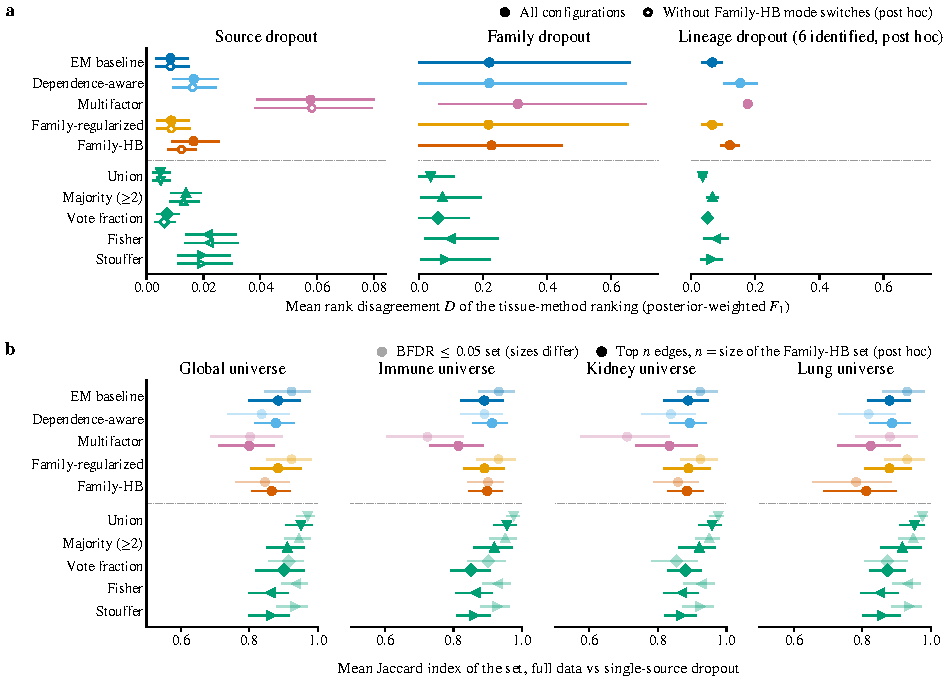
\includegraphics[width=\textwidth]{fig3_robustness.pdf}
  \caption{\textbf{Robustness to annotator dropout.} (a) Mean rank disagreement $D$ \eqref{eq:rankdisagreement} between the method ranking under the full-data credibility and under dropout of one source, one modality family or one integrator lineage, pooled over the three tissue universes (63 source, 9 family and 6 lineage configurations), with 95\% bootstrap intervals clustered by the dropped source, family or lineage (post hoc); family and lineage intervals are descriptive (at most three configurations per universe). Source dropout: Family-HB 0.017 [0.009, 0.025], EM 0.008 [0.003, 0.015], union 0.005 [0.002, 0.009]; open markers (post hoc): the 61 configurations left after removing the 2 in which Family-HB switches posterior mode (lung, SIGNOR and TRRUST dropped), Family-HB 0.012 [0.007, 0.017], EM 0.008 [0.003, 0.015]. Lineage dropout (post hoc): the 6 configurations in which Family-HB is identified, for every estimator (dropping the DoRothEA lineage leaves one modality family, so Family-HB is not identified in 3 of the 9 lineage configurations; post hoc identification rule): Family-HB 0.120 [0.090, 0.151], EM 0.065 [0.032, 0.098]; Family-HB switches posterior mode in 4 of them. (b) Mean Jaccard index between the full-data and the single-source dropout sets (faded markers: BFDR $\leq 0.05$ set; filled markers (post hoc): top $n$ edges, $n$ the size of the Family-HB set), with 95\% bootstrap intervals over the dropout configurations (one per source). For a 0/1 rule the BFDR set is its set of positives, several times larger than the Family-HB set (global universe: Family-HB 4{,}064, EM 18{,}873, union 43{,}444 edges), which inflates its Jaccard index. Global universe, BFDR set: Family-HB 0.85 [0.76, 0.92], EM 0.92 [0.85, 0.98], union 0.97 [0.94, 0.99]; size-matched: Family-HB 0.87 [0.81, 0.92], EM 0.88 [0.80, 0.95], union 0.95 [0.91, 0.98]. The Family-HB values of the lung universe include the source configurations in which Family-HB switches posterior mode (lung, SIGNOR and TRRUST dropped; size-matched Family-HB lung 0.81 [0.69, 0.90]).}
  \label{fig:robustness}
\end{figure}

The family-regularized model, which adds only the hierarchical prior to EM, gives essentially the same results as EM here, on held-out data and in the hub simulations (\Cref{tab:robustness,tab:heldout}, Supplementary Table~\ref{tab:S-simhub}): hierarchical pooling alone has no measurable effect in these data, and the differences between Family-HB and EM come from its burst classes.

About half of the Family-HB--EM difference (\nRobGapSharePct{}\%) comes from \nRobNswitch{} configurations, lung with SIGNOR or with TRRUST dropped, which are the two with the largest disagreement for Family-HB (\nRobDSwitchMin{} and \nRobDSwitchMax{}, against at most \nRobDNoSwitchMax{} in the other configurations); in both, the dropout optimum is a different posterior mode from the continuation of the full-data mode.
Without these configurations (\nRobNconfNs{} configurations; a post hoc decomposition that conditions on an outcome of the Family-HB fit and does not replace the full comparison), Family-HB is not distinguishable from EM ($D$ \nRobDHbNs{} against \nRobDEmNs{}; difference \nRobCtHbEmNs{} [\nRobCtHbEmNsLo{}, \nRobCtHbEmNsHi{}]), but the dependence-aware model, which does not switch mode under source dropout, is still less stable than EM ($D$ \nRobDDepNs{}; difference \nRobCtDepEmNs{} [\nRobCtDepEmNsLo{}, \nRobCtDepEmNsHi{}]).
On $D$, union and vote fraction remain more stable than Family-HB (differences \nRobCtUnionNs{} [\nRobCtUnionNsLo{}, \nRobCtUnionNsHi{}] and \nRobCtVoteNs{} [\nRobCtVoteNsLo{}, \nRobCtVoteNsHi{}]), and Fisher and Stouffer are not more stable than Family-HB.

At the edge level, credibility rankings change little under any estimator (mean Spearman correlation between full-data and dropout credibilities \nRobSpMin{}--\nRobSpMax{} in the global universe).
Sets selected at a fixed BFDR are more stable in the global universe for EM (Jaccard \nRobJacBfdrEm{}) and union (\nRobJacBfdrUnion{}) than for Family-HB (\nRobJacBfdrHb{}), but these sets differ in size.
At equal set size (post hoc), pooled over tissues, Family-HB (\nRobSmHb{}) is not distinguishable from EM (\nRobSmEm{}; difference \nRobSmCtHbEm{} [\nRobSmCtHbEmLo{}, \nRobSmCtHbEmHi{}]); only union (\nRobSmUnion{}; \nRobSmCtUnionEm{} [\nRobSmCtUnionEmLo{}, \nRobSmCtUnionEmHi{}]) and majority (\nRobSmMaj{}; \nRobSmCtMajEm{} [\nRobSmCtMajEmLo{}, \nRobSmCtMajEmHi{}]) are more stable than EM, and the dependence-aware model (\nRobSmDep{}) is more stable than Family-HB (\nRobSmCtDepHb{} [\nRobSmCtDepHbLo{}, \nRobSmCtDepHbHi{}]) but not distinguishable from EM.
Without the \nRobNswitch{} mode-switch configurations, Family-HB and EM are not distinguishable at equal size either (\nRobSmHbNs{} and \nRobSmEmNs{}).
In the global universe, where Family-HB never switches mode under source dropout, EM is more stable at equal size in \nRobSmGlobNEm{} of \nRobSmGlobN{} configurations, although the mean difference (Family-HB minus EM \nRobSmCtHbEmGlob{} [\nRobSmCtHbEmGlobLo{}, \nRobSmCtHbEmGlobHi{}]) is not distinguishable from zero.

Removing all annotators that reached us through one integrator separates the estimators more (\nRobLinN{} identified tissue configurations; post hoc, descriptive): mean disagreement \nRobLinHb{} for Family-HB against \nRobLinEm{} for EM and \nRobLinUnion{} for union.
The separation lies in the \nRobLinNSw{} configurations in which Family-HB switches mode (\nRobLinHbSw{} against \nRobLinEmSw{} for EM); in the other \nRobLinNs{} the order reverses (\nRobLinHbNs{} against \nRobLinEmNs{}).
With so few configurations, with the removal of the multi-integrator annotators in all three tissues among the switches, and with several lineage-dropout optima of the latent-class models reached by few random starts, this comparison is only indicative.

\emph{Interpretation.} Models with a burst class have a small true class (posterior weight \nWtPctMin{}--\nWtPctMax{}\% of edges), so their top-ranked sets depend on fewer reports and move more when one report source disappears; Family-HB can in addition switch between its two modes.
None of these summaries shows Family-HB more stable than EM: in these data, modelling dependence buys no robustness.
Stability is in any case not accuracy: a rule that ignored the evidence would be perfectly stable.


\subsection{On held-out data Family-HB does not outperform simple combination rules}\label{sec:res-heldout}

The central test of a credibility estimator is whether it ranks edges that are supported by held-out evidence above edges that are not.
In the global universe, against \nHoNevalEncMio{} million ENCODE-evaluable, \nHoNevalEnetMio{} million ENETS2-evaluable and \nHoNevalPertMio{} million perturbation-evaluable edges, Family-HB (posterior-mode credibilities, as for every latent-class estimator in these comparisons) has an AP lift of \nApHbEnc{} [\nApHbEncLo{}, \nApHbEncHi{}] on ENCODE, \nApHbEnet{} [\nApHbEnetLo{}, \nApHbEnetHi{}] on ENETS2 and \nApHbPert{} [\nApHbPertLo{}, \nApHbPertHi{}] on the pooled perturbation reference (\Cref{tab:heldout}, \Cref{fig:heldout}a).
The EM baseline is close (\nApEmEnc{}, \nApEmEnet{} and \nApEmPert{}): slightly better on ENCODE (paired difference \nPairEmEnc{} [\nPairEmEncLo{}, \nPairEmEncHi{}], Holm $p=\nPairEmEncP{}$) and not distinguishable on ENETS2 and perturbation data.
Fisher's method is better on both ChIP references (\nApFiEnc{} and \nApFiEnet{}; paired differences \nPairFiEnc{} and \nPairFiEnet{} in the primary comparison family, Holm-adjusted $p=\nPairFiChipP{}$ for both, the smallest attainable value), and so is Stouffer's (\nApStEnc{} and \nApStEnet{}).
On ENETS2 Family-HB exceeds the held-in DoRothEA levels (difference \nPairDorEnet{} [\nPairDorEnetLo{}, \nPairDorEnetHi{}], Holm $p=\nPairDorEnetP{}$).
On perturbation data no score is far from random: Family-HB \nApHbPert{}, Fisher \nApFiPert{}, vote count \nApVcPert{}, DoRothEA \nApDorPert{}, CollecTRI \nApColPert{}.
The composition-adjusted AP lift, the AP lift divided by its expectation when edges are ranked at random within TFs (post hoc, descriptive), shows that most of the pooled perturbation difference between Family-HB and the simple rules reflects which TFs carry many positives, not ranking within TFs: that expectation is \nCompNullHb{} for Family-HB, which ranks edges of TFs with few positives first, against \nCompNullCmpMin{}--\nCompNullCmpMax{} for the five non-EM comparators.
After adjustment Family-HB (\nAdjHb{} [\nAdjHbLo{}, \nAdjHbHi{}]) is \nPairAdjFi{} below mid-$p$ Fisher (Holm $p=\nPairAdjFiP{}$ over the six comparators) and \nPairAdjVcCol{} below the vote count and CollecTRI (Holm $p=\nPairAdjVcColP{}$, the smallest attainable value).
Against a variant of Fisher's method without the mid-$p$ rule, which ties covered-but-unreported edges with uncovered ones, the gap is \nPairAdjFiSec{} [\nPairAdjFiSecLo{}, \nPairAdjFiSecHi{}] (post hoc), so the small gap to mid-$p$ Fisher is a property of that rule.
Within TFs Family-HB ranks at or below random: its within-TF AUROC is \nAucHbPert{} [\nAucHbPertLo{}, \nAucHbPertHi{}], and its AP is below that of every within-TF permutation of the labels (permutation $p=\nPermHbPert{}$), although the TF-bootstrap interval of its composition-adjusted AP lift includes 1, because the bootstrap generalises over TFs while the permutation test conditions on them.
Moving its uncovered edges last (a post hoc mechanism check, below) restores a random within-TF order (\nAucUlPert{}) but leaves the global composition-adjusted AP lift unchanged (\nAdjUlPert{}).
% provenance: paper/r2/tables/tab_heldout.tex generated by src/r2/paper_assets on 2026-10-15 04:06 from data/r2/tables/
%   heldout_estimators.csv (modified 2026-10-14 20:06): universe == global & eval_subset == all_evaluable; columns ap_lift, ap_lift_comp_adj (+ _lo/_hi), within_tf_auroc, enr_at_500 (+ _lo/_hi), strat_enr_at_500
%   heldout_paired.csv (modified 2026-10-14 20:06): universe == global & eval_subset == all_evaluable & {metric == ap_lift & analysis_role == confirmatory; metric == ap_lift_comp_adj & confirmatory_comparator}
\begin{table}[tbp]
\centering
\small
\renewcommand{\arraystretch}{0.93}
\caption{Held-out evaluation in the global universe (all evaluable edges): AP lift and composition-adjusted AP lift (95\% TF-cluster bootstrap intervals; Holm $p$ of Family-HB (MAP) against each comparator of the primary comparison family), within-TF AUROC, and enrichment of the top 500 edges, unstratified and stratified.}
\label{tab:heldout}
{
\footnotesize
\setlength{\tabcolsep}{2.4pt}
\begin{tabular}{@{}lccccccc@{}}
\toprule
 & \multicolumn{2}{c}{AP lift} & \multicolumn{2}{c}{Composition-adjusted AP lift$^{\dagger}$} & Within-TF & \multicolumn{2}{c}{Enr@500} \\
\cmidrule(lr){2-3}\cmidrule(lr){4-5}\cmidrule(lr){7-8}
Score & [95\% CI] & Holm $p$$^{\dagger}$ & [95\% CI] & Holm $p$$^{\dagger}$ & AUROC & [95\% CI] & Strat. \\
\midrule
\multicolumn{8}{@{}l}{\emph{ENCODE TFBS: 1{,}037{,}801 evaluable edges, 395{,}408 positives, 107 TFs}} \\
Family-HB (NUTS) & 0.96 [0.94, 0.98] & -- & 0.97 [0.96, 0.97] & -- & 0.481 & 1.63 [1.35, 1.93] & 1.33 \\
Family-HB (MAP) & 0.96 [0.94, 0.98] & -- & 0.97 [0.96, 0.97] & -- & 0.481 & 1.62 [1.34, 1.92] & 1.32 \\
EM baseline & 0.96 [0.95, 0.98] & $7.8\times 10^{-3}$ & 0.97 [0.97, 0.98] & $\leq$$1.2\times 10^{-3}$ & 0.489 & 1.35 [1.19, 1.55] & 1.33 \\
Dependence-aware & 0.96 [0.95, 0.98] & -- & 0.97 [0.96, 0.98] & -- & 0.485 & 1.68 [1.37, 1.94] & 1.39 \\
Multifactor & 0.96 [0.94, 0.97] & -- & 0.97 [0.96, 0.97] & -- & 0.482 & 1.87 [1.57, 2.12] & 1.45 \\
Family-regularized & 0.96 [0.95, 0.98] & -- & 0.97 [0.97, 0.98] & -- & 0.489 & 1.35 [1.20, 1.55] & 1.33 \\
\addlinespace[2pt]
Union & 1.01 [1.00, 1.01] & -- & 1.00 [1.00, 1.01] & -- & 0.505 & 1.31 [1.12, 1.50] & 1.13 \\
Majority ($\geq$2) & 1.00 [1.00, 1.01] & -- & 1.00 [1.00, 1.00] & -- & 0.504 & 1.38 [1.18, 1.57] & 1.20 \\
Vote count & 1.01 [1.00, 1.01] & $\leq$$1.2\times 10^{-3}$ & 1.01 [1.00, 1.01] & $\leq$$1.2\times 10^{-3}$ & 0.505 & 1.59 [1.38, 1.81] & 1.46 \\
Fisher & 1.07 [1.05, 1.08] & $\leq$$1.2\times 10^{-3}$ & 1.06 [1.05, 1.07] & $\leq$$1.2\times 10^{-3}$ & 0.547 & 1.46 [1.26, 1.66] & 1.50 \\
Stouffer & 1.04 [1.03, 1.06] & $\leq$$1.2\times 10^{-3}$ & 1.04 [1.04, 1.05] & $\leq$$1.2\times 10^{-3}$ & 0.534 & 1.47 [1.28, 1.67] & 1.53 \\
\addlinespace[2pt]
DoRothEA level & 1.01 [1.00, 1.01] & $\leq$$1.2\times 10^{-3}$ & 1.00 [1.00, 1.01] & $\leq$$1.2\times 10^{-3}$ & 0.504 & 1.58 [1.23, 1.91] & 1.18 \\
CollecTRI & 1.00 [1.00, 1.01] & $\leq$$1.2\times 10^{-3}$ & 1.00 [1.00, 1.01] & $\leq$$1.2\times 10^{-3}$ & 0.504 & 1.23 [0.94, 1.60] & 1.48 \\
\addlinespace[2pt]
Random & 1.00 [1.00, 1.00] & -- & 1.00 [1.00, 1.00] & -- & 0.500 & 1.01 [0.91, 1.11] & 1.01 \\
\addlinespace[3pt]
\multicolumn{8}{@{}l}{\emph{ENETS2: 755{,}798 evaluable edges, 10{,}826 positives, 82 TFs}} \\
Family-HB (NUTS) & 1.58 [1.31, 2.00] & -- & 1.58 [1.30, 1.98] & -- & 0.522 & 12.29 [8.76, 17.29] & 6.66 \\
Family-HB (MAP) & 1.59 [1.31, 2.00] & -- & 1.58 [1.30, 1.98] & -- & 0.522 & 12.57 [8.78, 17.49] & 6.79 \\
EM baseline & 1.49 [1.26, 1.83] & 0.29 & 1.49 [1.26, 1.81] & 0.25 & 0.529 & 10.89 [7.12, 15.43] & 7.09 \\
Dependence-aware & 1.59 [1.31, 2.02] & -- & 1.58 [1.31, 2.01] & -- & 0.525 & 12.71 [8.47, 18.05] & 7.07 \\
Multifactor & 1.70 [1.40, 2.15] & -- & 1.70 [1.40, 2.16] & -- & 0.516 & 18.85 [13.59, 24.15] & 12.28 \\
Family-regularized & 1.50 [1.26, 1.83] & -- & 1.49 [1.26, 1.81] & -- & 0.529 & 10.94 [7.13, 15.34] & 7.05 \\
\addlinespace[2pt]
Union & 1.33 [1.19, 1.53] & -- & 1.31 [1.18, 1.51] & -- & 0.533 & 4.67 [3.67, 6.06] & 2.82 \\
Majority ($\geq$2) & 1.30 [1.17, 1.49] & -- & 1.29 [1.16, 1.48] & -- & 0.523 & 6.45 [4.90, 8.57] & 3.90 \\
Vote count & 1.60 [1.34, 1.97] & 0.70 & 1.58 [1.33, 1.94] & 0.82 & 0.533 & 14.28 [10.30, 18.92] & 8.39 \\
Fisher & 1.80 [1.48, 2.27] & $\leq$$1.2\times 10^{-3}$ & 1.74 [1.45, 2.17] & $1.0\times 10^{-2}$ & 0.537 & 13.96 [9.36, 19.14] & 9.34 \\
Stouffer & 1.80 [1.47, 2.28] & $2.0\times 10^{-3}$ & 1.76 [1.45, 2.21] & $5.0\times 10^{-3}$ & 0.527 & 14.24 [9.77, 19.45] & 9.70 \\
\addlinespace[2pt]
DoRothEA level & 1.37 [1.20, 1.62] & $2.4\times 10^{-3}$ & 1.36 [1.20, 1.60] & $3.6\times 10^{-3}$ & 0.523 & 8.35 [5.92, 11.90] & 4.10 \\
CollecTRI & 1.43 [1.25, 1.70] & 0.16 & 1.42 [1.25, 1.69] & 0.13 & 0.528 & 10.97 [7.58, 14.05] & 6.59 \\
\addlinespace[2pt]
Random & 1.01 [0.99, 1.03] & -- & 1.00 [0.98, 1.03] & -- & 0.503 & 1.12 [0.41, 2.01] & 1.11 \\
\addlinespace[3pt]
\multicolumn{8}{@{}l}{\emph{Pooled perturbation: 484{,}173 evaluable edges, 46{,}945 positives, 110 TFs}} \\
Family-HB (NUTS) & 0.94 [0.90, 0.98] & -- & 0.99 [0.97, 1.01] & -- & 0.478 & 2.10 [1.39, 3.55] & 1.53 \\
Family-HB (MAP) & 0.94 [0.90, 0.98] & -- & 0.99 [0.97, 1.01] & -- & 0.478 & 2.10 [1.38, 3.56] & 1.53 \\
EM baseline & 0.94 [0.90, 0.98] & 0.69 & 0.99 [0.97, 1.01] & 0.42 & 0.479 & 2.37 [1.42, 3.49] & 1.47 \\
Dependence-aware & 0.94 [0.90, 0.98] & -- & 0.99 [0.97, 1.01] & -- & 0.478 & 2.10 [1.44, 3.51] & 1.55 \\
Multifactor & 0.93 [0.89, 0.98] & -- & 0.98 [0.97, 1.00] & -- & 0.473 & 2.08 [1.24, 2.93] & 1.77 \\
Family-regularized & 0.94 [0.90, 0.98] & -- & 0.99 [0.97, 1.01] & -- & 0.479 & 2.33 [1.42, 3.48] & 1.45 \\
\addlinespace[2pt]
Union & 1.01 [1.00, 1.03] & -- & 1.01 [1.00, 1.02] & -- & 0.507 & 1.66 [1.16, 2.38] & 1.25 \\
Majority ($\geq$2) & 1.01 [1.00, 1.03] & -- & 1.01 [1.00, 1.02] & -- & 0.507 & 2.07 [1.38, 3.11] & 1.41 \\
Vote count & 1.02 [1.01, 1.05] & $3.7\times 10^{-2}$ & 1.02 [1.01, 1.04] & $\leq$$1.2\times 10^{-3}$ & 0.507 & 2.71 [1.63, 4.02] & 1.59 \\
Fisher & 1.01 [0.98, 1.06] & $5.8\times 10^{-2}$ & 0.99 [0.97, 1.01] & 0.56 & 0.497 & 2.46 [1.57, 3.61] & 1.52 \\
Stouffer & 1.02 [0.99, 1.06] & $3.8\times 10^{-2}$ & 1.00 [0.99, 1.02] & $6.7\times 10^{-2}$ & 0.502 & 2.56 [1.62, 3.61] & 1.55 \\
\addlinespace[2pt]
DoRothEA level & 1.01 [1.00, 1.02] & $3.8\times 10^{-2}$ & 1.01 [1.00, 1.02] & $8.8\times 10^{-3}$ & 0.505 & 1.74 [1.11, 3.42] & 1.43 \\
CollecTRI & 1.02 [1.01, 1.04] & $3.7\times 10^{-2}$ & 1.02 [1.01, 1.03] & $\leq$$1.2\times 10^{-3}$ & 0.507 & 2.73 [1.49, 4.28] & 1.68 \\
\addlinespace[2pt]
Random & 0.99 [0.99, 1.00] & -- & 0.99 [0.98, 1.00] & -- & 0.508 & 0.83 [0.65, 1.02] & 0.85 \\
\bottomrule
\end{tabular}
}
\par\smallskip
\begin{minipage}{\linewidth}\footnotesize
Holm $p$: Family-HB (MAP) minus comparator, paired TF-cluster bootstrap (10{,}000 resamples), Holm over the 6 comparators of the primary comparison family (post hoc) of each reference ($\leq$: resampling floor; --: not tested; the NUTS fit was not tested). Composition-adjusted AP lift: AP over its exact expectation under permutation of the labels within TFs (1: no ranking signal within TFs); its paired tests are descriptive.

All lifts and enrichments equal 1, within-TF AUROC 0.5, for a random ranking. Enr@500: positives among the 500 highest-ranked edges over the base-rate expectation (the metric of the paired Enr@500 contrasts); Strat.: within TF $\times$ target-degree strata. All scores and references: Supplementary Tables~\ref{tab:S-heldout-chip}--\ref{tab:S-heldout-pert-enr}.

$^{\dagger}$\,Post hoc: defined after the held-out data had been examined.
\end{minipage}
\end{table}

% generated by src/r2/paper_assets (make_paper_assets.py figures); do not edit by hand
% provenance: fig4_heldout generated by src/r2/paper_assets on 2026-10-15 04:07 from data/r2/tables/
%   heldout_estimators.csv (modified 2026-10-14 20:06): universe = global, eval_subset = all_evaluable, reference in {encode, enets2, pert_pooled}; score in the plotted list
%   heldout_evidence_status.csv (modified 2026-10-14 20:08): reference in {encode, enets2, pert_pooled}
%   obs_heldout_status.csv (modified 2026-10-14 20:37): universe = global, reference = encode, status in {unobserved, observed_neg}: mean_cred_em (EM credibility by evidence status)
%   (constants): LOW_SUPPORT_TFS, LOW_SUPPORT_POS from r2.heldout_eval
\begin{figure}[tbp]
  \centering
  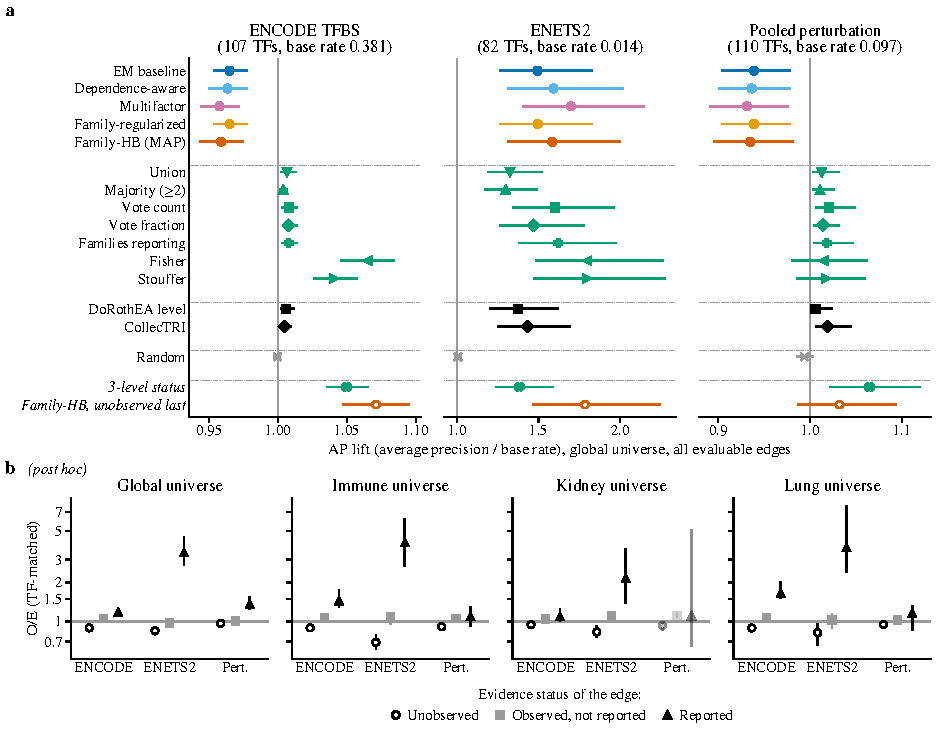
\includegraphics[width=\textwidth]{fig4_heldout.pdf}
  \caption{\textbf{Held-out evaluation in the global universe.} (a) AP lift of every score on all evaluable edges, with 95\% TF-bootstrap intervals; the vertical line marks a random ranking. Open italic rows are post hoc mechanism scores (the 3-level evidence status and Family-HB with unobserved edges ranked last); Family-HB (MAP) is the posterior-mode fit used in the paired tests. Family-HB: ENCODE 0.96 [0.94, 0.98], ENETS2 1.59 [1.31, 2.00], pooled perturbation 0.94 [0.90, 0.98]; Fisher: 1.07 [1.05, 1.08], 1.80 [1.48, 2.27], 1.01 [0.98, 1.06]; EM: 0.96 [0.95, 0.98], 1.49 [1.26, 1.83], 0.94 [0.90, 0.98]. (b) Positives among unobserved, observed but unreported, and reported edges relative to the TF-matched expectation (95\% TF-bootstrap intervals; faded: fewer than 10 TFs with positives or fewer than 20 positives); the whole panel is post hoc. Global universe, unobserved edges: ENCODE 0.89 [0.88, 0.91], ENETS2 0.85 [0.78, 0.90], pooled perturbation 0.97 [0.95, 0.98]; observed negatives 1.05 [1.04, 1.05] (ENCODE). Unobserved edges are depleted of positives in every universe (O/E 0.69 to 0.95 in the tissue universes), whereas the missing-at-random latent-class estimators give them a higher mean credibility than observed negatives (ENCODE-evaluable edges: Family-HB 0.0031 vs 0.00099; EM 0.0068 vs 0.0021): coverage is informative (inference: not missing at random).}
  \label{fig:heldout}
\end{figure}


\paragraph{Why: coverage is not missing at random.}
Over the full universe every latent-class estimator ranks worse than random within TFs on ENCODE and on pooled perturbation data in the global universe (within-TF AUROC \nAucLcmMin{}--\nAucLcmMax{}, every interval below 0.5).
The reason is visible in a post hoc breakdown by the evidence status of edges (\Cref{tab:status}, \Cref{fig:heldout}b).
Relative to the TF-matched expectation, edges that no annotator covers are depleted of held-out positives (observed over expected \nStUnobsEnc{} [\nStUnobsEncLo{}, \nStUnobsEncHi{}] for ENCODE, \nStUnobsEnet{} [\nStUnobsEnetLo{}, \nStUnobsEnetHi{}] for ENETS2, \nStUnobsPert{} [\nStUnobsPertLo{}, \nStUnobsPertHi{}] for perturbation), edges covered but not reported are at expectation (\nStObsnegEnc{}, \nStObsnegEnet{}, \nStObsnegPert{}), and reported edges are enriched (\nStRepEnc{}, \nStRepEnet{}, \nStRepPert{}).
Under the missing-at-random assumption, however, an uncovered edge keeps the prior credibility $w_{\mathrm{T}}$, whereas a covered edge that no annotator reports is pushed below it: Family-HB gives uncovered edges a mean credibility of \nStCredUnobs{} and covered-but-unreported edges \nStCredObsneg{}, the reverse of the held-out ordering.
Fisher and Stouffer avoid the problem only because they give uncovered edges the lowest score.
% provenance: paper/r2/tables/tab_status.tex generated by src/r2/paper_assets on 2026-10-15 04:06 from data/r2/tables/
%   heldout_evidence_status.csv (modified 2026-10-14 20:08): reference in {encode, enets2, pert_pooled}
\begin{table}[tbp]
\centering
\small
\caption{Held-out positive rate by evidence status (post hoc analysis$^{\dagger}$): observed over TF-matched expected positives (O/E, 95\% TF-cluster bootstrap interval) and mean Family-HB credibility $\bar c$ of evaluable edges that no annotator observes, that are observed but not reported, or that carry at least one report.}
\label{tab:status}
\begin{tabular}{@{}lcccccc@{}}
\toprule
Universe & \multicolumn{2}{c}{Unobserved} & \multicolumn{2}{c}{Observed, not reported} & \multicolumn{2}{c}{Reported} \\
\cmidrule(lr){2-3}\cmidrule(lr){4-5}\cmidrule(lr){6-7}
 & O/E & $\bar c$ & O/E & $\bar c$ & O/E & $\bar c$ \\
\midrule
\multicolumn{7}{@{}l}{\emph{ENCODE TFBS}} \\
Global & \begin{tabular}[t]{@{}c@{}}0.89\\[-1pt]{\scriptsize [0.88, 0.91]}\end{tabular} & 0.0031 & \begin{tabular}[t]{@{}c@{}}1.05\\[-1pt]{\scriptsize [1.04, 1.05]}\end{tabular} & $9.9\times 10^{-4}$ & \begin{tabular}[t]{@{}c@{}}1.17\\[-1pt]{\scriptsize [1.11, 1.24]}\end{tabular} & 0.24 \\
Immune & \begin{tabular}[t]{@{}c@{}}0.89\\[-1pt]{\scriptsize [0.87, 0.91]}\end{tabular} & 0.0063 & \begin{tabular}[t]{@{}c@{}}1.07\\[-1pt]{\scriptsize [1.06, 1.09]}\end{tabular} & 0.0015 & \begin{tabular}[t]{@{}c@{}}1.44\\[-1pt]{\scriptsize [1.28, 1.78]}\end{tabular} & 0.26 \\
Kidney & \begin{tabular}[t]{@{}c@{}}0.95\\[-1pt]{\scriptsize [0.93, 0.95]}\end{tabular} & 0.0063 & \begin{tabular}[t]{@{}c@{}}1.05\\[-1pt]{\scriptsize [1.04, 1.06]}\end{tabular} & 0.0015 & \begin{tabular}[t]{@{}c@{}}1.09\\[-1pt]{\scriptsize [1.00, 1.26]}\end{tabular} & 0.26 \\
Lung & \begin{tabular}[t]{@{}c@{}}0.89\\[-1pt]{\scriptsize [0.87, 0.91]}\end{tabular} & 0.0047 & \begin{tabular}[t]{@{}c@{}}1.07\\[-1pt]{\scriptsize [1.05, 1.08]}\end{tabular} & $9.8\times 10^{-4}$ & \begin{tabular}[t]{@{}c@{}}1.65\\[-1pt]{\scriptsize [1.49, 2.02]}\end{tabular} & 0.27 \\
\addlinespace[3pt]
\multicolumn{7}{@{}l}{\emph{ENETS2}} \\
Global & \begin{tabular}[t]{@{}c@{}}0.85\\[-1pt]{\scriptsize [0.78, 0.90]}\end{tabular} & 0.0031 & \begin{tabular}[t]{@{}c@{}}0.98\\[-1pt]{\scriptsize [0.95, 1.01]}\end{tabular} & $9.9\times 10^{-4}$ & \begin{tabular}[t]{@{}c@{}}3.41\\[-1pt]{\scriptsize [2.70, 4.53]}\end{tabular} & 0.25 \\
Immune & \begin{tabular}[t]{@{}c@{}}0.69\\[-1pt]{\scriptsize [0.61, 0.79]}\end{tabular} & 0.0063 & \begin{tabular}[t]{@{}c@{}}1.09\\[-1pt]{\scriptsize [0.95, 1.18]}\end{tabular} & 0.0015 & \begin{tabular}[t]{@{}c@{}}4.05\\[-1pt]{\scriptsize [2.66, 6.21]}\end{tabular} & 0.26 \\
Kidney & \begin{tabular}[t]{@{}c@{}}0.83\\[-1pt]{\scriptsize [0.75, 0.93]}\end{tabular} & 0.0063 & \begin{tabular}[t]{@{}c@{}}1.10\\[-1pt]{\scriptsize [1.01, 1.17]}\end{tabular} & 0.0015 & \begin{tabular}[t]{@{}c@{}}2.15\\[-1pt]{\scriptsize [1.38, 3.63]}\end{tabular} & 0.28 \\
Lung & \begin{tabular}[t]{@{}c@{}}0.82\\[-1pt]{\scriptsize [0.66, 0.96]}\end{tabular} & 0.0047 & \begin{tabular}[t]{@{}c@{}}1.03\\[-1pt]{\scriptsize [0.89, 1.15]}\end{tabular} & $9.7\times 10^{-4}$ & \begin{tabular}[t]{@{}c@{}}3.73\\[-1pt]{\scriptsize [2.39, 7.83]}\end{tabular} & 0.29 \\
\addlinespace[3pt]
\multicolumn{7}{@{}l}{\emph{Pooled perturbation}} \\
Global & \begin{tabular}[t]{@{}c@{}}0.97\\[-1pt]{\scriptsize [0.95, 0.98]}\end{tabular} & 0.0031 & \begin{tabular}[t]{@{}c@{}}1.01\\[-1pt]{\scriptsize [1.00, 1.02]}\end{tabular} & 0.0011 & \begin{tabular}[t]{@{}c@{}}1.36\\[-1pt]{\scriptsize [1.24, 1.56]}\end{tabular} & 0.24 \\
Immune & \begin{tabular}[t]{@{}c@{}}0.91\\[-1pt]{\scriptsize [0.85, 0.95]}\end{tabular} & 0.0063 & \begin{tabular}[t]{@{}c@{}}1.06\\[-1pt]{\scriptsize [1.03, 1.11]}\end{tabular} & 0.0016 & \begin{tabular}[t]{@{}c@{}}1.09\\[-1pt]{\scriptsize [0.92, 1.31]}\end{tabular} & 0.28 \\
Kidney$^{*}$ & \begin{tabular}[t]{@{}c@{}}0.93\\[-1pt]{\scriptsize [0.86, 0.97]}\end{tabular} & 0.0063 & \begin{tabular}[t]{@{}c@{}}1.11\\[-1pt]{\scriptsize [1.07, 1.17]}\end{tabular} & 0.0018 & \begin{tabular}[t]{@{}c@{}}1.10\\[-1pt]{\scriptsize [0.64, 5.09]}\end{tabular} & 0.30 \\
Lung & \begin{tabular}[t]{@{}c@{}}0.95\\[-1pt]{\scriptsize [0.91, 0.98]}\end{tabular} & 0.0047 & \begin{tabular}[t]{@{}c@{}}1.03\\[-1pt]{\scriptsize [1.01, 1.06]}\end{tabular} & $9.2\times 10^{-4}$ & \begin{tabular}[t]{@{}c@{}}1.16\\[-1pt]{\scriptsize [0.86, 1.34]}\end{tabular} & 0.33 \\
\bottomrule
\end{tabular}
\par\smallskip
\begin{minipage}{\linewidth}\footnotesize
$^{*}$\,At least one status group has low support (few positives or TFs).

O/E = 1: positives occur at the rate expected from the TF's own positive rate. $\bar c$: mean posterior-mode credibility of the group.

$^{\dagger}$\,Post hoc: defined after the held-out data had been examined.
\end{minipage}
\end{table}

A post hoc check confirms the mechanism: a label-free score that merely orders uncovered below covered-unreported below reported edges reaches AP lifts of \nApStatusEnc{}, \nApStatusEnet{} and \nApStatusPert{}, and Family-HB with uncovered edges moved to the bottom reaches \nApUlEnc{}, \nApUlEnet{} and \nApUlPert{}, matching Fisher on the ChIP references.
Where the deficit lies depends on the reference and the universe.
On ENCODE it lies within TFs in both metrics (composition-adjusted AP lift \nAdjHbEnc{} against \nAdjFiEnc{} for Fisher; within-TF AUROC \nAucHbEnc{} [\nAucHbEncLo{}, \nAucHbEncHi{}]); on ENETS2 the within-TF deficit relative to mid-$p$ Fisher and Stouffer lies in AP only (within-TF AUROC difference to Fisher \nPairAucFiEnet{} [\nPairAucFiEnetLo{}, \nPairAucFiEnetHi{}]), whereas against EM the within-TF AUROC of Family-HB is slightly lower (\nPairAucEmEnet{} [\nPairAucEmEnetLo{}, \nPairAucEmEnetHi{}], Holm-adjusted bootstrap $p\le\nPairAucEmEnetP{}$, the resampling floor; descriptive).
On pooled perturbation data in the global universe most of the deficit is between-TF composition, although placing uncovered edges last still lifts the within-TF AUROC to random (above).
In the tissue universes, whose perturbation evidence comes from \nTfsPosTisMin{}--\nTfsPosTisMax{} TFs with positives, Family-HB has within-TF perturbation deficits (composition-adjusted AP lift \nAdjHbTisPertMin{}--\nAdjHbTisPertMax{}) that disappear when its uncovered edges are placed last (\nAdjUlTisPertMin{}--\nAdjUlTisPertMax{}), as on ChIP, and within-TF AUROC moves the same way. With so few TFs these comparisons are fragile: bootstrap intervals over so few clusters tend to be too narrow, percentile and normal-approximation bootstrap tests disagree for several of the tissue contrasts, and the coverage of the paired intervals was not checked by simulation.

\paragraph{The head of the ranking.}
The highest-credibility edges do carry held-out support: the \nEvalK{} top-ranked evaluable edges of Family-HB are enriched \nEnrHbEnc{}-fold [\nEnrHbEncLo{}, \nEnrHbEncHi{}] for ENCODE binding, \nEnrHbEnet{}-fold [\nEnrHbEnetLo{}, \nEnrHbEnetHi{}] for ENETS2 and \nEnrHbPert{}-fold [\nEnrHbPertLo{}, \nEnrHbPertHi{}] for perturbation positives, and \nSenrHbEnc{}-, \nSenrHbEnet{}- and \nSenrHbPert{}-fold after stratification by TF and target degree.
Restricted to edges with at least one held-in report, Family-HB is neither the best nor the worst estimator.
In the tissue universes, which contain \nChipTfsTisMin{}--\nChipTfsTisMax{} ChIP-assayed TFs each, Family-HB is below every non-EM comparator on ENCODE (differences \nTisEncDMin{} to \nTisEncDMax{}).
Expression-based network inference sets a sensible bar there, and Family-HB does not reach it.
The predicted sets (\nTopK{} targets per TF) of GRNBoost2 and of absolute Pearson correlation have a higher TF-matched ENCODE enrichment than the predicted set of Family-HB (posterior-mean credibility of the tissue fit) in every tissue: \nPsGbEncImm{} and \nPsPeEncImm{} against \nPsHbEncImm{} in immune, \nPsGbEncKid{} and \nPsPeEncKid{} against \nPsHbEncKid{} in kidney, and \nPsGbEncLung{} and \nPsPeEncLung{} against \nPsHbEncLung{} in lung (post hoc comparison of point estimates; Supplementary Table~\ref{tab:S-fm-heldout}).
On ENETS2 the same holds in immune (\nPsGbEnetImm{} and \nPsPeEnetImm{} against \nPsHbEnetImm{}) and kidney (\nPsGbEnetKid{} and \nPsPeEnetKid{} against \nPsHbEnetKid{}), and in kidney the Family-HB set is not above a random one (ENCODE \nPsHbEncKid{} against \nPsRandEncKid{}, ENETS2 \nPsHbEnetKid{} against \nPsRandEnetKid{}).
This is the coverage failure again: a tissue universe has only \nCtxRepPerTfMin{} to \nCtxRepPerTfMax{} reported edges per TF on average, so most of the \nTopK{} predicted targets of Family-HB are edges without any report, among which uncovered edges are ranked above covered but unreported ones (\Cref{tab:status}). Consistent with this, in a post hoc check the deficit shrinks for predicted sets of \nTopKSensLo{} targets per TF, which contain fewer unreported edges (ENCODE enrichment \nPsHbEncLoKMin{}--\nPsHbEncLoKMax{}; Supplementary Table~\ref{tab:S-fm-sens}).

\emph{Implication.} Fusing references with a latent-class model gives a defensible ranking of the edges the references actually speak to, but not of the universe as a whole. Any use of credibility over a candidate universe must treat uncovered pairs explicitly, which is what claim tiers built on reported edges do (\Cref{sec:res-governance}).


\subsection{Modelling coverage as informative does not repair the ranking}\label{sec:res-obs}

The extension of \Cref{sec:obsmodel}, which lets coverage by literature resources depend on the latent class, was fitted to EM and Family-HB in all universes (Supplementary Tables~\ref{tab:S-obs-fit}--\ref{tab:S-obs-heldout} and Fig.~\ref{fig:S-obs}).
It fails as a generative model.
The observation term contributes \nObsShare{}\% of the joint log-likelihood, and the latent class becomes an attribute of the target gene: \nObsVar{}\% of the variance of the credibility lies between target genes, against \nObsVarHb{}\% for Family-HB.
This happens because a resource's coverage of a pair is the gene's presence in the resource, repeated over every TF the resource covers.
The two models also choose opposite labellings: Family-HB with informative observation assigns the true class to rarely covered genes (class weight \nObsWtHbObs{}), EM with informative observation to frequently covered ones (\nObsWtEmObs{}); each model's label-swapped optimum is the other model's best.
Neither improves the prediction of reports in cross-validation.
On held-out data the Family-HB variant stays below random (ENCODE AP lift \nObsApHbObs{}), and the EM variant is above random (\nObsApEmObs{} [\nObsApEmObsLo{}, \nObsApEmObsHi{}]) but below the label-free status score (\nObsApStatus{}) and Fisher (\nObsApFisher{}); after stratification by TF and target degree its top \nEvalK{} edges carry essentially no enrichment (\nObsSenrEmObs{}), so it acts as a gene-popularity score.
Down-weighting the replicated observation term by the number of eligible TFs removes the degeneracy but returns credibilities nearly identical to Family-HB (Spearman \nObsTfwSp{}) and does not repair the ranking.
In the hub-bias simulation of \Cref{sec:inference} (post hoc), all \nObsSimN{} Family-HB fits with informative observation inflate the true class to \nObsSimWtAllPctMin{}--\nObsSimWtAllPctMax{}\% of the edges (scenario medians \nObsSimWtPctMin{}--\nObsSimWtPctMax{}\%, against a true share of about \nObsSimTruePct{}\%), so the failure is a property of the model rather than of these data.
\emph{Implication:} coverage is informative, but at the level of genes and TFs, not of individual edges, and an edge-level selection model cannot capture it; a gene-level coverage model is a natural next step.

\subsection{Context-matched gains in raw precision are prevalence effects}\label{sec:res-universe}

The perturbation positive rate is higher in every tissue-context universe than in the global universe, so raw precision can be higher there without any better ranking; read naively, such a gain looks like a benefit of matching the candidate universe to the biological context.
\Cref{eq:decomp} separates the two sources (\Cref{tab:decomp}, \Cref{fig:universe}).
In the immune universe the pooled perturbation positive rate is \nUniBaseImm{} against \nUniBaseGlob{} globally, a ratio of \nUniBr{}; the ratio of raw precision among the \nEvalK{} top-ranked edges is \nUniRaw{} [\nUniRawLo{}, \nUniRawHi{}], so the enrichment ratio is \nUniEnr{} [\nUniEnrLo{}, \nUniEnrHi{}]: the context ranking is \emph{less} enriched than the global one, and the whole raw gain is prevalence.
Random sub-universes of the global universe with the context's size and exactly its number of positives give a median precision of \nUniNull{} [\nUniNullLo{}, \nUniNullHi{}] against \nUniCtx{} in the context; \nUniSurvEdge{}\% of the raw gap survives an edge-level null and \nUniSurvBlock{}\% a null that samples whole TF blocks (post hoc; two-sided $p=\nUniPEdge{}$ and \nUniPBlock{}), and for best $F_1$ almost none of it survives (\nUniFOneSurv{}\%).
% provenance: paper/r2/tables/tab_decomp.tex generated by src/r2/paper_assets on 2026-10-15 04:06 from data/r2/tables/
%   heldout_universe_decomposition.csv (modified 2026-10-14 20:08): metric == p_at_500 & credibility == global_fit
%   heldout_downsampling_null.csv (modified 2026-10-14 20:08): metric == p_at_500 & credibility == global_fit & null in {prevalence_matched, tf_block_matched}
\begin{table}[tbp]
\centering
\small
\setlength{\tabcolsep}{4pt}
\caption{Universe-aware decomposition of the context--global difference in raw precision of the top 500 edges (global-fit Family-HB credibility): raw ratio = base-rate ratio $\times$ enrichment ratio, and comparison with prevalence-matched random sub-universes of the global universe drawn edge by edge or as whole TF blocks.}
\label{tab:decomp}
\begin{tabular}{@{}lccccccccc@{}}
\toprule
 & \multicolumn{2}{c}{Base rate} & \multicolumn{3}{c}{P@500} & \multicolumn{2}{c}{Edge null} & \multicolumn{2}{c}{TF-block null$^{\dagger}$} \\
\cmidrule(lr){2-3}\cmidrule(lr){4-6}\cmidrule(lr){7-8}\cmidrule(lr){9-10}
Tissue & Context & Ratio & Context & Raw ratio & Enrichment ratio & Median & Surviving & Median & Surviving \\
\midrule
\multicolumn{10}{@{}l}{\emph{ENCODE TFBS (global universe: P@500 = 0.62, base rate 0.38)}} \\
Immune & 0.24 & 0.62 & 0.41 & \begin{tabular}[t]{@{}c@{}}0.67\\[-1pt]{\scriptsize [0.49, 0.90]}\end{tabular} & \begin{tabular}[t]{@{}c@{}}1.08\\[-1pt]{\scriptsize [0.84, 1.40]}\end{tabular} & \begin{tabular}[t]{@{}c@{}}0.35\\[-1pt]{\scriptsize [0.31, 0.39]}\end{tabular} & $-$0.33 & \begin{tabular}[t]{@{}c@{}}0.32\\[-1pt]{\scriptsize [0.20, 0.49]}\end{tabular} & $-$0.48 \\
Kidney & 0.36 & 0.95 & 0.43 & \begin{tabular}[t]{@{}c@{}}0.69\\[-1pt]{\scriptsize [0.53, 0.88]}\end{tabular} & \begin{tabular}[t]{@{}c@{}}0.72\\[-1pt]{\scriptsize [0.58, 0.92]}\end{tabular} & \begin{tabular}[t]{@{}c@{}}0.48\\[-1pt]{\scriptsize [0.43, 0.52]}\end{tabular} & 0.26 & \begin{tabular}[t]{@{}c@{}}0.43\\[-1pt]{\scriptsize [0.32, 0.59]}\end{tabular} & 0.03 \\
Lung & 0.20 & 0.52 & 0.40 & \begin{tabular}[t]{@{}c@{}}0.65\\[-1pt]{\scriptsize [0.43, 0.87]}\end{tabular} & \begin{tabular}[t]{@{}c@{}}1.26\\[-1pt]{\scriptsize [0.95, 1.59]}\end{tabular} & \begin{tabular}[t]{@{}c@{}}0.28\\[-1pt]{\scriptsize [0.24, 0.32]}\end{tabular} & $-$0.55 & \begin{tabular}[t]{@{}c@{}}0.25\\[-1pt]{\scriptsize [0.17, 0.40]}\end{tabular} & $-$0.69 \\
\addlinespace[3pt]
\multicolumn{10}{@{}l}{\emph{Pooled perturbation (global universe: P@500 = 0.20, base rate 0.10)}} \\
Immune & 0.25 & 2.57 & 0.26 & \begin{tabular}[t]{@{}c@{}}1.28\\[-1pt]{\scriptsize [0.63, 2.51]}\end{tabular} & \begin{tabular}[t]{@{}c@{}}0.50\\[-1pt]{\scriptsize [0.30, 0.80]}\end{tabular} & \begin{tabular}[t]{@{}c@{}}0.25\\[-1pt]{\scriptsize [0.22, 0.27]}\end{tabular} & 0.27 & \begin{tabular}[t]{@{}c@{}}0.25\\[-1pt]{\scriptsize [0.22, 0.32]}\end{tabular} & 0.12 \\
Kidney & 0.15 & 1.55 & 0.14 & \begin{tabular}[t]{@{}c@{}}0.70\\[-1pt]{\scriptsize [0.28, 1.41]}\end{tabular} & \begin{tabular}[t]{@{}c@{}}0.45\\[-1pt]{\scriptsize [0.26, 0.73]}\end{tabular} & \begin{tabular}[t]{@{}c@{}}0.15\\[-1pt]{\scriptsize [0.14, 0.17]}\end{tabular} & 0.19 & \begin{tabular}[t]{@{}c@{}}0.15\\[-1pt]{\scriptsize [0.12, 0.20]}\end{tabular} & 0.19 \\
Lung & 0.29 & 3.04 & 0.29 & \begin{tabular}[t]{@{}c@{}}1.43\\[-1pt]{\scriptsize [0.73, 2.57]}\end{tabular} & \begin{tabular}[t]{@{}c@{}}0.47\\[-1pt]{\scriptsize [0.28, 0.73]}\end{tabular} & \begin{tabular}[t]{@{}c@{}}0.29\\[-1pt]{\scriptsize [0.27, 0.31]}\end{tabular} & 0.02 & \begin{tabular}[t]{@{}c@{}}0.30\\[-1pt]{\scriptsize [0.27, 0.35]}\end{tabular} & $-$0.13 \\
\bottomrule
\end{tabular}
\par\smallskip
\begin{minipage}{\linewidth}\footnotesize
Ratios are context over global. Null: median and 95\% interval of P@500 over random sub-universes with the context's number of evaluable edges and exactly its number of positives, drawn as edges or as whole TF blocks matched to the context's per-TF sizes and positive counts. Surviving: fraction of the context--global gap not reproduced by the null, (context $-$ null median)/(context $-$ global); negative values mean that the context value exceeds its null although raw precision falls. The edge-level null ignores the clustering of edges within TFs and is anti-conservative; the TF-block null keeps it.

Intervals: TF-cluster bootstrap of the context and the global set drawn independently (conservative when the sets share TFs)$^{\dagger}$.

$^{\dagger}$\,Post hoc: defined after the held-out data had been examined.
\end{minipage}
\end{table}

% generated by src/r2/paper_assets (make_paper_assets.py figures); do not edit by hand
% provenance: fig5_universe generated by src/r2/paper_assets on 2026-10-15 04:07 from data/r2/tables/
%   heldout_universe_decomposition.csv (modified 2026-10-14 20:08): metric = p_at_500
%   heldout_downsampling_null.csv (modified 2026-10-14 20:08): metric = p_at_500, null in {prevalence_matched (edge sampling), tf_block_matched (whole TF blocks; post hoc)}
%   (constants): FIG5_K (one of r2.common.PRESPECIFIED['eval_k'])
\begin{figure}[tbp]
  \centering
  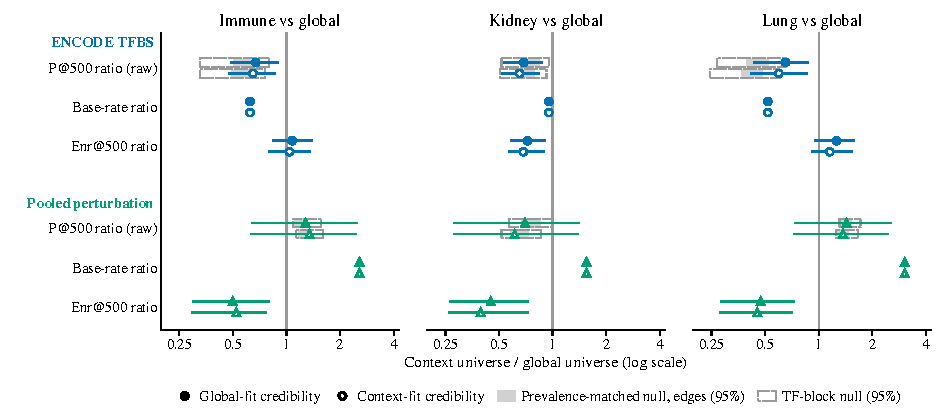
\includegraphics[width=\textwidth]{fig5_universe.pdf}
  \caption{\textbf{Universe-aware decomposition of context-versus-global differences.} For each tissue and reference, the ratio of precision among the 500 highest-credibility evaluable edges in the context universe to that in the global universe (raw P@500 ratio) is the product of the base-rate ratio and the Enr@500 ratio \eqref{eq:decomp}; 95\% intervals (post hoc) combine independent TF bootstraps of the two universes. Filled markers: Family-HB credibility from the global fit; open markers: from the context fit. Grey bars: central 95\% of the raw ratio under the prevalence-matched null (1{,}000 random sub-universes of the global universe with the context's numbers of evaluable edges and positives, sampled as edges); dashed boxes: the same null sampled as whole TF blocks matched to the context's per-TF sizes (post hoc), which keeps the within-TF dependence. Pooled perturbation, global-fit credibility: immune: raw 1.28 = base rate 2.57 $\times$ enrichment 0.50 [0.30, 0.80]; kidney: raw 0.70 = base rate 1.55 $\times$ enrichment 0.45 [0.26, 0.73]; lung: raw 1.43 = base rate 3.04 $\times$ enrichment 0.47 [0.28, 0.73]. On ENCODE the raw immune ratio is 0.67 although the enrichment ratio is 1.08, because the context base rate is lower (0.24 vs 0.38); the context P@500 (0.41) lies outside the edge-level null distribution (median 0.35, two-sided empirical $p=4.0\times 10^{-3}$, post hoc) and inside the TF-block null distribution (median 0.32, $p=0.21$); the edge-level null ignores the clustering of edges within TFs and is anti-conservative.}
  \label{fig:universe}
\end{figure}

In kidney and lung the context ranking is also less enriched than the global one (enrichment ratios \nUniEnrKid{} and \nUniEnrLung{}); raw precision is nominally higher in lung (ratio \nUniRawLung{} [\nUniRawLungLo{}, \nUniRawLungHi{}]) and lower in kidney (\nUniRawKid{} [\nUniRawKidLo{}, \nUniRawKidHi{}]), where the weaker context ranking outweighs the higher prevalence; as in immune, the raw-precision interval includes 1 in lung.
On ENCODE the context and global rankings are not distinguishable after matching TF blocks (post hoc; two-sided $p$ \nUniEncPImm{}, \nUniEncPKid{} and \nUniEncPLung{} for immune, kidney and lung).
\emph{Implication:} precision-type metrics cannot be compared across candidate universes, however the universes are chosen; differences must be reported on a prevalence-free scale and against a matched null.


\subsection{Label-free claim tiers in foundation-model contexts}\label{sec:res-governance}

\paragraph{Tier sizes.}
Dual-universe governance promotes \nGovPromImm{} edges in the immune universe (Strong \nGovStrongImm{}, Moderate \nGovModImm{}), \nGovPromKid{} in kidney and \nGovPromLung{} in lung, \nGovShareMin{}--\nGovShareMax{}\% of each context universe (\Cref{tab:governance}); posterior draws give intervals of \nGovPromImmLo{}--\nGovPromImmHi{}, \nGovPromKidLo{}--\nGovPromKidHi{} and \nGovPromLungLo{}--\nGovPromLungHi{} promoted edges.
The BFDR of the promoted set under the context fit is \nGovBfdrPromMin{}--\nGovBfdrPromMax{}, but that of the Moderate tier alone is \nGovBfdrModMin{}--\nGovBfdrModMax{} under the context fit and \nGovBfdrModGlobMin{}--\nGovBfdrModGlobMax{} under the global fit: between one in three and two in five Moderate claims are expected to be false, and Moderate claims should be read as hypotheses.
The two fits agree moderately on the level of an edge (linearly weighted $\kappa$ \nGovKappaMin{}--\nGovKappaMax{} among edges at least Moderate under either).
% provenance: paper/r2/tables/tab_governance.tex generated by src/r2/paper_assets on 2026-10-15 04:06 from data/r2/tables/
%   gov_tiers.csv (modified 2026-10-14 20:11): scope == dual
%   gov_consistency.csv (modified 2026-10-14 20:11): credibility == nuts & scope in {all_edges, either_ge_moderate}
%   gov_tier_validation.csv (modified 2026-10-14 20:11): tissues: scope == dual & tier == Promoted; global: scope == global_fit & tier in {Strong, Moderate, Promoted}
\begin{table}[tbp]
\centering
\small
\caption{Claim governance. Dual-universe tiers in the tissue-context universes (95\% interval over posterior draws), their posterior expected FDR under the global and the context fit, agreement of the two fits, and held-out enrichment of promoted edges after TF matching (O/E, 95\% TF-cluster bootstrap interval). Global universe: single-fit tiers.}
\label{tab:governance}
\begin{tabular}{@{}lcccc@{}}
\toprule
 & Immune & Kidney & Lung & Global \\
\midrule
\multicolumn{5}{@{}l}{\emph{Tier size (edges)}} \\
Strong & \begin{tabular}[t]{@{}c@{}}297\\[-1pt]{\scriptsize [275, 309]}\end{tabular} & \begin{tabular}[t]{@{}c@{}}149\\[-1pt]{\scriptsize [128, 160]}\end{tabular} & \begin{tabular}[t]{@{}c@{}}204\\[-1pt]{\scriptsize [170, 230]}\end{tabular} & 4{,}060 \\
Moderate & \begin{tabular}[t]{@{}c@{}}196\\[-1pt]{\scriptsize [178, 205]}\end{tabular} & \begin{tabular}[t]{@{}c@{}}127\\[-1pt]{\scriptsize [107, 130]}\end{tabular} & \begin{tabular}[t]{@{}c@{}}208\\[-1pt]{\scriptsize [174, 211]}\end{tabular} & 3{,}274 \\
Conditional & \begin{tabular}[t]{@{}c@{}}73\\[-1pt]{\scriptsize [61, 141]}\end{tabular} & \begin{tabular}[t]{@{}c@{}}56\\[-1pt]{\scriptsize [51, 126]}\end{tabular} & \begin{tabular}[t]{@{}c@{}}63\\[-1pt]{\scriptsize [50, 177]}\end{tabular} & -- \\
Promoted (Strong $\cup$ Moderate) & \begin{tabular}[t]{@{}c@{}}493\\[-1pt]{\scriptsize [456, 512]}\end{tabular} & \begin{tabular}[t]{@{}c@{}}276\\[-1pt]{\scriptsize [237, 289]}\end{tabular} & \begin{tabular}[t]{@{}c@{}}412\\[-1pt]{\scriptsize [344, 434]}\end{tabular} & 7{,}334$^{\dagger}$ \\
\addlinespace[3pt]
\multicolumn{5}{@{}l}{\emph{Posterior expected FDR (global fit / context fit)}} \\
Strong & 0.048 / 0.036 & 0.046 / 0.034 & 0.044 / 0.041 & -- \\
Promoted & 0.190 / 0.159 & 0.195 / 0.157 & 0.191 / 0.167 & -- \\
\addlinespace[3pt]
\multicolumn{5}{@{}l}{\emph{Agreement of global and context fit (linearly weighted $\kappa$)}} \\
All edges & 0.93 & 0.90 & 0.92 & -- \\
Edges $\geq$ Moderate in either fit & 0.67 & 0.58 & 0.64 & -- \\
\addlinespace[3pt]
\multicolumn{5}{@{}l}{\emph{Held-out O/E of promoted edges, TF-matched}} \\
ENCODE TFBS & \begin{tabular}[t]{@{}c@{}}1.67\\[-1pt]{\scriptsize [1.35, 2.38]}\end{tabular} & \begin{tabular}[t]{@{}c@{}}1.24\\[-1pt]{\scriptsize [1.03, 1.81]}\end{tabular} & \begin{tabular}[t]{@{}c@{}}2.27\\[-1pt]{\scriptsize [1.78, 3.37]}\end{tabular} & \begin{tabular}[t]{@{}c@{}}1.26$^{\dagger}$\\[-1pt]{\scriptsize [1.16, 1.43]}\end{tabular} \\
ENETS2 & \begin{tabular}[t]{@{}c@{}}5.95\\[-1pt]{\scriptsize [3.39, 9.05]}\end{tabular} & \begin{tabular}[t]{@{}c@{}}3.66\\[-1pt]{\scriptsize [1.30, 7.65]}\end{tabular} & \begin{tabular}[t]{@{}c@{}}6.74\\[-1pt]{\scriptsize [4.12, 13.83]}\end{tabular} & \begin{tabular}[t]{@{}c@{}}5.29$^{\dagger}$\\[-1pt]{\scriptsize [3.86, 8.13]}\end{tabular} \\
Pooled perturbation & \begin{tabular}[t]{@{}c@{}}1.20\\[-1pt]{\scriptsize [0.82, 1.64]}\end{tabular} & \begin{tabular}[t]{@{}c@{}}0.66$^{*}$\\[-1pt]{\scriptsize [0.00, 1.00]}\end{tabular} & \begin{tabular}[t]{@{}c@{}}1.29$^{*}$\\[-1pt]{\scriptsize [1.13, 1.57]}\end{tabular} & \begin{tabular}[t]{@{}c@{}}1.71$^{\dagger}$\\[-1pt]{\scriptsize [1.45, 2.16]}\end{tabular} \\
\bottomrule
\end{tabular}
\par\smallskip
\begin{minipage}{\linewidth}\footnotesize
$^{*}$\,Few TF clusters among the evaluable promoted edges; interval unreliable.

Single-fit levels: Strong, the largest prefix of whole tie blocks with posterior expected FDR $\leq$ 0.05; Moderate, the largest prefix with $\leq$ 0.20, minus Strong. Dual tiers: Strong if Strong under both fits (the intersection of the two single-fit Strong sets); Moderate if at least Moderate under both, not Strong; Conditional if at least Moderate under exactly one fit. Tiers use posterior-mean credibilities. The global universe has a single fit, so it has no Conditional tier and no cross-universe agreement (--).

$^{\dagger}$\,Post hoc: defined after the held-out data had been examined.
\end{minipage}
\end{table}


\paragraph{Held-out validation.}
After matching on TF, promoted edges are enriched for ENCODE binding (observed over expected \nGovOeEncImm{} [\nGovOeEncImmLo{}, \nGovOeEncImmHi{}] in immune, \nGovOeEncKid{} [\nGovOeEncKidLo{}, \nGovOeEncKidHi{}] in kidney, \nGovOeEncLung{} [\nGovOeEncLungLo{}, \nGovOeEncLungHi{}] in lung) and for ENETS2 edges (\nGovOeEnetImm{}, \nGovOeEnetKid{} and \nGovOeEnetLung{}), and the enrichment declines from the promoted tiers to Exploratory, which holds almost all edges and lies slightly below expectation (ENCODE \nGovExplEncMin{}--\nGovExplEncMax{}, ENETS2 \nGovExplEnetMin{}--\nGovExplEnetMax{}). The decline is not strict tier by tier: in immune the Moderate tier is as enriched for ENCODE binding as the Strong tier, and in kidney none of the \nGovModEnetKidNeval{} ENETS2-evaluable Moderate edges is an ENETS2 positive (\Cref{fig:governance}b).
A one-sided Mantel trend test across the four tiers (a screen, because it treats the edges of a stratum as exchangeable; \Cref{sec:governance}), stratified by TF and target degree, gives Holm-adjusted $p\le \nGovTrendChipMax{}$ for every tissue and ChIP reference; stratified by TF alone it gives $p\le\nGovTrendTfOtherMax{}$ except for kidney, where $p=\nGovTrendTfKidEnc{}$ on ENCODE and \nGovTrendTfKidStrict{} on ENCODE-strict, so the kidney gradient depends on adjusting for target degree.
In the global universe the gradient also appears in perturbation data (Strong \nGovGlobPertStrong{} [\nGovGlobPertStrongLo{}, \nGovGlobPertStrongHi{}], Moderate \nGovGlobPertMod{} [\nGovGlobPertModLo{}, \nGovGlobPertModHi{}], below Moderate \nGovGlobPertBelow{}), and on ENETS2 it is steep (\nGovGlobEnetStrong{}, \nGovGlobEnetMod{}, \nGovGlobEnetBelow{}).
In the tissue universes the perturbation evidence is thin: promoted O/E \nGovOePertImm{} [\nGovOePertImmLo{}, \nGovOePertImmHi{}] in immune (\nGovPertNtfImm{} evaluable TFs), \nGovOePertKid{} [\nGovOePertKidLo{}, \nGovOePertKidHi{}] in kidney and \nGovOePertLung{} [\nGovOePertLungLo{}, \nGovOePertLungHi{}] in lung, the last two from \nGovPertNtfKid{} and \nGovPertNtfLung{} evaluable TFs, too few for reliable bootstrap intervals.
Only the immune result is informative, and it does not support the tiers: its interval excludes the global-universe effect of \nGovPertGlobOe{}, which the immune design had power \nGovPertPowImm{} to detect (a post hoc power calculation from the design margins).
Low power is therefore not the explanation there; the cohorts are K562 and THP-1 cells, unrelated to the tissues, and single TFs dominate the evaluable edges (SPI1 holds \nGovPertTopTfPctMin{}--\nGovPertTopTfPctMax{}\% of them in immune and lung).
Part of the ChIP enrichment passes through literature records that themselves rest on ChIP evidence.
% generated by src/r2/paper_assets (make_paper_assets.py figures); do not edit by hand
% provenance: fig6_governance generated by src/r2/paper_assets on 2026-10-15 04:07 from data/r2/tables/
%   gov_tiers.csv (modified 2026-10-14 20:11): scope = dual, tier in {Strong, Moderate, Conditional}; draw interval columns
%   gov_tier_validation.csv (modified 2026-10-14 20:11): universe = global (scope global_fit) or tissues (scope dual); tier in {Strong, Moderate, Conditional}; reference in {encode, enets2, pert_pooled}
%   gov_promoted_by_method.csv (modified 2026-10-14 20:11): k = 50 (method top-k per TF) and method = all_edges
%   (constants): topk_per_tf from r2.common.PRESPECIFIED; MIN_CLUSTERS from r2.governance
\begin{figure}[tbp]
  \centering
  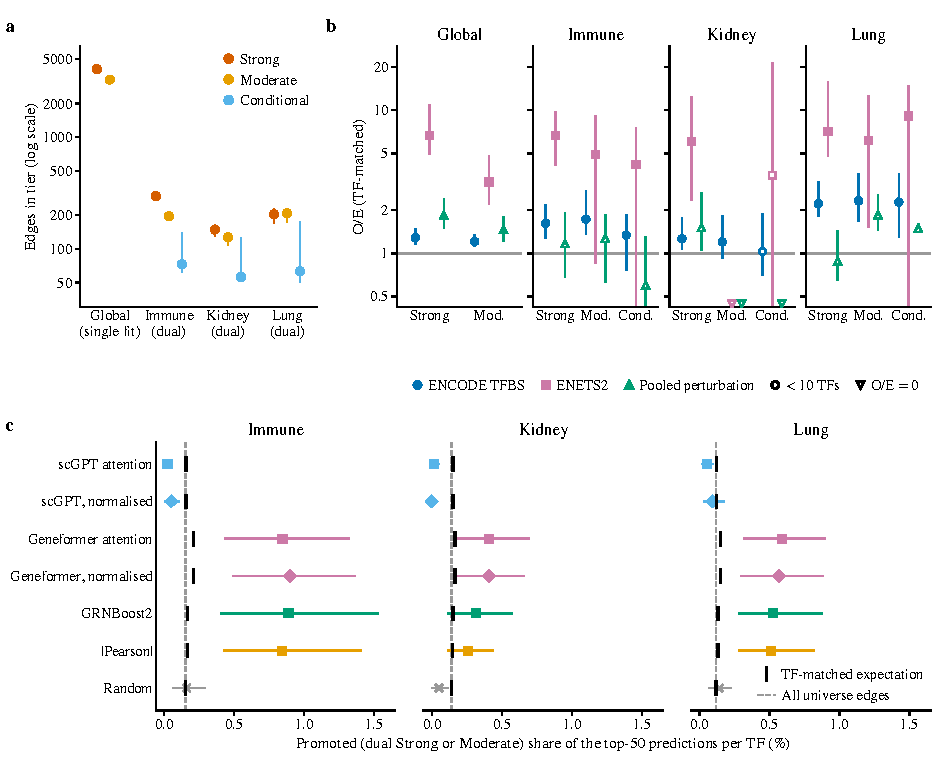
\includegraphics[width=\textwidth]{fig6_governance.pdf}
  \caption{\textbf{Claim governance.} (a) Number of edges per tier: single-fit BFDR tiers in the global universe (Strong 4{,}060, Moderate 3{,}274) and dual-universe tiers in the tissue universes (Strong/Moderate/Conditional: immune 297/196/73; kidney 149/127/56; lung 204/208/63), with 95\% intervals over posterior draws of the credibilities (tissue universes). (b) Held-out positives in each tier relative to the TF-matched expectation, with 95\% TF-bootstrap intervals (open markers: fewer than 10 evaluable TFs; triangles: no positive observed; intervals reaching 0 are cut at the axis). Global universe, Strong tier: ENCODE 1.29 [1.16, 1.48], ENETS2 6.67 [4.88, 10.95], pooled perturbation 1.85 [1.49, 2.43]; Moderate tier: 1.21 [1.11, 1.35], 3.16 [2.21, 4.80], 1.47 [1.21, 1.81]. (c) Share of each method's top-50 predictions per TF that are promoted (95\% TF-bootstrap intervals), against the share expected if the method picked random targets of the same TFs (bars) and the share among all universe edges (dashed). scGPT attention: immune 0.03\% vs 0.16\% expected; Geneformer attention: immune 0.85\% vs 0.21\% expected; GRNBoost2: immune 0.89\% vs 0.17\% expected.}
  \label{fig:governance}
\end{figure}


\paragraph{Foundation-model predictions.}
Almost none of the edges that the foundation models rank highest qualifies as a supported claim (\Cref{tab:methods-promoted}, \Cref{fig:governance}c).
Of the \nMethNpImm{}, \nMethNpKid{} and \nMethNpLung{} scGPT attention predictions (\nTopK{} per TF), \nMethNImm{}, \nMethNKid{} and \nMethNLung{} are promoted, against \nMethExpImm{}, \nMethExpKid{} and \nMethExpLung{} expected from their TFs (exact TF-stratified depletion test, post hoc; $p=\nMethPImm{}$, \nMethPKid{} and \nMethPLung{}).
The exact test treats the edges of a TF as exchangeable and may be anti-conservative: the uniform random score is itself depleted in kidney (\nMethNRandKid{} promoted against \nMethExpRandKid{} expected, $p=\nMethPRandKid{}$), so only the immune depletion is clear-cut.
% provenance: paper/r2/tables/tab_methods_promoted.tex generated by src/r2/paper_assets on 2026-10-15 04:06 from data/r2/tables/
%   gov_promoted_by_method.csv (modified 2026-10-14 20:11): k == 50; method == all_edges (k empty)
\begin{table}[tbp]
\centering
\small
\setlength{\tabcolsep}{4pt}
\caption{Promoted share of each method's predicted set (top 50 targets per TF) in the tissue-context universes, against the share expected from the TF composition of the set (TF-matched expectation); exact one-sided $p$ for enrichment and depletion.}
\label{tab:methods-promoted}
\begin{tabular}{@{}lrrcrccc@{}}
\toprule
Method & Predicted & \multicolumn{2}{c}{Promoted} & Expected & Ratio & \multicolumn{2}{c}{Exact $p$$^{\dagger}$} \\
\cmidrule(lr){3-4}\cmidrule(lr){7-8}
 & edges & $n$ & \% [95\% CI] & \% & & enriched & depleted \\
\midrule
\multicolumn{8}{@{}l}{\emph{Immune}} \\
All edges & 323{,}127 & 493 & 0.15 & 0.15 & 1.00 & -- & -- \\
scGPT & 7{,}900 & 2 & 0.03 [0.00, 0.06] & 0.16 & 0.16 & 1 & $3.5\times 10^{-4}$ \\
scGPT norm. & 7{,}900 & 4 & 0.05 [0.00, 0.11] & 0.16 & 0.33 & 1 & $5.6\times 10^{-3}$ \\
Geneformer & 5{,}322 & 45 & 0.85 [0.43, 1.33] & 0.21 & 4.04 & $2.6\times 10^{-15}$ & 1 \\
Geneformer norm. & 5{,}322 & 48 & 0.90 [0.49, 1.37] & 0.21 & 4.31 & $2.3\times 10^{-17}$ & 1 \\
GRNBoost2 & 7{,}204 & 64 & 0.89 [0.40, 1.53] & 0.17 & 5.28 & $1.7\times 10^{-27}$ & 1 \\
|Pearson| & 7{,}250 & 61 & 0.84 [0.43, 1.41] & 0.17 & 5.03 & $3.8\times 10^{-25}$ & 1 \\
Random & 8{,}050 & 13 & 0.16 [0.06, 0.30] & 0.15 & 1.06 & 0.46 & 0.65 \\
\addlinespace[3pt]
\multicolumn{8}{@{}l}{\emph{Kidney}} \\
All edges & 193{,}686 & 276 & 0.14 & 0.14 & 1.00 & -- & -- \\
scGPT & 5{,}300 & 1 & 0.02 [0.00, 0.06] & 0.15 & 0.12 & 1 & $2.7\times 10^{-3}$ \\
scGPT norm. & 5{,}300 & 0 & 0.00 [0.00, 0.00] & 0.15 & 0.00 & 1 & $2.9\times 10^{-4}$ \\
Geneformer & 4{,}866 & 20 & 0.41 [0.18, 0.70] & 0.17 & 2.49 & $1.9\times 10^{-4}$ & 1 \\
Geneformer norm. & 4{,}866 & 20 & 0.41 [0.18, 0.66] & 0.17 & 2.49 & $1.9\times 10^{-4}$ & 1 \\
GRNBoost2 & 5{,}384 & 17 & 0.32 [0.11, 0.58] & 0.15 & 2.10 & $3.5\times 10^{-3}$ & 1 \\
|Pearson| & 5{,}400 & 14 & 0.26 [0.11, 0.44] & 0.15 & 1.73 & $3.4\times 10^{-2}$ & 0.98 \\
Random & 5{,}700 & 3 & 0.05 [0.00, 0.12] & 0.14 & 0.37 & 0.99 & $3.7\times 10^{-2}$ \\
\addlinespace[3pt]
\multicolumn{8}{@{}l}{\emph{Lung}} \\
All edges & 343{,}512 & 412 & 0.12 & 0.12 & 1.00 & -- & -- \\
scGPT & 7{,}700 & 4 & 0.05 [0.01, 0.10] & 0.12 & 0.43 & 0.98 & $4.5\times 10^{-2}$ \\
scGPT norm. & 7{,}700 & 7 & 0.09 [0.03, 0.18] & 0.12 & 0.76 & 0.82 & 0.29 \\
Geneformer & 5{,}784 & 34 & 0.59 [0.31, 0.90] & 0.15 & 3.88 & $2.8\times 10^{-11}$ & 1 \\
Geneformer norm. & 5{,}784 & 33 & 0.57 [0.29, 0.88] & 0.15 & 3.77 & $1.2\times 10^{-10}$ & 1 \\
GRNBoost2 & 6{,}842 & 36 & 0.53 [0.28, 0.88] & 0.13 & 3.92 & $5.4\times 10^{-12}$ & 1 \\
|Pearson| & 6{,}850 & 35 & 0.51 [0.28, 0.82] & 0.13 & 3.82 & $2.3\times 10^{-11}$ & 1 \\
Random & 7{,}800 & 11 & 0.14 [0.06, 0.23] & 0.12 & 1.18 & 0.34 & 0.77 \\
\bottomrule
\end{tabular}
\par\smallskip
\begin{minipage}{\linewidth}\footnotesize
All universe edges: the whole context universe (reference row; its promoted share is the share of promoted edges in the universe and equals its TF-matched expectation by definition). Interval: 95\% TF-cluster bootstrap interval of the promoted share. Exact $p$: conditional on, for every TF, its numbers of universe, promoted and predicted edges; the test treats the edges of a TF as exchangeable and is anti-conservative when they are dependent.

$^{\dagger}$\,Post hoc: defined after the held-out data had been examined.
\end{minipage}
\end{table}

Geneformer attention and GRNBoost2 predictions are promoted \nMethRatioMinW{} to \nMethRatioMaxW{} times more often than expected from their TFs, but still below \nMethFracBound{}\% of their predictions.
The scGPT attention ranking largely reproduces the attention every target would receive if each cell attended uniformly to its expressed genes: the \nTopK{} top targets per TF overlap with those of this $1/L$ null by \nFmOverlapPctMin{}--\nFmOverlapPctMax{}\%, against \nFmOverlapRandPctMin{}--\nFmOverlapRandPctMax{}\% for a random ranking, and on held-out ENCODE scGPT attention is not enriched beyond the null (post hoc comparison; ratio \nFmEncRatioScMin{}--\nFmEncRatioScMax{}; Supplementary Table~\ref{tab:S-fm-heldout}); on the stricter ENCODE subset it exceeds the null only in kidney (\nFmStrictRatioScKid{} [\nFmStrictRatioScKidLo{}, \nFmStrictRatioScKidHi{}], \nFmStrictScKidTfs{} TFs).
scGPT attention stays below a random score on ENCODE for predicted sets of \nTopKSensLo{}, \nTopK{} and \nTopKSensHi{} targets per TF, and restricting attention to pairs co-observed in at least \nFmMinCoobs{} cells does not remove the null's imprint: the restriction keeps only \nFmCoobsRetPctMin{}--\nFmCoobsRetPctMax{}\% of the scGPT predicted set, and the restricted set still shares \nFmCoobsOvPctMin{}--\nFmCoobsOvPctMax{}\% of its targets with the $1/L$ null, against at most \nFmCoobsOvRandPctMax{}\% for a random ranking (Supplementary Table~\ref{tab:S-fm-sens}).
On the ChIP references and the pooled perturbation reference, Geneformer attention exceeds its null only on ENETS2 (post hoc comparison; ratio \nFmEnetRatioGfImm{} [\nFmEnetRatioGfImmLo{}, \nFmEnetRatioGfImmHi{}] in immune, \nFmEnetRatioGfKid{} in kidney).
\emph{Interpretation:} attention weights of scGPT, extracted as is common practice, reflect how many genes each cell expresses rather than regulatory relationships; Geneformer attention carries a weak signal for the specific ChIP reference.

\paragraph{Sensitivity of the tiers.}
Over the threshold grid (Supplementary Table~\ref{tab:S-gov-grid} and Fig.~\ref{fig:S-gov-grid}) the promoted set grows from \nGovQmImmMin{} to \nGovQmImmMax{} edges in immune as the Moderate threshold moves from \nGovQmGridMin{} to \nGovQmGridMax{}, with stable ENCODE enrichment (\nGovQmOeImmMin{}--\nGovQmOeImmMax{}); the Strong threshold cannot change the promoted set under the primary rule, by construction.
A rule one tier stricter (\Cref{sec:governance}) promotes \nGovStrictImm{}, \nGovStrictKid{} and \nGovStrictLung{} edges; one tier more lenient leaves the promoted set unchanged, because no edge is Strong under one fit and below Moderate under the other.
Posterior-mode instead of posterior-mean credibility changes it little (Jaccard \nGovMapJMin{}--\nGovMapJMax{}).
EM credibility promotes \nGovEmNMin{}--\nGovEmNMax{} edges per tissue.
At equal set size (post hoc), the Family-HB tiers, EM, the number of reporting annotators and the held-in DoRothEA level give overlapping held-out enrichment (ENCODE \nGovSmEncImmMin{}--\nGovSmEncImmMax{} in immune), so what governance adds is an explicit, model-based error statement with posterior uncertainty, not a better ranking.
In the simulations of \Cref{sec:res-fit,sec:res-hubs} that statement is approximately calibrated when the dominant mode is the right one: the realised false discovery rate of the Strong tier is \nSimFdrRightMin{}--\nSimFdrRightMax{} in the mode simulations, against a nominal \nSimClaimed{}.
It is somewhat anti-conservative in the hub simulations without copying (\nSimHbFdrNoCopyMin{}--\nSimHbFdrNoCopyMax{}) and when the class composition depends on literature coverage (\nSimFdrStratImm{} in the immune design with stratum-dependent class weights, \nSimFdrStratGlob{} in the global design), clearly anti-conservative when false claims are copied around hub TFs (\nSimHbFdrCopy{}), and of no help when the wrong mode is selected (\nSimFdrWrong{}).

\paragraph{Concentration.}
The promoted sets concentrate on well-studied TFs: the most frequent TF holds \nGovTopImmPct{}\% (\nGovTopTfImm{}, immune), \nGovTopKidPct{}\% (\nGovTopTfKid{}, kidney) and \nGovTopLungPct{}\% (\nGovTopTfLung{} and SPI1, tied, lung) of the promoted edges, against at most \nGovTopEligBound{}\% of the eligible edges.
A deconcentration operating point chosen without validation data (\nDecBudgetImm{}, \nDecBudgetKid{} and \nDecBudgetLung{} edges, penalty $\lambda=$ \nDecAlphaImm{}, \nDecAlphaKid{} and \nDecAlphaLung{}; its selection rule was fixed after held-out results of other analyses existed) lowers the share of the most frequent TF to \nDecTopPctMin{}--\nDecTopPctMax{}\% while keeping a mean credibility of \nDecCredMin{}--\nDecCredMax{}; its held-out ENCODE enrichment (\nDecOeMin{}--\nDecOeMax{}) rests on \nDecNevalMin{}--\nDecNevalMax{} evaluable edges and is not distinguishable from that of the undeconcentrated set.


\subsection{Hub concentration reflects the evidence, and in simulation modelling dependence reduces it relative to conditional-independence scores}\label{sec:res-hubs}

Is the concentration of promoted edges on hub TFs a property of the estimator or of the evidence? Empirically, \nHubSharePctMin{}--\nHubSharePctMax{}\% of the Family-HB Strong set falls in the top fifth of TFs by literature degree, which holds \nHubPosPctMin{}--\nHubPosPctMax{}\% of the held-out positives, an over-promotion index of \nHubIdxEnc{} [\nHubIdxEncLo{}, \nHubIdxEncHi{}] for ENCODE, \nHubIdxEnet{} [\nHubIdxEnetLo{}, \nHubIdxEnetHi{}] for ENETS2 and \nHubIdxPert{} [\nHubIdxPertLo{}, \nHubIdxPertHi{}] for perturbation (\Cref{fig:hubs}a).
Every estimator and combination rule lies in the same range (\nHubAllMin{}--\nHubAllMax{} for their top \nEvalK{} edges, against \nHubRandMin{}--\nHubRandMax{} for a random score), so the index cannot separate estimators on real data.
% generated by src/r2/paper_assets (make_paper_assets.py figures); do not edit by hand
% provenance: fig7_hubs generated by src/r2/paper_assets on 2026-10-15 04:07 from data/r2/tables/
%   heldout_degree_calibration.csv (modified 2026-10-14 20:08): reference in {encode, enets2, pert_pooled}; (score, set) in (family_hb, strong_bfdr05), (em, top500), (fisher, top500), (dorothea_level_heldin, top500), (random, top500)
%   sim_hub_summary.csv (modified 2026-10-14 20:37): set_rule = size_matched, metric in {over_promotion_lit_q5, over_promotion_top_decile}; methods oracle, family_hb, em, dependence, fisher, stouffer, majority, union, vote_fraction; set_rule = size_matched, metric = set_size, method = family_hb
%   (constants): FEW_TFS from r2.heldout_eval
\begin{figure}[tbp]
  \centering
  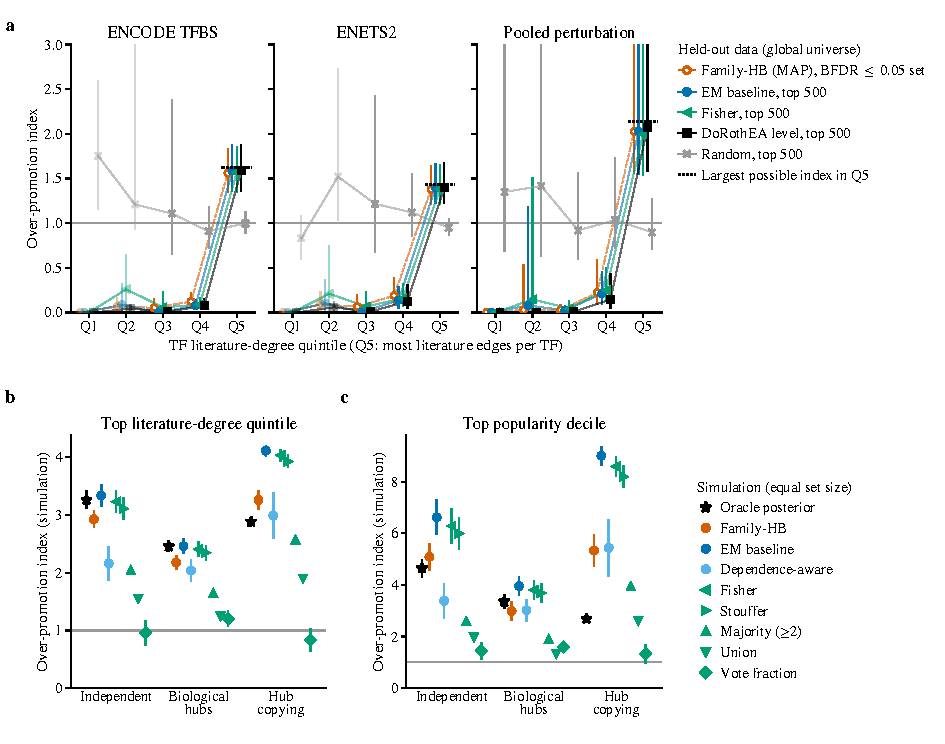
\includegraphics[width=\textwidth]{fig7_hubs.pdf}
  \caption{\textbf{Over-promotion of well-studied TFs.} The over-promotion index of a selected set for a group of TFs is the share of the set in the group divided by the share of positives (a) or of true edges (b, c) in the group (1: proportional to the positives; in (b, c) the oracle posterior shows the level the evidence supports). (a) Held-out data, global universe: index by quintile of TF literature degree for the Family-HB (MAP) BFDR $\leq 0.05$ set and for the top 500 edges of selected scores, with 95\% TF-bootstrap intervals holding the set fixed (faded (post hoc): fewer than 5 evaluable TFs in the quintile). Literature edges per TF in quintiles Q1--Q5: 1--2, 3--6, 7--17, 18--54, 55--1{,}444. The top quintile holds 96\% of the Family-HB set but 62\% of ENCODE positives; index of the Family-HB set in the top quintile: ENCODE 1.56 [1.34, 1.84], ENETS2 1.38 [1.20, 1.65], pooled perturbation 2.03 [1.55, 3.11]; random top 500 on ENCODE: 1.00 [0.88, 1.13]. In the top quintile the index cannot exceed 1/(share of positives) (dotted; ENCODE TFBS 1.62; ENETS2 1.43; Pooled perturbation 2.14), so every informative score is near this ceiling and panel (a) does not separate estimators; the sets also differ in size. (b, c) Simulation with known truth (20 replicates per scenario; mean with 95\% interval over replicates): index of sets of the size of the Family-HB BFDR $\leq 0.05$ set at TFs in the top literature-degree quintile (b) and in the top popularity decile (c), relative to the true edges. Under hub-concentrated copying (b): oracle posterior 2.89 [2.80, 2.97], Family-HB 3.26 [3.10, 3.42], EM 4.11 [4.02, 4.20], Fisher 4.03 [3.93, 4.14]. Family-regularized coincides with EM to two decimals and is not shown. All simulation rows are post hoc.}
  \label{fig:hubs}
\end{figure}

With known truth (the hub-bias simulation of \Cref{sec:inference}, \nSimHubNrep{} replicates per scenario; post hoc) even the posterior of the true generative model concentrates on popular TFs, because true edges of little-studied TFs are rarely reported: for sets of the size of the Family-HB Strong set its over-promotion index is \nSimOrIdxQMin{}--\nSimOrIdxQMax{} in the top literature-degree quintile (\Cref{fig:hubs}b) and \nSimOrIdxMin{}--\nSimOrIdxMax{} in the top popularity decile (\Cref{fig:hubs}c, Supplementary Table~\ref{tab:S-simhub}).
At equal set size, Family-HB is slightly less hub-concentrated than this oracle on the quintile scale, which is the scale of the real-data index, when popular TFs are also biologically more connected (\nSimHbOrQBio{} [\nSimHbOrQBioLo{}, \nSimHbOrQBioHi{}]) or when nothing distinguishes popular TFs (\nSimHbOrQNull{} [\nSimHbOrQNullLo{}, \nSimHbOrQNullHi{}]), and more concentrated when false literature claims are copied preferentially around popular TFs ($+$\nSimHbOrQCopy{} [\nSimHbOrQCopyLo{}, \nSimHbOrQCopyHi{}]).
In the top popularity decile the copying effect is much larger ($+$\nSimHbOrCopy{} [\nSimHbOrCopyLo{}, \nSimHbOrCopyHi{}], against \nSimHbOrBio{} [\nSimHbOrBioLo{}, \nSimHbOrBioHi{}] and $+$\nSimHbOrNull{} [\nSimHbOrNullLo{}, \nSimHbOrNullHi{}] in the other two scenarios); under copying the realised false discovery rate of the Family-HB Strong set rises to \nSimHbFdrCopy{} [\nSimHbFdrCopyLo{}, \nSimHbFdrCopyHi{}], with \nSimHbFpTopCopyPct{}\% of its false claims at top-decile TFs.
The conditional-independence scores are more hub-concentrated than Family-HB: EM and Fisher in all \nSimHubRepAll{} replicates of the three scenarios (top-decile index relative to Family-HB, EM $+$\nSimEmHbMin{} to $+$\nSimEmHbMax{}; Fisher $+$\nSimFiHbMin{} to $+$\nSimFiHbMax{}) and Stouffer in \nSimStGtN{} of them ($+$\nSimStHbMin{} to $+$\nSimStHbMax{}).
The counting rules, union, majority and vote fraction, are less hub-concentrated than Family-HB in every scenario (\nSimCountHbMin{} to \nSimCountHbMax{}), but their precision is lower by \nSimCountPrecLossMin{} to \nSimCountPrecLossMax{}, so their lower concentration reflects a less selective ranking rather than a better one.
\emph{Implication:} hub concentration is largely a consequence of how evidence is generated; in simulation, modelling within-family dependence reduces it relative to the conditional-independence scores, but no reference-only estimator removes it, and promoted edges of hub TFs should be interpreted with that in mind. The simulation uses one generator, whose burst structure resembles Family-HB, so these comparisons are indicative.


\subsection{Cross-cohort replication check}\label{sec:res-replication}

\nRepNEvalCap{} of the \nCohStudies{} perturbation studies are evaluable for TF--target edges in the global universe; Adamson perturbed no TF of the universe and Shifrut had no evaluable positives (\Cref{tab:replication}, \Cref{fig:replication}).
The power calculation fixed before any replication outcome was computed classifies Norman, Papalexi and Replogle as adequately powered (power at a \nRepTrueEnrFold{} enrichment \nRepPowMin{}--\nRepPowMax{}; minimum detectable enrichment \nRepMdeMin{}--\nRepMdeMax{}) and Dixit as underpowered and uninformative (\nRepDixitNpos{} positives; power \nRepDixitPow{}; no number of promoted edges reaches the support floor).
Within TFs, promoted edges are more often perturbation positives than other evaluable edges: stratified enrichment \nRepEnrNorman{} [\nRepEnrNormanLo{}, \nRepEnrNormanHi{}] for Norman, \nRepEnrPapalexi{} [\nRepEnrPapalexiLo{}, \nRepEnrPapalexiHi{}] for Papalexi and \nRepEnrReplogle{} [\nRepEnrReplogleLo{}, \nRepEnrReplogleHi{}] for Replogle (exact stratified $p=\nRepPNorman{}$, \nRepPPapalexi{} and \nRepPReplogle{}), and none for Dixit.
% provenance: paper/r2/tables/tab_replication.tex generated by src/r2/paper_assets on 2026-10-15 04:06 from data/r2/tables/
%   rep_units.csv (modified 2026-10-14 20:15): universe == global & level == study & comparator == universe
%   rep_power.csv (modified 2026-10-08 17:40): universe == global & level == study & comparator == universe
%   rep_pass_rates.csv (modified 2026-10-14 20:15): universe == global & level == study & comparator == universe
%   eval_analysis_decisions.csv (modified 2026-10-15 01:28): module == replication, id == rep_attainable; module == replication, id == rep_wrongtf; module == replication, id == rep_responsiveness; module == replication, id == rep_boot_clusters
%   replication.py.csv: MIN_BOOT_CLUSTERS (TFs needed for a bootstrap interval)
\begin{table}[tbp]
\centering
\small
\setlength{\tabcolsep}{2.4pt}
\caption{Cross-cohort replication check in the global universe, per independent study (Dixit 2016, \citet{dixit2016perturb}; Adamson 2016, \citet{adamson2016multiplexed}; Shifrut 2018, \citet{shifrut2018genome}; Norman 2019, \citet{norman2019exploring}; Papalexi 2021, \citet{papalexi2021characterizing}; Replogle 2022, \citet{replogle2022mapping}). Design quantities were computed and locked before any replication outcome: power of the exact stratified test against a 2-fold enrichment, minimum detectable enrichment (MDE) and support floor (promoted evaluable edges for 80\% power). Outcome: stratified O/E with 95\% TF-cluster bootstrap interval, Mantel--Haenszel odds ratio and exact one-sided $p$.}
\label{tab:replication}
\begin{tabular}{@{}lrrrrrcrclrr@{}}
\toprule
Study & Promoted & \multicolumn{3}{c}{Design (locked)} & Margins & \multicolumn{4}{c}{Outcome} & \multicolumn{2}{c}{Controls (O/E)} \\
\cmidrule(lr){3-5}\cmidrule(lr){6-6}\cmidrule(lr){7-10}\cmidrule(lr){11-12}
 & evaluable & Power & MDE & Floor & Max. & O/E & MH & $p$ & Result & Wrong & Resp.- \\
 & edges & & & & O/E$^{\dagger}$ & [95\% CI]$^{\dagger}$ & OR & & & TF$^{\dagger}$ & strat.$^{\dagger}$ \\
\midrule
Dixit 2016 & 364 & 0.03 & 27.40 & $\infty$ & 136.47 & \begin{tabular}[t]{@{}c@{}}0.00\\[-1pt]{\scriptsize --}\end{tabular} & 0.00 & 1 & \begin{tabular}[t]{@{}l@{}}under-\\powered\end{tabular} & 5.80 & 0.00 \\
Adamson 2016 & 0 & \multicolumn{10}{l}{\emph{non-evaluable: no perturbed TF of the universe tested}} \\
Shifrut 2018 & 8 & \multicolumn{10}{l}{\emph{non-evaluable: no evaluable TF positives}} \\
Norman 2019 & 220 & 1.00 & 1.39 & 40 & 4.28 & \begin{tabular}[t]{@{}c@{}}1.95\\[-1pt]{\scriptsize [1.64, 2.45]}\end{tabular} & 3.27 & $1.9\times 10^{-14}$ & pass & 1.55 & 1.25 \\
Papalexi 2021 & 571 & 1.00 & 1.41 & 109 & 7.50 & \begin{tabular}[t]{@{}c@{}}2.24\\[-1pt]{\scriptsize [1.72, 4.86]}\end{tabular} & 3.64 & $3.1\times 10^{-16}$ & pass & 1.40 & 1.41 \\
Replogle 2022 & 536 & 0.99 & 1.56 & 184 & 12.06 & \begin{tabular}[t]{@{}c@{}}1.57\\[-1pt]{\scriptsize [1.12, 4.86]}\end{tabular} & 2.07 & $7.1\times 10^{-4}$ & pass & 1.18 & 1.34 \\
\bottomrule
\end{tabular}
\par\smallskip
\begin{minipage}{\linewidth}\footnotesize
Pass (O/E $\geq$ 1.5 and $p \leq$ 0.05): 3 of 4 evaluable studies (Wilson 95\% CI 0.30--0.95; a study below its support floor is reported as underpowered, not as a failure, but counts as not passing in this rate); 3 of 3 adequately powered studies (0.44--1.00).

Intervals$^{\dagger}$: TF-cluster bootstrap within the study, given only for studies with at least 5 TFs; --, no interval: fewer TFs, or every resample gives the same O/E (Dixit 2016).

Exact $p$: one-sided exact test conditional on the margins of every (cohort, TF) stratum; it treats the edges of a stratum as exchangeable and is anti-conservative when targets of one TF are dependent, so the TF-cluster bootstrap intervals carry the inference.

Floor $\infty$: no number of promoted edges reaches the target power. Max.\ O/E: largest O/E the margins allow. Wrong-TF: O/E when each promoted edge is scored against the perturbation of a different TF of the same cohort (specificity control). Resp.-strat.: O/E with strata additionally defined by target responsiveness (share of perturbations in which the target responds).

$^{\dagger}$\,Post hoc: defined after the held-out data had been examined.
\end{minipage}
\end{table}

The exact test conditions on the (cohort, TF) strata and treats the target genes within a stratum as exchangeable; targets of one TF are not independent, so these $p$-values are anti-conservative and serve as a screen, while the TF-cluster bootstrap intervals carry the inference.
\nRepPassAllNCap{} of \nRepPassAllD{} evaluable studies pass the endpoint (Wilson interval [\nRepPassAllLo{}, \nRepPassAllHi{}]); the fourth, Dixit, is reported as underpowered rather than as a failure, but it stays in the denominator of this rate, and \nRepPassPowN{} of \nRepPassPowD{} adequately powered studies pass ([\nRepPassPowLo{}, \nRepPassPowHi{}]).
Dropping the most influential TF leaves enrichments of \nRepDropTopMin{}--\nRepDropTopMax{}.
% generated by src/r2/paper_assets (make_paper_assets.py figures); do not edit by hand
% provenance: fig8_replication generated by src/r2/paper_assets on 2026-10-15 04:07 from data/r2/tables/
%   rep_units.csv (modified 2026-10-14 20:15): level = study, comparator = universe, status = evaluable
%   rep_prior_sensitivity.csv (modified 2026-10-14 20:18): level = study, parameter in {mu, theta_new}
%   rep_pass_rates.csv (modified 2026-10-14 20:15): level = study, comparator = universe, subset in {all_evaluable, adequately_powered}
%   rep_power.csv (modified 2026-10-08 17:40): level = study, comparator = universe: alpha, true_enrichment, target_power
%   eval_analysis_decisions.csv (modified 2026-10-15 01:28): module = replication: status of rep_attainable, rep_boot_clusters
%   (constants): replication_endpoint_enrichment from r2.common.PRESPECIFIED; MIN_BOOT_CLUSTERS from r2.replication
\begin{figure}[tbp]
  \centering
  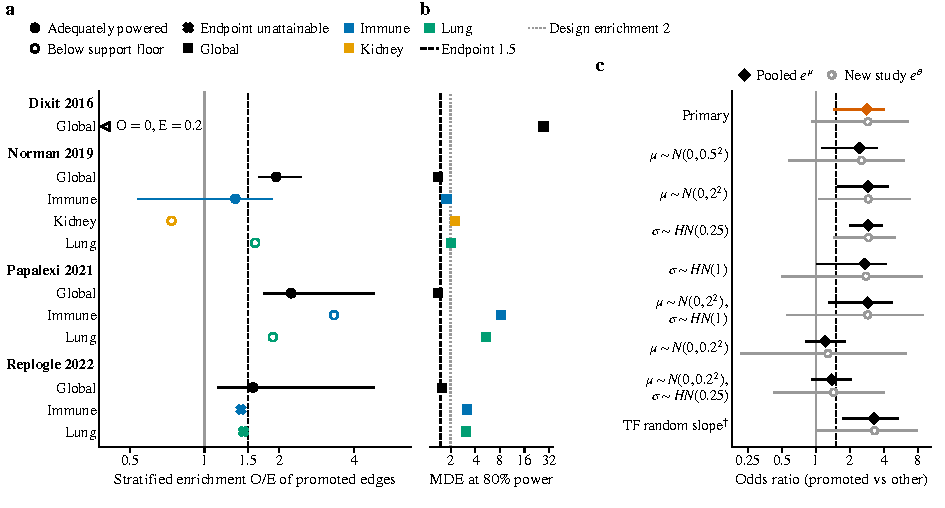
\includegraphics[width=\textwidth]{fig8_replication.pdf}
  \caption{\textbf{Cross-cohort replication check.} (a) Stratified enrichment (observed over TF-stratified expected perturbation positives among promoted evaluable edges) per study and universe (global universe primary, tissue universes secondary), with 95\% TF-bootstrap intervals where at least 5 TFs contribute (post hoc rule); intervals reaching 0 are cut at the axis. Marker shape gives the power class locked before any replication outcome was computed (filled: adequately powered; open: below the support floor); the endpoint-unattainable class (X; the positive-rate margins cannot reach the endpoint) was added post hoc; dashed line: endpoint 1.5 (non-evaluable studies omitted). Global universe: Dixit 2016: 0 observed vs 0.2 expected promoted positives (power 0.03, MDE 27.4); Norman 2019 1.95 [1.64, 2.45] (power 1.00, MDE 1.39); Papalexi 2021 2.24 [1.72, 4.86] (power 1.00, MDE 1.41); Replogle 2022 1.57 [1.12, 4.86] (power 0.99, MDE 1.56). Pass rate 3/4 evaluable studies (a study below the support floor is reported as underpowered but counts as not passing) and 3/3 adequately powered studies. (b) Minimum detectable enrichment at 80\% power and one-sided $\alpha=0.05$ from the design alone (dotted: design enrichment 2). (c) Pooled within-TF odds ratio $e^{\mu}$ and the predicted odds ratio of a new study in the Bayesian random-effects model under the primary and 7 alternative prior specifications and a model with a TF-level random slope$^{\dagger}$ (median and 95\% credible interval; N, normal; HN, half-normal; $^{\dagger}$post hoc). Primary prior: 2.82 [1.42, 4.09], $P(e^{\mu}\geq 1.5)=0.97$; sceptical prior $\mu\sim N(0,0.2^2)$: 1.21 [0.81, 1.81], $P=0.15$; across the alternative priors $P(e^{\mu}\geq 1.5)$ ranges from 0.15 to 0.99; TF random slope: 3.28 [1.71, 5.42], $P=0.99$.}
  \label{fig:replication}
\end{figure}


The check is weaker than these numbers suggest.
Promoted targets are genes that respond to many perturbations: stratifying additionally by how many other perturbed TFs a target responds to lowers the enrichments to \nRepRespNorman{}, \nRepRespPapalexi{} and \nRepRespReplogle{}, and scoring promoted targets against the responses to \emph{other} TFs already gives \nRepWrongNorman{}, \nRepWrongPapalexi{} and \nRepWrongReplogle{}, so the TF-specific excess is \nRepSpecMin{}--\nRepSpecMax{} (post hoc analyses).
After the response stratification all \nRepPassPowN{} remain below the nominal level (exact $p\le\nRepRespPMax{}$), but none reaches the endpoint of \nRepEndpoint{}.
Pooled across studies in the random-effects model, the within-TF odds ratio is \nRepMu{} [\nRepMuLo{}, \nRepMuHi{}] under the primary prior, with probability \nRepPmu{} of exceeding \nRepEndpoint{}, but the predictive interval for a new study is wide (\nRepNewLo{}--\nRepNewHi{}) and a sceptical prior centred on no effect gives \nRepSkept{} [\nRepSkeptLo{}, \nRepSkeptHi{}] (probability \nRepSkeptP{}; Supplementary Table~\ref{tab:S-rep-prior}).
Leave-$k$-out refits show the dependence on individual studies: removing one, two or three studies changes $\mu$ by \nRepLkMeanOne{}, \nRepLkMeanTwo{} and \nRepLkMeanThree{} on average (at most \nRepLkMaxOne{}, \nRepLkMaxTwo{} and \nRepLkMaxThree{}); with three studies removed a single study remains, so the last figures are single-study estimates shrunk towards the prior rather than pooled ones.
A support threshold chosen from the outcomes instead of the power calculation would be unstable: re-estimated leaving one study out, it classifies the left-out study correctly in \nRepTau{} of the cases.
\emph{Interpretation:} with \nRepPassPowD{} adequately powered studies, two of them in K562 cells, the check supports a modest, TF-specific association between promotion and perturbation response; it is not a validation.


\subsection{Sensitivity analyses and the cost of tuning on evaluation data}\label{sec:res-sensitivity}

\paragraph{Priors, evidence variants and family definitions.}
Halving or doubling the hierarchical scale priors and changing the Dirichlet concentration leave the Strong set essentially unchanged (Jaccard at least \nSensPriorMin{}; Supplementary Table~\ref{tab:S-sens-fit}).
The evidence variants matter in a structured way.
The curated-conditional variants agree with the primary (Jaccard \nSensVarKeepMin{}--\nSensVarKeepMax{}) except the panel in which the two most overlapping text-mining annotators, ExTRI and NTNU.Curated, are merged (\nSensVarMergedGlob{} global, \nSensVarMergedImm{} immune), which removes much of the co-reporting that the literature burst explains; adding the ChIP family leaves the Strong set largely unchanged (\nSensVarChipMin{}--\nSensVarChipMax{}).
Treating motif and coexpression annotators as genome-wide or requiring both endpoints, without the condition of literature support, changes the Strong set substantially (\nSensVarLeakMin{}--\nSensVarLeakMax{}) and raises held-out AP lift on ENETS2 by \nHsVarMaskMin{}--\nHsVarMaskMax{}.
Under these masks the fit sees motif and coexpression reports on edges without literature support, which in the distributed data exist only where a held-out ChIP resource supports the edge (\Cref{sec:data-annotators}), and it counts a different set of edges as uncovered; the two explanations are not separated here, and the curated-conditional model excludes both.
The family definition matters most for the size of the Strong set: grouping annotators by integrator lineage keeps \nSensGrpLinKeepPctMin{}--\nSensGrpLinKeepPctMax{}\% of the primary Strong edges but adds about as many again (a set \nSensGrpLinSizeMin{}--\nSensGrpLinSizeMax{} times as large; Jaccard index \nSensGrpLinJacMin{}--\nSensGrpLinJacMax{}), and treating every annotator as its own family removes all burst classes and reproduces the EM result, a set \nSensGrpSingSizeMin{}--\nSensGrpSingSizeMax{} times as large that contains \nSensGrpSingKeepPctMin{}--\nSensGrpSingKeepPctMax{}\% of the primary Strong edges (Jaccard \nSensGrpSingMin{}--\nSensGrpSingMax{}).
The primary Strong set is thus close to a core that every grouping retains, and the grouping decides mainly how many further edges are added.
Clustering annotators by their co-reporting pattern (post hoc) recovers the modality families exactly in the immune universe and up to one literature annotator in the global universe, where ORegAnno joins the motif cluster (adjusted Rand index \nGrpAriFullGlob{}); the Strong sets agree with the primary (Jaccard \nSensGrpDdMin{}--\nSensGrpDdMax{}), but the partition is only partly stable under resampling (mean adjusted Rand index \nGrpAriMin{}--\nGrpAriMax{} over cross-validation training folds and TF bootstraps).
On held-out data none of these choices changes the global ENETS2 AP lift by more than \nHsMaxNonLeak{}, except the two masks without the literature condition and the fit that includes the ChIP family.

\paragraph{Tuning on evaluation labels.}
Every model and evidence choice of the primary analysis was made without validation labels; to quantify what tuning on such labels would have done, we selected among \nTuneNConfigs{} configurations by perturbation AP lift on random halves of the perturbed TFs (Supplementary Table~\ref{tab:S-tuning}).
Within the hyperparameter grid and across random halves of the TFs, tuning gains nothing that transfers: \nTuneNwin{} different configurations win, and the in-sample gain over Family-HB (\nTuneIn{}) disappears on the held-out TFs (\nTuneOut{} [\nTuneOutLo{}, \nTuneOutHi{}]); with a criterion normalised for TF composition (post hoc) a gain of \nTuneNullOut{} remains, positive in \nTuneNullFracPct{}\% of the halves, so the configurations differ very little rather than not at all.
Across studies the picture differs: leaving one study out, the configuration tuned on the other studies beats Family-HB on the left-out study in all \nTuneLosoHbNfold{} folds (mean gain \nTuneLosoHbOut{}), mostly through the Dixit fold (\nTuneLosoHbExcl{} without it; post hoc subset), so label tuning on this grid can transfer between studies, although with \nTuneLosoHbNfold{} folds this is weak evidence.
Over the full grid the tuned choice is the both-endpoints observation rule in \nTuneAllFreqPct{}\% of the halves and retains \nTuneAllRetPct{}\% of its gain, partly through TF composition; across studies it retains \nTuneLosoPct{}\% of its gain, or all of it once the uninformative Dixit fold is dropped.
Choosing by cross-validated likelihood, without any label, reproduces the held-out performance of the primary model (difference \nTuneLf{}).
A selection objective that weighs dropout robustness against the perturbation reward depends on its weights and on the robustness metric: it never selects Family-HB with the $F_1$-based metric or when the combination rules are candidates, and selects it at \nTuneJointHbPrecPct{}\% of the weight settings with the precision-based metric among the latent-class models alone (Supplementary Table~\ref{tab:S-tune-weights}).

\subsection{Computation}\label{sec:res-compute}

All statistical analyses ran on one laptop (Apple M2 Pro, \nHwCores{} cores, \nHwRamGiB{}~GiB; \Cref{tab:compute}); the attention matrices were extracted beforehand, and that step is not included.
Pattern compression makes the cost of one likelihood evaluation independent of the number of edges: the \nScNRealMio{} million global edges compress to about \nScPRealApprox{} patterns in about \nScCompRealW{} second, and one evaluation of the log posterior and its gradient takes \nScVgRealMs{}~ms.
One command regenerates every table, figure and number of this paper from the stored fits in \nPipeTablesMin{}~min with at most \nPipeTablesPeakGiB{}~GiB of memory.
A full rebuild from the public inputs took about \nPipeFullHours{}~h of compute as recorded on a machine shared with other jobs, most of it in model fitting and simulation (\Cref{tab:compute}); \nPipeRecordedPct{}\% of that time consists of recorded runtimes of the original runs, and isolated re-runs of the dominant steps are \nPipeIsoRatioMin{} to \nPipeIsoRatioMax{} times faster, so the figure describes the runs as made rather than the cost on an idle machine.
As recorded, the Family-HB posterior-mode fit with \nMapRestartsHb{} restarts took \nRtMapGlob{}~s for the global universe and \nRtMapTisMin{}--\nRtMapTisMax{}~s for each tissue, and the dominant-mode NUTS fit took \nRtNutsGlobMinutes{}~min for the global universe and \nRtNutsTisMinutesMin{}--\nRtNutsTisMinutesMax{}~min for the tissues; re-run one at a time, all posterior-mode fits of the five estimators in the four universes took \nPipeMapIsoS{}~s together, and the kidney NUTS fit \nPipeNutsKidIsoMin{}~min.
In synthetic universes ten times larger (a post hoc experiment) the number of patterns grows sublinearly (exponent \nScPN{} in the number of edges), and the posterior-mode fit remains feasible: with \nScMapRestarts{} restarts it takes \nScMapTenKOne{}~s with \nScKOne{} annotators and about \nScMapTenKTwoHours{}~h (projected) with \nScKTwo{}, or about \nScMapFiftyKOneHours{}~h and \nScMapFiftyKTwoHours{}~h with the \nMapRestartsHb{} restarts used for Family-HB here.
Full NUTS becomes expensive: \nScNutsChains{} chains of \nScNutsWarm{} warm-up and \nScNutsDraw{} retained iterations are projected to take \nScNutsKOneLoHours{}--\nScNutsKOneHiHours{}~h with \nScKOne{} annotators and \nScNutsKTwoLoHours{}--\nScNutsKTwoHiHours{}~h with \nScKTwo{} (from the step-count projection, a lower bound, to the projection at the tree-depth cap; \Cref{tab:compute-scaling}), and the \nNutsChains{} chains of \nNutsWarmup{} + \nNutsDraws{} iterations used here at least \nScNutsProdMinHours{}~h, so for larger problems posterior-mode inference with Laplace or bridge-sampling summaries is the practical choice.

% provenance: paper/r2/tables/tab_compute.tex generated by src/r2/paper_assets on 2026-10-15 04:07 from data/r2/tables/
%   scale_summary.csv (modified 2026-10-14 20:38): generator in {template, independent, stress}, selected configurations
%   scale_nuts.csv (modified 2026-10-14 20:38): cid == template_real_K21 (run settings); status == projected (range over sessions)
%   fit_convergence.csv (modified 2026-10-14 19:28): universe == global & fit_id == family_hb_nuts (production NUTS run)
%   scale_environment.csv (modified 2026-10-14 20:38): keys cpu, hw.ncpu, hw.memsize (bytes)
%   pipeline_stage_timings.csv (modified 2026-10-15 04:07): selected == True; summed per stage and mode; fit_primary map and kidney NUTS: recorded vs measured wall time
%   pipeline_environment.csv (modified 2026-10-15 04:06): keys cpu, hw.ncpu, hw.memsize (bytes)
\begin{table}[tbp]
\centering
\small
\setlength{\tabcolsep}{5pt}
\caption{Wall time and peak resident memory of each stage of the analysis pipeline on the real data on one laptop (Apple M2 Pro, 10 cores, 32\,GiB), run through the single entry point \texttt{reproduce\_all.py}. Full run: every step of the stage; tables-only: the steps that regenerate the tables from the stored fits and outputs. Steps marked M were measured as isolated runs, one step process at a time with two threads; steps marked R or L are the runtimes recorded when the long fits originally ran, partly in parallel and with other thread settings on the shared machine, and make up 98\% of the full-run time. The 1-min load average of the machine (other users' jobs included) ranged 3.2--9.3 during the measured steps. Synthetic scaling: Table~\ref{tab:compute-scaling}.}
\label{tab:compute}
\begin{tabular}{@{}lrrlrr@{}}
\toprule
 & \multicolumn{3}{c}{Full run} & \multicolumn{2}{c}{Tables only} \\
\cmidrule(lr){2-4}\cmidrule(lr){5-6}
Stage & min & GiB & timing & min & GiB \\
\midrule
\multicolumn{6}{@{}l}{\emph{Data layer}} \\
Gene panels & 0.028 & 0.15 & M & 0.0068 & 0.11 \\
Annotators (committed inputs) & 0.17 & 1.6 & M & 0.17 & 1.6 \\
Evidence patterns & 0.25 & 0.99 & M & 0.25 & 0.99 \\
GRNBoost2 / GENIE3 & 71 & 5.0 & R & 0.024 & 0.21 \\
Method scores & 0.79 & 2.4 & M & 0.014 & 0.16 \\
Perturbation cohorts & 1.9 & 9.6 & R & 0.033 & 0.41 \\
Held-out ChIP & 0.84 & 4.3 & M & 0.013 & 0.15 \\
\addlinespace[3pt]
\multicolumn{6}{@{}l}{\emph{Model layer}} \\
Primary fits (MAP, NUTS) & 511 & 2.3$^{b}$ & M+R$^{a}$ & 0.16 & 0.31 \\
Sensitivity, CV, PPC, recovery & 657 & 2.0$^{b}$ & L+M+R & 0.53 & 2.0 \\
Informative-observation fits & 603 & -- & L+R$^{a}$ & -- & -- \\
Posterior modes (fits, bridge, simulation) & 688 & -- & L+R & -- & -- \\
\addlinespace[3pt]
\multicolumn{6}{@{}l}{\emph{Evaluation}} \\
Dropout robustness & 323 & 1.6$^{b}$ & L+M+R & 3.1 & 1.6 \\
Held-out evaluation & 39 & 6.6 & M & 39 & 6.6 \\
Claim governance & 0.68 & 2.3 & M & 0.68 & 2.3 \\
Posterior-mode tables, tier sensitivity & 1.0 & 3.0 & M & 1.0 & 3.0 \\
Replication check & 12 & 4.5 & M & 12 & 4.5 \\
Tuning optimism & 28 & 3.9$^{b}$ & M+R & 1.7 & 3.9 \\
Informative-observation evaluation & 11 & 8.1 & M & 11 & 8.1 \\
Hub-bias simulation & 638 & 0.23$^{b}$ & L+M+R$^{a}$ & 0.055 & 0.23 \\
Compute scaling & 384 & 9.1 & M+R & 0.050 & 0.37 \\
Informative-observation governance & 0.88 & 3.0 & M & 0.88 & 3.0 \\
\addlinespace[3pt]
\multicolumn{6}{@{}l}{\emph{Assets}} \\
Manuscript assets & 0.73 & 0.36 & M & 0.73 & 0.36 \\
\midrule
Total & 3{,}972 &  &  & 72 &  \\
\bottomrule
\end{tabular}
\par\smallskip
\begin{minipage}{\linewidth}\footnotesize
$^{a}$\,Not included in the total: no runtime is recorded for the steps Primary fits (MAP, NUTS): Laplace approximation; Informative-observation fits: evidence encoding; Hub-bias simulation: oracle check.

$^{b}$\,Memory is known only for steps that make up less than half of the stage's wall time (the long fitting steps did not record their peak memory).

Timing: M, measured as an isolated run; R, runtime recorded by the analysis script when the step originally ran (summed over its fits or replicates; no peak memory unless the script stored it); L, from the time stamps in the script's logs. All times come from a machine shared with other jobs; the recorded R and L times come from more heavily loaded runs and are the least precise. Peak memory: largest single process (GRNBoost2: summed over its dask workers). Totals: full run 66\,h of compute as recorded on the shared machine; isolated re-runs of the primary MAP fits and of the kidney NUTS fit took 3.3--3.7 times less wall time than recorded, so the total describes the runs as made rather than the cost on an idle machine; tables-only run 72\,min.
\end{minipage}
\end{table}

\begin{table}[tbp]
\centering
\small
\setlength{\tabcolsep}{4pt}
\caption{Compute scaling on synthetic evidence (no held-out data). Wall time on one laptop (Apple M2 Pro, 10 cores, 32\,GiB) for pattern compression, one log-posterior and gradient evaluation, 10 MAP restarts and a short NUTS run (2 chains $\times$ (300 warm-up + 300 draws), random starts), with peak resident memory (post hoc measurement session$^{\dagger}$).}
\label{tab:compute-scaling}
\begin{tabular}{@{}lrrrrrrrrr@{}}
\toprule
 & $N$ & $K$ & $P$ & \multicolumn{2}{c}{Compression} & Evaluation & \multicolumn{2}{c}{MAP restarts} & NUTS \\
\cmidrule(lr){5-6}\cmidrule(lr){8-9}
Data set & & & & s & MiB & ms & s & MiB & s \\
\midrule
\multicolumn{10}{@{}l}{\emph{Real-data template}} \\
$N \approx 10^{5}$ & 100{,}007 & 21 & 1{,}147 & 0.0075 & 124 & 0.57 & 14 & 584 & 62 \\
$N \approx 10^{6}$ & 1{,}000{,}008 & 21 & 4{,}964 & 0.098 & 304 & 0.87 & 28 & 658 & 527 \\
real size & 9{,}315{,}405 & 21 & 19{,}005 & 1.2 & 473 & 1.5 & 103 & 1{,}136 & 3{,}068 \\
$N \approx 10^{7}$ & 10{,}000{,}080 & 21 & 20{,}776 & 0.92 & 505 & 2.0 & 125 & 784 & 3{,}108--3{,}489$^{n}$ \\
10 $\times$ real & 93{,}163{,}242 & 21 & 88{,}131 & 9.3 & 920 & 4.2 & 685 & 1{,}093 & 6{,}693--20{,}731$^{n}$ \\
10 $\times$ real & 93{,}163{,}242 & 42 & 531{,}834 & 38 & 978 & 36 & 5{,}510$^{e}$ & 5{,}077 & 22{,}448--75{,}979$^{n}$ \\
\addlinespace[3pt]
\multicolumn{10}{@{}l}{\emph{Independent annotators}} \\
real size & 9{,}315{,}405 & 21 & 7{,}495 & 1.1 & 466 & 1.1 & 53 & 786 & -- \\
\addlinespace[3pt]
\multicolumn{10}{@{}l}{\emph{Stress (no repeated patterns)}} \\
$N \approx 10^{6}$ & 1{,}000{,}008 & 21 & 849{,}046 & 0.26 & 384 & 40 & 2{,}290$^{e}$ & 3{,}810 & 64{,}220--162{,}693$^{n}$ \\
$N \approx 10^{7}$ & 10{,}000{,}080 & 21 & 3{,}492{,}675 & 2.4 & 1{,}153 & 182 & 20{,}105$^{m}$ & 9{,}282 & 290{,}023--581{,}925$^{n}$ \\
\bottomrule
\end{tabular}
\par\smallskip
\begin{minipage}{\linewidth}\footnotesize
Real size: a synthetic universe with as many TFs and genes as the global universe, so $N$ differs from the real number of edges only by the TF self-pairs, which the real universe excludes; its number of patterns $P$ differs from the real one because its observations and reports are simulated.

$^{e}$\,MAP: extrapolated from the mean time of the restarts that finished within the time budget.

$^{m}$\,MAP not run: evaluations per restart of the first session $\times$ measured time per evaluation; a lower bound (optimiser overhead not included).

$^{n}$\,NUTS not run (time budget); range over the two measurement sessions from the projection with the leapfrog steps per iteration of the largest measured run with the same $K$ (lower end: steps per iteration grew with $N$, so this is a lower bound) to the projection at the tree-depth cap of 1{,}023 steps per iteration (upper end, the better estimate for $N \geq 10^7$).

$N$: edges; $K$: annotators; $P$: distinct observation patterns. Measured wall times are upper bounds of the undisturbed cost (machine shared with other jobs). Real-size template: observation design and fitted parameters of the global universe. The NUTS benchmark starts chains at random and is a cost measurement, not a converged fit (maximum $\widehat R$ 1.91 at real size: chains in different modes). The MAP-initialised production fit of the global universe (4 chains $\times$ (1{,}000 + 1{,}000)) took 5{,}271\,s.

$^{\dagger}$\,Post hoc: defined after the held-out data had been examined.
\end{minipage}
\end{table}


\section{Discussion}\label{sec:discussion}

We asked whether treating GRN reference databases as imperfect, mutually dependent annotators of a latent truth gives a better basis for benchmarking than choosing one reference, and we tested the answer against evidence that never entered the primary fits.
The answer has three parts.

\paragraph{Dependence modelling is supported, but it creates an identifiability problem.}
Label-free model checks favour latent-class models with burst classes over the conditional-independence model: they predict the reports of held-out TFs better in cross-validation and explain why some literature resources agree. In data simulated from the fitted model they also promote far fewer false claims than the conditional-independence model, and in the separate hub-bias simulation, whose burst structure resembles Family-HB, they concentrate less on hub TFs than EM, Fisher and Stouffer. Both results are expected when the data follow the dependence that Family-HB estimates, and both simulations are post hoc; they show what ignoring dependence would cost if the dependence is as estimated, not that it is.
The same structure makes the posterior bimodal.
A cluster of edges reported by several literature resources is either a set of well-supported regulatory edges or a set of claims copied between resources, and only evidence of a different modality can tell the two apart.
In the global universe the motif and coexpression annotators provide enough of that evidence; in a tissue universe they cover several hundred edges and the second reading retains a posterior probability of \nBridgePTisLgMin{} to \nBridgePTisLgMax{} (bridge sampling, post hoc).
In the design-faithful simulations the multi-start search picked the wrong reading only when the two were close (log-posterior gaps of at most \nSimWrongGapMax{} nats, against \nHbGapTisMin{}--\nHbGapGlob{} nats in the real fits), but in the fixed-mask sensitivity simulator \nSimFixedWrongN{} replicate selected the wrong reading at a gap of \nSimFixedWrongGapMax{} nats because no restart reached the true mode, so a large gap is reassuring but no guarantee; and when the wrong mode is selected, the error-rate statements of the tiers give no warning.
Classical latent-class analysis of diagnostic tests faces the same problem when tests share an error mechanism~\citep{albert2004cautionary}; here it is concrete and quantifiable, and the practical consequence is that credibility from references that share one modality should not be trusted without an independent modality to anchor it.

\paragraph{Coverage is informative.}
Every estimator of the primary analysis, including the simplest, assumes that a pair a resource does not cover is missing at random.
Held-out ChIP and perturbation data contradict this in post hoc analyses (\Cref{sec:res-heldout}): uncovered pairs are depleted of positives relative to covered pairs that are not reported, yet the models give uncovered pairs the higher credibility.
This assumption explains why combination rules that place uncovered pairs last beat the latent-class models on the ChIP references; on pooled perturbation data in the global universe most of the gap is instead between-TF composition, although the same mechanism is visible within TFs there and accounts for the within-TF deficits of the tissue universes.
On reported edges the latent-class ranking is reasonable, and its highest-ranked edges are strongly enriched for held-out support.
An edge-level selection model in which coverage depends on the latent class does not solve the problem, because coverage is a property of genes and TFs: the latent class collapses onto gene popularity.
Coverage models at the level of genes or TFs, or a joint model of study intensity and reporting, are the natural next steps; until then, credibility should be used to rank and certify reported edges, and uncovered pairs should be treated as unknown rather than as weakly negative.

\paragraph{Error-rate tiers are useful even where ranking is not better.}
Bayesian-FDR tiers turned out to be the most useful product of the framework.
They require no validation data, respect blocks of tied evidence, have a direct error-rate interpretation, and on the ChIP references their held-out enrichment declines from the promoted tiers to Exploratory; on perturbation data it does so only in the global universe.
They do not rank edges better than simple rules at equal set size; what they add is a model-based statement of how many promoted claims are expected to be false, together with posterior uncertainty and an explicit dependence on the dominant mode.
That statement holds only under its conditions.
In simulation it is approximately calibrated within the dominant mode, anti-conservative when the class composition depends on literature coverage or when false claims are copied around hub TFs, and uninformative when the wrong mode is selected; the Moderate tier carries an expected false discovery rate of one in three to two in five; all tiers are conditional on the model's coverage assumption; and the promoted sets concentrate on well-studied TFs largely because the evidence does.

\paragraph{Consequences for benchmarking foundation models.}
For the foundation models examined here, the framework mostly delivers negative information.
scGPT attention, extracted in the common way (averaged over layers, heads and cells), is close to the attention a target would receive if each cell attended uniformly to its expressed genes, is not enriched for ENCODE binding beyond that null (the one exception is the stricter ENCODE subset in kidney), and its top-ranked edges are depleted of supported claims (clearly so in the immune universe).
Geneformer attention, GRNBoost2 and simple correlations do better, but fewer than \nMethFracBoundCorr{}\% of their top-ranked edges reach a promoted tier.
Scored against the credibilities of any of the \nRobNEst{} estimators and combination rules, raw scGPT attention is among the \nScBottom{} lowest-ranked of the \nRobNMethodsKidLung{} or \nRobNMethodsImm{} methods of each tissue panel, so this conclusion does not depend on the choice of estimator.
The foundation-model conclusions do depend on extraction choices we did not vary (cells, aggregation over layers and heads, input encoding), so they describe attention as typically used rather than everything the models represent.

\paragraph{Recommendations.}
For multi-reference GRN evaluation we recommend:
(i) separating the resources that define credibility from those that judge it, and holding out every resource that shares data with the latter;
(ii) reporting prevalence-free metrics and stratified enrichment, with intervals that resample TFs, and calibrating any comparison across candidate universes against a prevalence-matched null;
(iii) modelling dependence between resources, but checking identifiability across modes before interpreting credibility;
(iv) treating uncovered pairs as unknown;
(v) reporting claims as error-rate tiers with their posterior uncertainty, and checking them against held-out data whose power has been computed in advance; and
(vi) fixing every analysis choice before validation data are examined, and labelling every later analysis as such.

\paragraph{Limitations.}
\emph{Coverage.} The primary model assumes coverage is missing at random, and the results show that it is not.
\emph{Identifiability.} The tiers are conditional on the dominant mode, and in the tissue universes the evidence for that mode is moderate: a log-posterior gap as large as the real immune one is typical of the dominant reading but only weak evidence against the other.
\emph{Simulation.} The design-faithful simulator generates data from the fitted Family-HB model and carries only part of the real informative observations, and the hub simulation uses one generator whose burst structure resembles Family-HB; simulated error rates and mode-selection rates, and comparisons of Family-HB with simpler estimators on such data, are therefore indicative rather than calibrated estimates for the real data.
\emph{Robustness.} The decomposition by posterior-mode switches is post hoc, and the lineage-dropout comparison rests on \nRobLinN{} configurations whose latent-class optima are only weakly certified by the multi-start search.
\emph{References.} The held-in resources are themselves partly derived from shared literature, and some literature records rest on ChIP evidence. The ChIP references are cell-line data, and ENCODE is permissive.
\emph{Perturbation data.} \nCohStudiesCap{} studies (\nRepPassAllD{} evaluable, \nRepPassPowD{} adequately powered, mostly in K562 cells) are too few for a validation. Their positives include indirect effects, and literature edges may themselves derive from perturbation studies of the same TFs.
\emph{Foundation-model scores.} Attention was extracted from \nFmCellsMin{}--\nFmCellsMax{} cells per tissue and averaged over all layers and heads, with input encodings that differ from those used in pretraining; the scGPT cells are the first cells of each file and over-represent Smart-seq2 cells, which have more detected genes. The kidney universe comes from a single donor.
\emph{Analysis process.} The primary model, evidence and threshold choices were fixed in a dated decision log before this analysis produced any held-out output. The primary comparison family of held-out comparisons, the informative-observation extension, the posterior-mode analysis, the simulations, the robustness contrasts and several controls were defined afterwards and are reported as post hoc. The governance sensitivity grid, the shifted tier rules and the deconcentration rule use no validation data but were fixed when held-out outputs of other analyses already existed, and the replication power calculation was locked before any replication outcome but after the first held-out output of another analysis. No analysis was pre-registered.

\section{Conclusion}\label{sec:conclusion}

A hierarchical latent-class model of reference agreement can be specified, fitted to convergence and checked without a gold standard, and its claim tiers are enriched for held-out evidence.
It does not, however, give a better ranking than simple combination rules; on the ChIP references the main reason is that the assumption it shares with every standard estimator, that a pair no resource covers is missing at random, is false.
Its error statements, moreover, are only as good as the selected posterior mode, because literature consensus and literature copying are only weakly distinguishable without independent evidence modalities.
For GRN benchmarking the practical value of the framework lies less in the estimator than in the evaluation design around it: separating the evidence that defines credibility from the evidence that tests it, reporting prevalence-free and TF-stratified metrics, controlling the posterior expected error rate of claims, and stating the conditions under which those claims hold.


\section*{Acknowledgments}
The author thanks the developers and curators of the OmniPath, DoRothEA, CollecTRI, TRRUST and other primary regulatory resources listed in Supplementary Table~\ref{tab:S-sources}, of ENCODE, Harmonizome and the ENCODE regulatory networks, of Tabula Sapiens, scGPT, Geneformer, arboreto and scPerturb, and the authors of the perturbation screens analysed here for making their data public.

\section*{Research ethics}
Not applicable.

\section*{Informed consent}
Not applicable.

\section*{Author contributions}
The author has accepted responsibility for the entire content of this manuscript and approved its submission. I.K.\ conceived and designed the study, made all analytical and interpretive decisions, and wrote the manuscript, with the assistance described under Use of Large Language Models, AI and Machine Learning Tools.

\section*{Use of Large Language Models, AI and Machine Learning Tools}
Large language model assistants (Claude, Anthropic) were used extensively: to write and run analysis code under the author's direction, to audit code, data provenance and reported numbers, and to draft and edit manuscript text and figures. The author designed the study, made all analytical and interpretive decisions, checked the outputs and takes full responsibility for the content.

\section*{Conflict of interest}
The author states no conflict of interest.

\section*{Research funding}
None declared.

\section*{Data availability}
The code is available at \url{https://github.com/Biodyn-AI/multireference-latent-truth}: the latent-class models, the evaluation, governance and replication analyses, and the scripts that generate every table, figure and number of this paper, together with the public input files used to build the evidence annotators, every analysis table, a checksum manifest and a pinned list of software requirements.
A single entry point regenerates every table, figure and number of the paper from the stored fits and intermediate outputs, and every pipeline stage can be rerun from the public inputs and the previously extracted attention matrices; the README documents each command and its recorded run time.
All data analysed are public: the evidence resources (OmniPath, DoRothEA, CollecTRI, TRRUST and the primary resources they integrate; versions or access dates, citations and URLs in Supplementary Table~\ref{tab:S-sources}), the ChIP-seq references (the Harmonizome ENCODE library and the ENCODE regulatory networks; URLs and versions in the notes of \Cref{tab:chip}), the Tabula Sapiens atlas (Section~\ref{sec:data-universes}; \url{https://tabula-sapiens-portal.ds.czbiohub.org}) and the perturbation screens (GEO and figshare accessions in \Cref{tab:cohorts}).
The stored outputs from which the entry point regenerates the tables (model fits and posterior draws, dropout refits, simulation replicates, perturbation differential-expression tables and method scores; an archive of \nArchiveGiB{}~GiB) and the attention matrices from which a full rebuild starts are available from the author and will be deposited in a public archive upon acceptance.


\begin{thebibliography}{99}

\bibitem[Adamson et~al.(2016)]{adamson2016multiplexed}
Adamson, B., Norman, T.~M., Jost, M., et~al. (2016).
\newblock A multiplexed single-cell {CRISPR} screening platform enables systematic dissection of the unfolded protein response.
\newblock \emph{Cell}, 167(7):1867--1882.
\newblock doi:\href{https://doi.org/10.1016/j.cell.2016.11.048}{\nolinkurl{10.1016/j.cell.2016.11.048}}.

\bibitem[Aibar et~al.(2017)]{aibar2017scenic}
Aibar, S., Gonz{\'a}lez-Blas, C.~B., Moerman, T., et~al. (2017).
\newblock {SCENIC}: single-cell regulatory network inference and clustering.
\newblock \emph{Nature Methods}, 14(11):1083--1086.
\newblock doi:\href{https://doi.org/10.1038/nmeth.4463}{\nolinkurl{10.1038/nmeth.4463}}.

\bibitem[Albert and Dodd(2004)]{albert2004cautionary}
Albert, P.~S. and Dodd, L.~E. (2004).
\newblock A cautionary note on the robustness of latent class models for estimating diagnostic error without a gold standard.
\newblock \emph{Biometrics}, 60(2):427--435.
\newblock doi:\href{https://doi.org/10.1111/j.0006-341X.2004.00187.x}{\nolinkurl{10.1111/j.0006-341X.2004.00187.x}}.

\bibitem[Allman et~al.(2009)]{allman2009identifiability}
Allman, E.~S., Matias, C., and Rhodes, J.~A. (2009).
\newblock Identifiability of parameters in latent structure models with many observed variables.
\newblock \emph{The Annals of Statistics}, 37(6A):3099--3132.
\newblock doi:\href{https://doi.org/10.1214/09-AOS689}{\nolinkurl{10.1214/09-AOS689}}.

\bibitem[Armitage(1955)]{armitage1955tests}
Armitage, P. (1955).
\newblock Tests for linear trends in proportions and frequencies.
\newblock \emph{Biometrics}, 11(3):375--386.
\newblock doi:\href{https://doi.org/10.2307/3001775}{\nolinkurl{10.2307/3001775}}.

\bibitem[Benjamini and Hochberg(1995)]{benjamini1995controlling}
Benjamini, Y. and Hochberg, Y. (1995).
\newblock Controlling the false discovery rate: a practical and powerful approach to multiple testing.
\newblock \emph{Journal of the Royal Statistical Society: Series B}, 57(1):289--300.
\newblock doi:\href{https://doi.org/10.1111/j.2517-6161.1995.tb02031.x}{\nolinkurl{10.1111/j.2517-6161.1995.tb02031.x}}.

\bibitem[Bovolenta et~al.(2012)]{bovolenta2012htridb}
Bovolenta, L.~A., Acencio, M.~L., and Lemke, N. (2012).
\newblock HTRIdb: an open-access database for experimentally verified human transcriptional regulation interactions.
\newblock \emph{BMC Genomics}, 13(1):405.
\newblock doi:\href{https://doi.org/10.1186/1471-2164-13-405}{\nolinkurl{10.1186/1471-2164-13-405}}.

\bibitem[Carrasco Pro et~al.(2018)]{carrascopro2018cytreg}
Carrasco Pro, S., Dafonte Imedio, A., Santoso, C.~S., et~al. (2018).
\newblock Global landscape of mouse and human cytokine transcriptional regulation.
\newblock \emph{Nucleic Acids Research}, 46(18):9321--9337.
\newblock doi:\href{https://doi.org/10.1093/nar/gky787}{\nolinkurl{10.1093/nar/gky787}}.

\bibitem[Chen et~al.(2026)]{chen2026geneformer}
Chen, H., Venkatesh, M.~S., G{\'o}mez Ortega, J., et~al. (2026).
\newblock Scaling and quantization of large-scale foundation model enables resource-efficient predictions in network biology.
\newblock \emph{Nature Computational Science}, 6(5):450--463.
\newblock doi:\href{https://doi.org/10.1038/s43588-026-00972-4}{\nolinkurl{10.1038/s43588-026-00972-4}}.

\bibitem[Ch{\`e}neby et~al.(2018)]{cheneby2018remap}
Ch{\`e}neby, J., Gheorghe, M., Artufel, M., Mathelier, A., and Ballester, B. (2018).
\newblock ReMap 2018: an updated atlas of regulatory regions from an integrative analysis of DNA-binding ChIP-seq experiments.
\newblock \emph{Nucleic Acids Research}, 46(D1):D267--D275.
\newblock doi:\href{https://doi.org/10.1093/nar/gkx1092}{\nolinkurl{10.1093/nar/gkx1092}}.

\bibitem[Chu et~al.(2021)]{chu2021curation}
Chu, E.~C.-P., Morin, A., Chang, T.~H.~C., et~al. (2021).
\newblock Experiment level curation of transcriptional regulatory interactions in neurodevelopment.
\newblock \emph{PLOS Computational Biology}, 17(10):e1009484.
\newblock doi:\href{https://doi.org/10.1371/journal.pcbi.1009484}{\nolinkurl{10.1371/journal.pcbi.1009484}}.

\bibitem[Cochran(1954)]{cochran1954some}
Cochran, W.~G. (1954).
\newblock Some methods for strengthening the common $\chi^2$ tests.
\newblock \emph{Biometrics}, 10(4):417--451.
\newblock doi:\href{https://doi.org/10.2307/3001616}{\nolinkurl{10.2307/3001616}}.

\bibitem[Cui et~al.(2024)]{cui2024scgpt}
Cui, H., Wang, C., Maan, H., et~al. (2024).
\newblock sc{GPT}: toward building a foundation model for single-cell multi-omics using generative {AI}.
\newblock \emph{Nature Methods}, 21(8):1470--1480.
\newblock doi:\href{https://doi.org/10.1038/s41592-024-02201-0}{\nolinkurl{10.1038/s41592-024-02201-0}}.

\bibitem[Dawid and Skene(1979)]{dawid1979maximum}
Dawid, A.~P. and Skene, A.~M. (1979).
\newblock Maximum likelihood estimation of observer error-rates using the {EM} algorithm.
\newblock \emph{Journal of the Royal Statistical Society: Series C}, 28(1):20--28.
\newblock doi:\href{https://doi.org/10.2307/2346806}{\nolinkurl{10.2307/2346806}}.

\bibitem[Dendukuri and Joseph(2001)]{dendukuri2001bayesian}
Dendukuri, N. and Joseph, L. (2001).
\newblock Bayesian approaches to modeling the conditional dependence between multiple diagnostic tests.
\newblock \emph{Biometrics}, 57(1):158--167.
\newblock doi:\href{https://doi.org/10.1111/j.0006-341X.2001.00158.x}{\nolinkurl{10.1111/j.0006-341X.2001.00158.x}}.

\bibitem[Dixit et~al.(2016)]{dixit2016perturb}
Dixit, A., Parnas, O., Li, B., et~al. (2016).
\newblock Perturb-seq: dissecting molecular circuits with scalable single-cell {RNA} profiling of pooled genetic screens.
\newblock \emph{Cell}, 167(7):1853--1866.
\newblock doi:\href{https://doi.org/10.1016/j.cell.2016.11.038}{\nolinkurl{10.1016/j.cell.2016.11.038}}.

\bibitem[{ENCODE Project Consortium}(2012)]{encode2012integrated}
{ENCODE Project Consortium} (2012).
\newblock An integrated encyclopedia of {DNA} elements in the human genome.
\newblock \emph{Nature}, 489(7414):57--74.
\newblock doi:\href{https://doi.org/10.1038/nature11247}{\nolinkurl{10.1038/nature11247}}.

\bibitem[Essaghir et~al.(2010)]{essaghir2010tfacts}
Essaghir, A., Toffalini, F., Knoops, L., et~al. (2010).
\newblock Transcription factor regulation can be accurately predicted from the presence of target gene signatures in microarray gene expression data.
\newblock \emph{Nucleic Acids Research}, 38(11):e120.
\newblock doi:\href{https://doi.org/10.1093/nar/gkq149}{\nolinkurl{10.1093/nar/gkq149}}.

\bibitem[{FANTOM Consortium and Riken Omics Science Center}(2009)]{fantom2009transcriptional}
{FANTOM Consortium and Riken Omics Science Center} (2009).
\newblock The transcriptional network that controls growth arrest and differentiation in a human myeloid leukemia cell line.
\newblock \emph{Nature Genetics}, 41(5):553--562.
\newblock doi:\href{https://doi.org/10.1038/ng.375}{\nolinkurl{10.1038/ng.375}}.

\bibitem[Fisher(1932)]{fisher1932statistical}
Fisher, R.~A. (1932).
\newblock \emph{Statistical Methods for Research Workers}, 4th edn.
\newblock Oliver and Boyd, Edinburgh.

\bibitem[Garc{\'i}a-Alonso et~al.(2019)]{garcia2019benchmark}
Garc{\'i}a-Alonso, L., Holland, C.~H., Ibrahim, M.~M., T{\"u}rei, D., and Saez-Rodriguez, J. (2019).
\newblock Benchmark and integration of resources for the estimation of human transcription factor activities.
\newblock \emph{Genome Research}, 29(8):1363--1375.
\newblock doi:\href{https://doi.org/10.1101/gr.240663.118}{\nolinkurl{10.1101/gr.240663.118}}.

\bibitem[Gerstein et~al.(2012)]{gerstein2012architecture}
Gerstein, M.~B., Kundaje, A., Hariharan, M., et~al. (2012).
\newblock Architecture of the human regulatory network derived from {ENCODE} data.
\newblock \emph{Nature}, 489(7414):91--100.
\newblock doi:\href{https://doi.org/10.1038/nature11245}{\nolinkurl{10.1038/nature11245}}.

\bibitem[Gronau et~al.(2017)]{gronau2017tutorial}
Gronau, Q.~F., Sarafoglou, A., Matzke, D., et~al. (2017).
\newblock A tutorial on bridge sampling.
\newblock \emph{Journal of Mathematical Psychology}, 81:80--97.
\newblock doi:\href{https://doi.org/10.1016/j.jmp.2017.09.005}{\nolinkurl{10.1016/j.jmp.2017.09.005}}.

\bibitem[Gronostajski et~al.(2011)]{gronostajski2011nfi}
Gronostajski, R.~M., Guaneri, J., Lee, D., and Gallo, S.~M. (2011).
\newblock The NFI-Regulome Database: a tool for annotation and analysis of control regions of genes regulated by Nuclear Factor I transcription factors.
\newblock \emph{Journal of Clinical Bioinformatics}, 1(1):4.
\newblock doi:\href{https://doi.org/10.1186/2043-9113-1-4}{\nolinkurl{10.1186/2043-9113-1-4}}.

\bibitem[Han et~al.(2018)]{han2018trrust}
Han, H., Cho, J.-W., Lee, S., et~al. (2018).
\newblock {TRRUST} v2: an expanded reference database of human and mouse transcriptional regulatory interactions.
\newblock \emph{Nucleic Acids Research}, 46(D1):D380--D386.
\newblock doi:\href{https://doi.org/10.1093/nar/gkx1013}{\nolinkurl{10.1093/nar/gkx1013}}.

\bibitem[Hoffman and Gelman(2014)]{hoffman2014nuts}
Hoffman, M.~D. and Gelman, A. (2014).
\newblock The No-U-Turn sampler: adaptively setting path lengths in {H}amiltonian {M}onte {C}arlo.
\newblock \emph{Journal of Machine Learning Research}, 15:1593--1623.

\bibitem[Holm(1979)]{holm1979simple}
Holm, S. (1979).
\newblock A simple sequentially rejective multiple test procedure.
\newblock \emph{Scandinavian Journal of Statistics}, 6(2):65--70.

\bibitem[Huang et~al.(2019)]{huang2019geredb}
Huang, T., Huang, X., Shi, B., and Yao, M. (2019).
\newblock GEREDB: gene expression regulation database curated by mining abstracts from literature.
\newblock \emph{Journal of Bioinformatics and Computational Biology}, 17(4):1950024.
\newblock doi:\href{https://doi.org/10.1142/s0219720019500240}{\nolinkurl{10.1142/s0219720019500240}}.

\bibitem[Hui and Walter(1980)]{hui1980estimating}
Hui, S.~L. and Walter, S.~D. (1980).
\newblock Estimating the error rates of diagnostic tests.
\newblock \emph{Biometrics}, 36(1):167--171.
\newblock doi:\href{https://doi.org/10.2307/2530508}{\nolinkurl{10.2307/2530508}}.

\bibitem[Huntley et~al.(2015)]{huntley2015goa}
Huntley, R.~P., Sawford, T., Mutowo-Meullenet, P., et~al. (2015).
\newblock The GOA database: Gene Ontology annotation updates for 2015.
\newblock \emph{Nucleic Acids Research}, 43(D1):D1057--D1063.
\newblock doi:\href{https://doi.org/10.1093/nar/gku1113}{\nolinkurl{10.1093/nar/gku1113}}.

\bibitem[Huynh-Thu et~al.(2010)]{huynh2010inferring}
Huynh-Thu, V.~A., Irrthum, A., Wehenkel, L., and Geurts, P. (2010).
\newblock Inferring regulatory networks from expression data using tree-based methods.
\newblock \emph{PLOS ONE}, 5(9):e12776.
\newblock doi:\href{https://doi.org/10.1371/journal.pone.0012776}{\nolinkurl{10.1371/journal.pone.0012776}}.

\bibitem[Jiang et~al.(2007)]{jiang2007tred}
Jiang, C., Xuan, Z., Zhao, F., and Zhang, M.~Q. (2007).
\newblock TRED: a transcriptional regulatory element database, new entries and other development.
\newblock \emph{Nucleic Acids Research}, 35(Database issue):D137--D140.
\newblock doi:\href{https://doi.org/10.1093/nar/gkl1041}{\nolinkurl{10.1093/nar/gkl1041}}.

\bibitem[Kanehisa et~al.(2012)]{kanehisa2012kegg}
Kanehisa, M., Goto, S., Sato, Y., Furumichi, M., and Tanabe, M. (2012).
\newblock KEGG for integration and interpretation of large-scale molecular data sets.
\newblock \emph{Nucleic Acids Research}, 40(D1):D109--D114.
\newblock doi:\href{https://doi.org/10.1093/nar/gkr988}{\nolinkurl{10.1093/nar/gkr988}}.

\bibitem[Kawaji et~al.(2011)]{kawaji2011fantom}
Kawaji, H., Severin, J., Lizio, M., et~al. (2011).
\newblock Update of the FANTOM web resource: from mammalian transcriptional landscape to its dynamic regulation.
\newblock \emph{Nucleic Acids Research}, 39(Database issue):D856--D860.
\newblock doi:\href{https://doi.org/10.1093/nar/gkq1112}{\nolinkurl{10.1093/nar/gkq1112}}.

\bibitem[Kendiukhov(2026)]{kendiukhov2025universe}
Kendiukhov, I. (2026).
\newblock Evaluation protocol choices dominate reported performance in gene regulatory network benchmarks for single-cell foundation models.
\newblock \emph{Research Square} preprint.
\newblock doi:\href{https://doi.org/10.21203/rs.3.rs-9283852/v1}{\nolinkurl{10.21203/rs.3.rs-9283852/v1}}.

\bibitem[Khan et~al.(2018)]{khan2018jaspar}
Khan, A., Fornes, O., Stigliani, A., et~al. (2018).
\newblock JASPAR 2018: update of the open-access database of transcription factor binding profiles and its web framework.
\newblock \emph{Nucleic Acids Research}, 46(D1):D260--D266.
\newblock doi:\href{https://doi.org/10.1093/nar/gkx1126}{\nolinkurl{10.1093/nar/gkx1126}}.

\bibitem[Kulakovskiy et~al.(2018)]{kulakovskiy2018hocomoco}
Kulakovskiy, I.~V., Vorontsov, I.~E., Yevshin, I.~S., et~al. (2018).
\newblock HOCOMOCO: towards a complete collection of transcription factor binding models for human and mouse via large-scale ChIP-Seq analysis.
\newblock \emph{Nucleic Acids Research}, 46(D1):D252--D259.
\newblock doi:\href{https://doi.org/10.1093/nar/gkx1106}{\nolinkurl{10.1093/nar/gkx1106}}.

\bibitem[Lambert et~al.(2018)]{lambert2018human}
Lambert, S.~A., Jolma, A., Campitelli, L.~F., et~al. (2018).
\newblock The human transcription factors.
\newblock \emph{Cell}, 172(4):650--665.
\newblock doi:\href{https://doi.org/10.1016/j.cell.2018.01.029}{\nolinkurl{10.1016/j.cell.2018.01.029}}.

\bibitem[Lesurf et~al.(2016)]{lesurf2016oreganno}
Lesurf, R., Cotto, K.~C., Wang, G., et~al. (2016).
\newblock ORegAnno 3.0: a community-driven resource for curated regulatory annotation.
\newblock \emph{Nucleic Acids Research}, 44(D1):D126--D132.
\newblock doi:\href{https://doi.org/10.1093/nar/gkv1203}{\nolinkurl{10.1093/nar/gkv1203}}.

\bibitem[Mantel(1963)]{mantel1963chisquare}
Mantel, N. (1963).
\newblock Chi-square tests with one degree of freedom; extensions of the {Mantel--Haenszel} procedure.
\newblock \emph{Journal of the American Statistical Association}, 58(303):690--700.
\newblock doi:\href{https://doi.org/10.1080/01621459.1963.10500879}{\nolinkurl{10.1080/01621459.1963.10500879}}.

\bibitem[Mantel and Haenszel(1959)]{mantel1959statistical}
Mantel, N. and Haenszel, W. (1959).
\newblock Statistical aspects of the analysis of data from retrospective studies of disease.
\newblock \emph{Journal of the National Cancer Institute}, 22(4):719--748.
\newblock doi:\href{https://doi.org/10.1093/jnci/22.4.719}{\nolinkurl{10.1093/jnci/22.4.719}}.

\bibitem[Margolin et~al.(2006)]{margolin2006reverse}
Margolin, A.~A., Wang, K., Lim, W.~K., et~al. (2006).
\newblock Reverse engineering cellular networks.
\newblock \emph{Nature Protocols}, 1(2):662--671.
\newblock doi:\href{https://doi.org/10.1038/nprot.2006.106}{\nolinkurl{10.1038/nprot.2006.106}}.

\bibitem[Meng and Wong(1996)]{meng1996simulating}
Meng, X.-L. and Wong, W.~H. (1996).
\newblock Simulating ratios of normalizing constants via a simple identity: a theoretical exploration.
\newblock \emph{Statistica Sinica}, 6(4):831--860.

\bibitem[Moerman et~al.(2019)]{moerman2019grnboost2}
Moerman, T., Aibar Santos, S., Bravo Gonz{\'a}lez-Blas, C., et~al. (2019).
\newblock {GRNBoost2} and {Arboreto}: efficient and scalable inference of gene regulatory networks.
\newblock \emph{Bioinformatics}, 35(12):2159--2161.
\newblock doi:\href{https://doi.org/10.1093/bioinformatics/bty916}{\nolinkurl{10.1093/bioinformatics/bty916}}.

\bibitem[M{\"u}ller-Dott et~al.(2023)]{mullerdott2023collectri}
M{\"u}ller-Dott, S., Tsirvouli, E., V{\'a}zquez, M., et~al. (2023).
\newblock Expanding the coverage of regulons from high-confidence prior knowledge for accurate estimation of transcription factor activities.
\newblock \emph{Nucleic Acids Research}, 51(20):10934--10949.
\newblock doi:\href{https://doi.org/10.1093/nar/gkad841}{\nolinkurl{10.1093/nar/gkad841}}.

\bibitem[Newton et~al.(2004)]{newton2004detecting}
Newton, M.~A., Noueiry, A., Sarkar, D., and Ahlquist, P. (2004).
\newblock Detecting differential gene expression with a semiparametric hierarchical mixture method.
\newblock \emph{Biostatistics}, 5(2):155--176.
\newblock doi:\href{https://doi.org/10.1093/biostatistics/5.2.155}{\nolinkurl{10.1093/biostatistics/5.2.155}}.

\bibitem[Norman et~al.(2019)]{norman2019exploring}
Norman, T.~M., Horlbeck, M.~A., Replogle, J.~M., et~al. (2019).
\newblock Exploring genetic interaction manifolds constructed from rich single-cell phenotypes.
\newblock \emph{Science}, 365(6455):786--793.
\newblock doi:\href{https://doi.org/10.1126/science.aax4438}{\nolinkurl{10.1126/science.aax4438}}.

\bibitem[Orchard et~al.(2014)]{orchard2014intact}
Orchard, S., Ammari, M., Aranda, B., et~al. (2014).
\newblock The MIntAct project---IntAct as a common curation platform for 11 molecular interaction databases.
\newblock \emph{Nucleic Acids Research}, 42(D1):D358--D363.
\newblock doi:\href{https://doi.org/10.1093/nar/gkt1115}{\nolinkurl{10.1093/nar/gkt1115}}.

\bibitem[Papalexi et~al.(2021)]{papalexi2021characterizing}
Papalexi, E., Mimitou, E.~P., Butler, A.~W., et~al. (2021).
\newblock Characterizing the molecular regulation of inhibitory immune checkpoints with multimodal single-cell screens.
\newblock \emph{Nature Genetics}, 53(3):322--331.
\newblock doi:\href{https://doi.org/10.1038/s41588-021-00778-2}{\nolinkurl{10.1038/s41588-021-00778-2}}.

\bibitem[Peidli et~al.(2024)]{peidli2024scperturb}
Peidli, S., Green, T.~D., Shen, C., et~al. (2024).
\newblock sc{P}erturb: harmonized single-cell perturbation data.
\newblock \emph{Nature Methods}, 21(3):531--540.
\newblock doi:\href{https://doi.org/10.1038/s41592-023-02144-y}{\nolinkurl{10.1038/s41592-023-02144-y}}.

\bibitem[Perfetto et~al.(2016)]{perfetto2016signor}
Perfetto, L., Briganti, L., Calderone, A., et~al. (2016).
\newblock SIGNOR: a database of causal relationships between biological entities.
\newblock \emph{Nucleic Acids Research}, 44(D1):D548--D554.
\newblock doi:\href{https://doi.org/10.1093/nar/gkv1048}{\nolinkurl{10.1093/nar/gkv1048}}.

\bibitem[Phan et~al.(2019)]{phan2019numpyro}
Phan, D., Pradhan, N., and Jankowiak, M. (2019).
\newblock Composable effects for flexible and accelerated probabilistic programming in {NumPyro}.
\newblock arXiv:1912.11554, \url{https://arxiv.org/abs/1912.11554}.

\bibitem[Pielou(1966)]{pielou1966measurement}
Pielou, E.~C. (1966).
\newblock The measurement of diversity in different types of biological collections.
\newblock \emph{Journal of Theoretical Biology}, 13:131--144.
\newblock doi:\href{https://doi.org/10.1016/0022-5193(66)90013-0}{\nolinkurl{10.1016/0022-5193(66)90013-0}}.

\bibitem[Portales-Casamar et~al.(2009)]{portales2009pazar}
Portales-Casamar, E., Arenillas, D., Lim, J., et~al. (2009).
\newblock The PAZAR database of gene regulatory information coupled to the ORCA toolkit for the study of regulatory sequences.
\newblock \emph{Nucleic Acids Research}, 37(Database issue):D54--D60.
\newblock doi:\href{https://doi.org/10.1093/nar/gkn783}{\nolinkurl{10.1093/nar/gkn783}}.

\bibitem[Pratapa et~al.(2020)]{pratapa2020benchmarking}
Pratapa, A., Jalihal, A.~P., Law, J.~N., Bharadwaj, A., and Murali, T.~M. (2020).
\newblock Benchmarking algorithms for gene regulatory network inference from single-cell transcriptomic data.
\newblock \emph{Nature Methods}, 17(2):147--154.
\newblock doi:\href{https://doi.org/10.1038/s41592-019-0690-6}{\nolinkurl{10.1038/s41592-019-0690-6}}.

\bibitem[Qu et~al.(1996)]{qu1996random}
Qu, Y., Tan, M., and Kutner, M.~H. (1996).
\newblock Random effects models in latent class analysis for evaluating accuracy of diagnostic tests.
\newblock \emph{Biometrics}, 52(3):797--810.
\newblock doi:\href{https://doi.org/10.2307/2533043}{\nolinkurl{10.2307/2533043}}.

\bibitem[Raykar et~al.(2010)]{raykar2010learning}
Raykar, V.~C., Yu, S., Zhao, L.~H., et~al. (2010).
\newblock Learning from crowds.
\newblock \emph{Journal of Machine Learning Research}, 11:1297--1322.

\bibitem[Replogle et~al.(2022)]{replogle2022mapping}
Replogle, J.~M., Saunders, R.~A., Pogson, A.~N., et~al. (2022).
\newblock Mapping information-rich genotype--phenotype landscapes with genome-scale {Perturb-seq}.
\newblock \emph{Cell}, 185(14):2559--2575.
\newblock doi:\href{https://doi.org/10.1016/j.cell.2022.05.013}{\nolinkurl{10.1016/j.cell.2022.05.013}}.

\bibitem[Rouillard et~al.(2016)]{rouillard2016harmonizome}
Rouillard, A.~D., Gundersen, G.~W., Fernandez, N.~F., et~al. (2016).
\newblock The harmonizome: a collection of processed datasets gathered to serve and mine knowledge about genes and proteins.
\newblock \emph{Database}, 2016:baw100.
\newblock doi:\href{https://doi.org/10.1093/database/baw100}{\nolinkurl{10.1093/database/baw100}}.

\bibitem[Seal et~al.(2023)]{seal2023hgnc}
Seal, R.~L., Braschi, B., Gray, K., et~al. (2023).
\newblock Genenames.org: the {HGNC} resources in 2023.
\newblock \emph{Nucleic Acids Research}, 51(D1):D1003--D1009.
\newblock doi:\href{https://doi.org/10.1093/nar/gkac888}{\nolinkurl{10.1093/nar/gkac888}}.

\bibitem[Shifrut et~al.(2018)]{shifrut2018genome}
Shifrut, E., Carnevale, J., Tobin, V., et~al. (2018).
\newblock Genome-wide {CRISPR} screens in primary human {T} cells reveal key regulators of immune function.
\newblock \emph{Cell}, 175(7):1958--1971.
\newblock doi:\href{https://doi.org/10.1016/j.cell.2018.10.024}{\nolinkurl{10.1016/j.cell.2018.10.024}}.

\bibitem[Stouffer et~al.(1949)]{stouffer1949american}
Stouffer, S.~A., Suchman, E.~A., DeVinney, L.~C., Star, S.~A., and Williams, R.~M., Jr. (1949).
\newblock \emph{The American Soldier, Vol.~1: Adjustment During Army Life}.
\newblock Princeton University Press, Princeton.

\bibitem[{Tabula Sapiens Consortium}(2022)]{tabula2022}
{The Tabula Sapiens Consortium} (2022).
\newblock The {Tabula Sapiens}: a multiple-organ, single-cell transcriptomic atlas of humans.
\newblock \emph{Science}, 376(6594):eabl4896.
\newblock doi:\href{https://doi.org/10.1126/science.abl4896}{\nolinkurl{10.1126/science.abl4896}}.

\bibitem[Theodoris et~al.(2023)]{theodoris2023transfer}
Theodoris, C.~V., Xiao, L., Chopra, A., et~al. (2023).
\newblock Transfer learning enables predictions in network biology.
\newblock \emph{Nature}, 618(7965):616--624.
\newblock doi:\href{https://doi.org/10.1038/s41586-023-06139-9}{\nolinkurl{10.1038/s41586-023-06139-9}}.

\bibitem[Tseng et~al.(2012)]{tseng2012comprehensive}
Tseng, G.~C., Ghosh, D., and Feingold, E. (2012).
\newblock Comprehensive literature review and statistical considerations for microarray meta-analysis.
\newblock \emph{Nucleic Acids Research}, 40(9):3785--3799.
\newblock doi:\href{https://doi.org/10.1093/nar/gkr1265}{\nolinkurl{10.1093/nar/gkr1265}}.

\bibitem[T{\"u}rei et~al.(2021)]{turei2021omnipath}
T{\"u}rei, D., Valdeolivas, A., Gul, L., et~al. (2021).
\newblock Integrated intra- and intercellular signaling knowledge for multicellular omics analysis.
\newblock \emph{Molecular Systems Biology}, 17(3):e9923.
\newblock doi:\href{https://doi.org/10.15252/msb.20209923}{\nolinkurl{10.15252/msb.20209923}}.

\bibitem[Vazquez et~al.(2022)]{vazquez2022extri}
Vazquez, M., Krallinger, M., Leitner, F., et~al. (2022).
\newblock ExTRI: extraction of transcription regulation interactions from literature.
\newblock \emph{Biochimica et Biophysica Acta: Gene Regulatory Mechanisms}, 1865(1):194778.
\newblock doi:\href{https://doi.org/10.1016/j.bbagrm.2021.194778}{\nolinkurl{10.1016/j.bbagrm.2021.194778}}.

\bibitem[Vehtari et~al.(2021)]{vehtari2021rank}
Vehtari, A., Gelman, A., Simpson, D., Carpenter, B., and B{\"u}rkner, P.-C. (2021).
\newblock Rank-normalization, folding, and localization: an improved $\widehat{R}$ for assessing convergence of {MCMC}.
\newblock \emph{Bayesian Analysis}, 16(2):667--718.
\newblock doi:\href{https://doi.org/10.1214/20-BA1221}{\nolinkurl{10.1214/20-BA1221}}.

\bibitem[Wilson(1927)]{wilson1927probable}
Wilson, E.~B. (1927).
\newblock Probable inference, the law of succession, and statistical inference.
\newblock \emph{Journal of the American Statistical Association}, 22(158):209--212.
\newblock doi:\href{https://doi.org/10.1080/01621459.1927.10502953}{\nolinkurl{10.1080/01621459.1927.10502953}}.

\bibitem[Yusuf et~al.(2012)]{yusuf2012tfe}
Yusuf, D., Butland, S.~L., Swanson, M.~I., et~al. (2012).
\newblock The Transcription Factor Encyclopedia.
\newblock \emph{Genome Biology}, 13(3):R24.
\newblock doi:\href{https://doi.org/10.1186/gb-2012-13-3-r24}{\nolinkurl{10.1186/gb-2012-13-3-r24}}.

\end{thebibliography}


\end{document}
